%%%%%%%%%%%%%%%%%%%%%%%%%%%%%%%%%%%%%%%%%%%%%%%%%%%%%%%%%%%%%%%%%%%%%%%%%%
%% This is a document template for an Otago thesis (Masters or PhD).
%% A skeleton chapter layout is also suggested.
%%
%% Look in the directory example_document for filled-out chapters
%% that show you how to do figures, bibliographies, and tables.
%%
%% Since this was written for Computer Science at Otago University,
%% Harvard (author, date) style citations are used.  Other students
%% should consult their advisors as to what style of citations to use.  
%%
%% Nathan Rountree 9/2/98
%%
%%%%%%%%%%%%%%%%%%%%%%%%%%%%%%%%%%%%%%%%%%%%%%%%%%%%%%%%%%%%%%%%%%%%%%%%%%%

%%
%% In the style of a technical report, in 12pt and one sided.
%% Start chapters on right hand side pages only.
%%
\documentclass[12pt]{report}    
%%\documentclass[12pt,twoside,openright]{report} %% Use this for twosided.

%%
%% Load packages.
%%
\usepackage[msc]{otagothesis}     %% Use Otago page layout

\usepackage[longnamesfirst,round]{natbib} %% Use Natural Sciences bibliography

%%\usepackage{times}              %% Times PostScript font. Don't use
				  %% if thesis contains lots of math.


%% PROVIDED PACKAGES
\usepackage{graphicx}             %% jpg, gif, tiff, and pdf graphics
\usepackage{moreverb}             %% Verbatim Code Listings

%% THE PACKAGES I ADDED
\usepackage[export]{adjustbox}
\usepackage[greek,english]{babel}
\usepackage[utf8]{inputenc}
\usepackage{amsmath}
\usepackage{array}
\usepackage{booktabs} % Top and bottom rules for tables
\usepackage{caption}
\usepackage{csquotes}
\usepackage{lipsum}
\usepackage{listings}
\usepackage{lmodern}
\usepackage{marginnote}
\usepackage{mathtools}
\usepackage{multicol}
\usepackage{pdfpages}
\usepackage{pgfplots}
\usepackage{relsize}
\usepackage{soul}
\usepackage{subcaption}
\usepackage{ulem}
\usepackage{url}
\usepackage{xcolor}
\usepackage{xparse}

\usepackage{tikz}
\usetikzlibrary{calc}
\usetikzlibrary{decorations.pathmorphing}
\usetikzlibrary{positioning}

\newlength\LineWidth
\newlength\Amplitude
\newlength\SegLength

\setlength\LineWidth{0.4pt}
\setlength\Amplitude{1pt}
\setlength\SegLength{5pt}

\setcitestyle{square}
% \usepackage{hyperref}
% \hypersetup{
%     colorlinks=true,
%     linkcolor=black,
%     filecolor=black,      
%     urlcolor=black,
% }
% \urlstyle{same}

\definecolor{paleblue}{HTML}{6dfdff} % {rgb}{.63, .79, .95}
\definecolor{palepink}{HTML}{fea6c7}
\definecolor{paleviolet}{HTML}{b2b2ff}
\definecolor{paleorange}{HTML}{fdcd87}
\definecolor{HLcolor}{RGB}{240,0,0}

\DeclareRobustCommand{\hlcyan}[1]{{\sethlcolor{green}\hl{#1}}}
\DeclareRobustCommand{\hlpink}[1]{{\sethlcolor{palepink}\hl{#1}}}
\DeclareRobustCommand{\hlgreen}[1]{{\sethlcolor{paleviolet}\hl{#1}}}

\DeclareRobustCommand{\hlone}[1]{{\sethlcolor{paleblue}\hl{#1}}}
\DeclareRobustCommand{\hltwo}[1]{{\sethlcolor{paleorange}\hl{#1}}}
\DeclareRobustCommand{\hlthree}[1]{{\sethlcolor{paleviolet}\hl{#1}}}

\newcommand*{\emoji}[1]{%
    \raisebox{-.02\baselineskip}{%
        \includegraphics[
        height=0.8\baselineskip,
        width=0.8\baselineskip,
        keepaspectratio,
        ]{#1}%
    }%
}





\usepackage{etoolbox}
\AtBeginEnvironment{quote}{\par\singlespacing\small}

% The following code contains a variation of the great code by Antal S-Z
% in his answer to http://tex.stackexchange.com/a/6029/3954
%in TeX.SX
\newcommand\tikzmark[1]{%
  \tikz[overlay,remember picture] \node (#1) {};}

\makeatletter
\newcommand{\highlight@DoHighlight}{
  \draw[HLcolor,line width=\LineWidth,decorate,decoration={zigzag,amplitude=\Amplitude,segment length=\SegLength}]  ($(begin highlight)+(0,-2pt)$) -- ($(end highlight)+(0,-2pt)$) ;
}

\newcommand{\highlight@BeginHighlight}{
  \coordinate (begin highlight) at (0,0) ;
}

\newcommand{\highlight@EndHighlight}{
  \coordinate (end highlight) at (0,0) ;
}

\newdimen\highlight@previous
\newdimen\highlight@current

\DeclareRobustCommand*\highlight[1][]{%
  \SOUL@setup
  %
  \def\SOUL@preamble{%
    \begin{tikzpicture}[overlay, remember picture]
      \highlight@BeginHighlight
      \highlight@EndHighlight
    \end{tikzpicture}%
  }%
  %
  \def\SOUL@postamble{%
    \begin{tikzpicture}[overlay, remember picture]
      \highlight@EndHighlight
      \highlight@DoHighlight
    \end{tikzpicture}%
  }%
  %
  \def\SOUL@everyhyphen{%
    \discretionary{%
      \SOUL@setkern\SOUL@hyphkern
      \SOUL@sethyphenchar
      \tikz[overlay, remember picture] \highlight@EndHighlight ;%
    }{%
    }{%
      \SOUL@setkern\SOUL@charkern
    }%
  }%
  %
  \def\SOUL@everyexhyphen##1{%
    \SOUL@setkern\SOUL@hyphkern
    \hbox{##1}%
    \discretionary{%
      \tikz[overlay, remember picture] \highlight@EndHighlight ;%
    }{%
    }{%
      \SOUL@setkern\SOUL@charkern
    }%
  }%
  %
  \def\SOUL@everysyllable{%
    \begin{tikzpicture}[overlay, remember picture]
      \path let \p0 = (begin highlight), \p1 = (0,0) in \pgfextra
        \global\highlight@previous=\y0
        \global\highlight@current =\y1
      \endpgfextra (0,0) ;
      \ifdim\highlight@current < \highlight@previous
        \highlight@DoHighlight
        \highlight@BeginHighlight
      \fi
    \end{tikzpicture}%
    \the\SOUL@syllable
    \tikz[overlay, remember picture] \highlight@EndHighlight ;%
  }%
  \SOUL@
}
\makeatother

\DeclareDocumentCommand\MarkText{O{red}O{1pt}O{5pt}m}{%
  \colorlet{HLcolor}{#1}
  \setlength\Amplitude{#2}%
  \setlength\SegLength{#3}%
  \tikzmark{endquote}\tikzmark{beginquote}\highlight{#4}%
}


%%%%%%%%%%%%%%%%%%%%%%%%%%%%%%%%%%%%%%%%%%%%%%%%%%%%%%%%%%%%%%%%%%%
%%%%%%%%%%%%%%%%%%%%%%%%%%%%%%%%%%%%%%%%%%%%%%%%%%%%%%%%%%%%%%%%%%%
%%%%%%%%%%%%%%%%%%%%%%%%%%%%%%%%%%%%%%%%%%%%%%%%%%%%%%%%%%%%%%%%%%%
\title{Removing a Single Brick From The Language Barrier Between Us and Information}
\author{Reuben Crimp}
\date{\today}
\fullname{Reuben Crimp}
\department{Department of Computer Science}
\dob{11 April 1994} %% date-of-birth
\address{133 Union St E, Dunedin, New Zealand}

\begin{document}
    \frontstuff
    
    \linespread{1.3} \normalsize
    
    \part{The Value of Information}
        \chapter{Providing Information}
\begin{flushright}
    \textit{``Science, done right, is one of the humanities.''}
    \\ --- Daniel C. Dennett
\end{flushright}

On a train station platform in Auckland, NZ, there is a florist. This florist has a till, sticky taped to this till is a sign, a homemade sign by somebody who's quite good at Word, `cos they flipped the sign into landscape. On the sign in bold letters, it says:

\begin{center}
\textbf{NO INFORMATION \\ PROVIDED}
\end{center}

What is \textit{THAT!?} That sign may well have just said, `I HATE EVERYONE!' What sort of fact hoarding monster is this? Do they expect to defend their life in a competitive game of trivial pursuit? At the time, I was midway through buying some flowers, and I asked the florist what that sign meant, and she said to me in quite a pompous tone of voice \textit{``It means... we don't provide information"}. I had to resist my ninja-like comedic instincts to say \textit{``well... let's cast our minds back to what literally just happened"}. Instead, I asked her what kind of information do they not provide, to which she said, \textit{``you know... where things are, what time the train leaves, where the toilets are... stuff like that"}. Where the toilets are!? She refuses to point out amenities to the people who might desperately need them? Would she refuse to locate the handicap access to the disabled? Would she refuse to locate the station's defibrillator to a person in cardiac arrest? This woman was genuinely telling me that if if a 47-year-old businessman runs to her, sweat on his brow, blood on his shirt, eyes dancing with the terror of an infant, frantically spluttering: \textit{``quick, help me, please, I've been stabbed, where is the first aid kit?"}, she would willing choose to say \textit{``Oh-no-no-no... read the sign... bleed quietly... and learn your lesson."}


% \footnote{The location of publicly accessible defibrillators in NZ: \url{https://aedlocations.co.nz/}}.

% How dire does a situation need to be for her to break her solemn vow and provide information to those who ask? 

% \textit{``Oh-no-no-no... read the sign... shit your pants... learn your lesson."}

% \textit{``you know...where hotels are, what time the train leaves, where the toilets are... things like that"}. Where the toilets are!? She refuses to tell people where toilets are!? Are we not all fundamentally at some basic level, septic tanks on legs trying not to shit themselves? I'm sure everybody at some point in their dignified adult lives has thought, \textit{``oh dear me. I need to poo... much sooner than I had hoped"}. This woman was genuinely telling me that if a 47-year-old businessman runs to her, sweat on his brow, eyes dancing with the terror of an infant, frantically spluttering: \textit{``quick, help me, please help me, quickly, where are the toilets?"}, she would willing choose to say \textit{``Oh-no-no-no... read the sign... shit your pants... learn your lesson."}

I understand the exasperation at the world that leads one to put that sign up. We have all, at some point in our lives, felt the frustration of other people and the lure of isolation. We've looked at the world and seen it for what it is, and the one reasonable response is to not want to be a part of it. But to have that feeling, and to go home and laminate that feeling, are two different things. Of course, it is easier to refuse to provide information to someone. It's easier not to engage with other people's lives and their problems because oftentimes their problems will contradict your own. The very things that cause them pleasure bring you pain. Why would you help someone else when they are clearly the problem with your world. Rich people blame the poor; poor people blame the rich; old people blame the young; young people blame the old; left-wing liberals and right-wing conservatives blame each other; atheists and fundamentalists blame each other; vegans and carnivores blame each other; genders blame each other; races blame each other; car drivers and bike riders blame each other, tea drinkers and coffee drinkers ---it's about time that fight kicks off. Surely the one conclusion we can draw from this equation of deferred responsibility is that we are all fundamentally, to a greater or lesser degree, the problem with the world, though we rarely admit it. It's too easy to fall into the trap of looking out your metaphorical window at the world and reaching the conclusion that the problem with the world are people that aren't you. Right now, I'm wearing slippers and have just made myself a sandwich. It's difficult for me to see exactly how those actions bring harm to the world. 

It is a betrayal to deny someone information. Surely it is our duty as people to pool every drop of information we have and collectively hurl ourselves at the stars.

\vspace{5mm}
\begin{center}
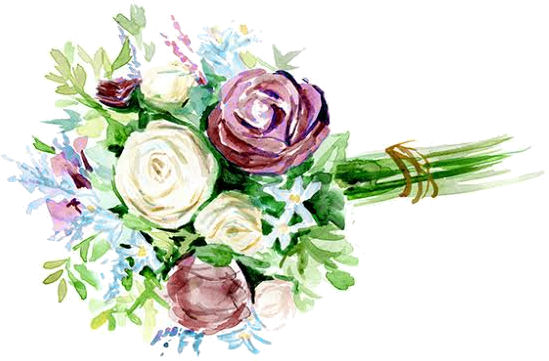
\includegraphics[width=0.45\textwidth]{graphics/flower.jpg}
\end{center}

        \chapter{A Brief History of Information}

%\textit{``Anything worth knowing is worth writing down"}
%bullseyed723 (reddit.com 2016)

\begin{flushright}
    \textit{``Who among you can laugh and be elevated at the same time?''}
    \\ --- Friedrich Nietzsche
\end{flushright}

The second half of the second decade of the third millennium is in the midst of the digital information age and has been for my whole life. The entire collective wisdom of humanity is readily available to everyone through the information superhighway. Notable exceptions of this triumph of humanity are given to the Amish, members of the Gloriavale commune, high-risk offenders, North Koreans, and the uncontacted tribes of the Andaman Islands. It does seem politically incorrect to equate religious fundamentalists with criminals, a totalitarian kleptocracy, and pre-agricultural civilisation... but it is factually correct. I sincerely believe that the primary directive of information retrieval is to facilitate access to \textit{all} information for every living person on earth... even if it does breach The Prime Directive.

The technology used to represent information has advanced substantially across the millennia of human history, from pictograms of aurochs scrawled onto the surface of palaeolithic cave walls (Figure \ref{fig:cave}) to a digital motion-picture (Figure \ref{fig:picasso}) beamed at the speed of light from a solid-state drive in Google's Datacenter through an optical fibre submarine cable crossing the Pacific Ocean, all the way from the west coast of the North American continent to New Zealand, down the South Island's backbone, through a complex network of exchanges, routers, and switches, entering my computer's CPU at the speed of light, causing trillions of transistors to switch billions of times every second to magically transform this cross-continental signal into a video of Picasso painting a Bull, or otters holding hands, or a panda sneezing.

We are truly Gods, beyond the imaginings of our past selves.

\newpage

\begin{figure}[!tbp]
  \begin{subfigure}[b]{0.49\textwidth}
    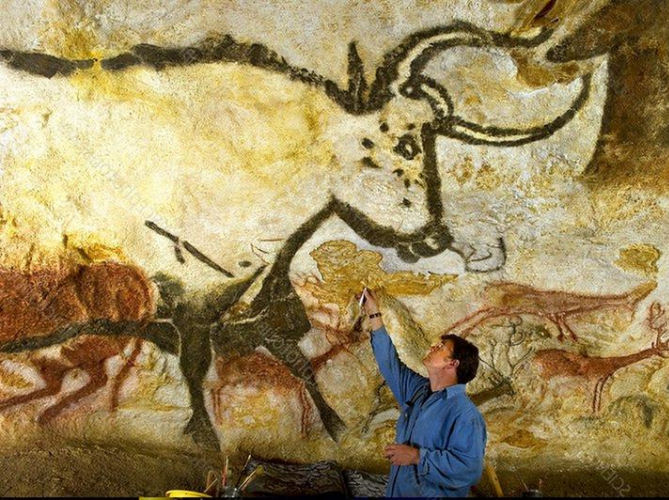
\includegraphics[width=\textwidth]{graphics/bull_cave.jpg}
    \caption{Cave Painting.}
    \label{fig:cave}
  \end{subfigure}
  \hfill
  \begin{subfigure}[b]{0.49\textwidth}
    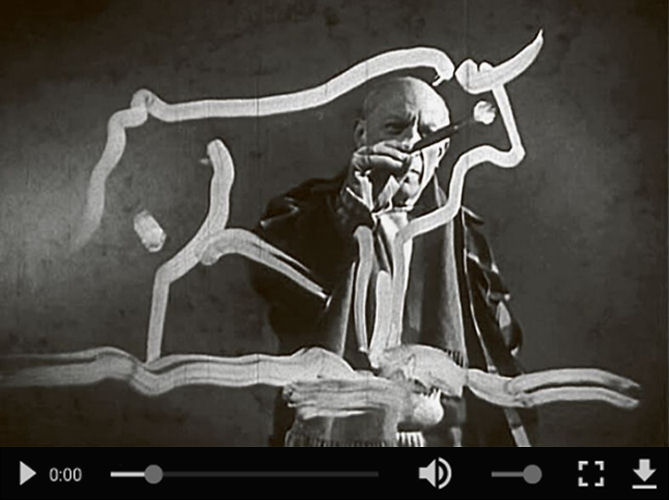
\includegraphics[width=\textwidth]{graphics/bull_picasso.jpg}
    \caption{YouTube Video.}
    \label{fig:picasso}
  \end{subfigure}
  \caption{Information doesn't change, but the format clearly does.
  \\(a) Restoring `Great Hall of the Bulls', painted by humans 17,000 years ago.
  \\(b) Pablo, in the documentary `Visite à Picasso', painting a bull 71 years ago.}% \url{https://youtu.be/W3pfNT6qJUk.}}
  \label{fig:bull}
\end{figure}

\section{The Birth of Books}

A picture may be worth a thousand words, but language is our primary format for information. Archaeology tells us, it was during the Bronze Age when we first attempted to ensconce wisdom from the storytelling tradition into a permanent written record. Information on parchment and papyrus survived for a thousand years or more, far beyond the 34-year life expectancy of palaeolithic humans\footnote{\url{https://doi.org/10.1002}}. Writing as technology was cheaper, easier, more portable, and more space economical than stone carvings. These extant documents include: \textit{The Epic of Gilgamesh, Rig Veda, I-Ching, Brahmana, The Torah, Homer's Odyssey, Bhagavad Gita} and \textit{Aesop's fables}. These codified oral accounts are famously poetic, as they were designed to be memorized. The rhythm and rhyme help preserve plotline for a much longer time. 

These documents were written during a time when our primitive understanding of causality led us to believe that a certain dance would cause rain to fall, stabbing a doll that resembled our enemy would inflict actual pain, and uttering a curse would rouse the wrath of God(s). This faulty logic is what we would now call ``magical thinking''. These thoughts reinforced by correlated events. Rainfall is inevitable regardless of any prior dancing, but if you always perform a special dance during a drought, then the eventual post-drought rain will always come to pass after your dance.

The smug atheist of today considers these significant documents as mere apocryphal stories, fantastical fairy-tales, theological, and mythical in nature... which is not untrue, but it detracts from the facts... these are our early attempts at understanding our world. These are sincere attempts at academic scholarship that we now call: \textit{History, Astronomy, Meteorology, Mathematics, Natural Science, Medicine, Cosmology, Psychiatry, Ethics, and Metaphysics}. Many ancient observations recorded as facts remain facts to this day: trees grow tall, birds fly higher, and love is all-powerful. However, these documents also contain the pseudo-scientific-mumbo-jumbo that we now call: \textit{Numerology, Naturopathy, Acupuncture, Karma, Reincarnation, Spiritual Ascension, Witchcraft, Voodoo, Baptism, Prayer} and other occult practices. Many are provably unharmful but also provably ineffectual, so they are often practised under the divine blessings of \textit{Placeboeffectus}, the trickster god of quackery and fraud. 

Trying to extract moral wisdom or even useful information from these ancient documents is difficult, as they were written before the pursuit of knowledge had matured into a rigorously reliable artform. Over the past couple thousand years, we have developed: Skepticism, Empiricism, Rationalism, Verificationism, Disinterestedness, and Falsifiability, crucial skills needed to sculpt pristine sculptures of understanding from the messy muck of reality.

\section{The Greeks Wrote Books}

Today, people take great pride in the number of books they've read, which is a recent trend as for the majority of human history, nobody was expected to be widely read. Even academic scholars read a measly pittance of books, but they read them well, and they read them often. This is clear when considering religious cultures: the Muslim's Qu'ran, the Jew's Torah, the Hindu's Bhagavad Gita... Even the good citizens of Ancient Greece were expected to know Homer's Odyssey and The Iliad. These weren't just epic tales; they were comprehensive compendiums of wisdom teaching courage, kindness, honesty, and justice. 

Greek wisdom survives through these Ancient Greek Myths, different from Modern Greek Myths, like the long term sustainability of national debt. The secular wisdom and philosophy of the Ancient Greeks form the structural foundation of western civilization. The most famed philosophers are the big three. \#1: Socrates, who gave us the examined life, the interrogative method, and he also taught \#2: Plato, who formalised justice and ideas, and he taught \#3: Aristotle, the first aristocrat\footnote{Strictly in a linguistically non-anachronistic sense.} and polymath, the most influential of the three as he wrote the most prolifically. He is credited with dividing worldly knowledge into the disciplines that persist to this day: \textit{Physics, Biology, Mathematics, Ethics, Politics, Art, Poetics...} Although not everything Aristotle wrote is revered; he propagated the geocentric solar system, that slavery is necessary, that the speed of falling objects is proportional to mass, and that women are the inferior sex: as they are passive, more deceptive, complain more, and have fewer teeth!\footnote{I too would complain more if Aristotle accused me of inferiority after undercounting my teeth.}

From this era survives the work of countless great thinkers: Pythagoras, Zeno, Euclid, Archimedes, Eratosthenes, and my two favourites Epicurus and Diogenes of Sinope. Along with the invention of writing, the other major catalyst for the information boom of Antiquity was the invention of currency. Money facilitated individuals to accrue wealth, allowing them to spend less time toiling and more time writing. Currency wasn't an isolated incident; it spread fast, giving rise to cross-continental merchant trade. The Silk Road united the span of Eurasia; from the West to the East, there were massive escalations in book learning. In the East, this period of history is known as the \textit{Hundred Schools of Thought}, as there were so many thoughts being taught. The most influential thinkers were: Confucius, founder of Confuciusm; Buddha, founder of Buddhism; Sun-Tzu, author of The Art of War; Laozi, author of the Tao-Te-Ching; and the apocryphal man Zarathustra, who \textit{spake thusly}. The thinkers in Persia, India, and China existed simultaneously but largely independently of the Ancient Greeks. While fine silks, wealth, and disease managed to traverse the chain of merchants across the breadth of Eurasia, scholarly information didn't, largely because of the cascade of language barriers but also because commercialising ideas directly wasn't feasible. Thankfully patent law fixed this latter problem until patent trolls ruined it.

\section{The Romans Burned Books}

Greek thought began to spread across the Mediterranean after Aristotle's student, Alexander the Soon-to-be-Great, decided that Greece was a bit too small and not enough people spoke Greek, so he began a campaign of murder until everyone else agreed. Following Alexander's example, everyone else really wanted to have a go at global domination, and for a few centuries, the Mediterranean was consumed with murderous warfare. During this period, vast swathes of literature were lost, science, philosophy, poetry, incidentally destroyed as military generals burned cities in conquest. 

The Platonic Academy was destroyed by the Roman dictator Sulla during the Siege of Athens in 86 BC, 38 years later in 48 BC (this was back when we counted backwards) the Great Library of Alexandria was burned, likely by the Roman dictator Caesar during a military invasion. The Great Library of Alexandria was one of Antiquity's most significant research institutes; it held approximately 100,000 books and scrolls. All of them were destroyed during a military invasion, a fitting end to a library indirectly named after Alexander the Great, the man famed for military invasion.

The Roman Republic, triumphant in warfare later succeeded by the Roman Empire, held sovereignty over the West. After they decimated most of Greek culture, the Romans then appropriated what was left: Zeus became Jupiter, Democracy became Imperialism, Shipbuilding became Road building, slavery remained slavery, and wine remained wine.

\section{The Christians Burned Books}

Around this time, some lad called Jesus started preaching love, forgiveness, and magic tricks. He said killing wasn't groovy, so they killed the proselytising raconteur and occult magician, which was totally not groovy. For a couple of centuries, Christianity was outlawed. If alcohol prohibition has taught us anything, it's that outlawed activities are totally groovy and that people will contravene the law by using their bathtubs for clandestine moonshine and baptism. In 313 CE, Emperor Constantine declared Christianity legal. In 380 CE, Emperor Theodosius declared all other religions illegal. By 400 CE, the Roman Empire was in rapid decline, and the rise of Christian dominance was imminent.

Unfortunately, the early Christians were responsible for more destruction than the Roman's were. They deemed most scholarship heretical and morally corrupt, as little of it credited God directly. They purposefully burned books, not as an unfortunate byproduct of war, but with malevolent intent, they defaced books and paintings, smashed statues and temples of education, in a repugnant display of viciously violent fanaticism. From the ashes of the Greco-Roman world arose churches; Philosophy and science were replaced with scripture and reverential poetry. Worse still, under the oppression of Christian orthodoxy, fewer books were published, progress was stifled, education of the masses waned in favour of blind, ignorant dogma.

What the early Christians started, the Goths, Huns and Vandals continued. Centuries of progress was irretrievably lost, with religious zealots largely to blame. Some estimate that as much as 90 percent of the literature of antiquity was lost \cite{rohmann2016christianity}. Most of our knowledge of Antiquity survives through partial fragments, brief summaries, and later commentaries. Less than a quarter of Aristotle's works survive\footnote{\url{http://www.rmki.kfki.hu/~lukacs/ARISTO3.htm}}. Most other scholars weren't as lucky; the Epicurean philosophy of happiness persisted as a popular lifestyle for centuries until Christianity deemed it heretical. And of Epicurus's 300 works, almost nothing survived, and it's still more than most \cite{kenny2010new}. 

How crippled would our future society be if the works of Shakespeare, Newton, Einstein and Freud were lost today? This was a dark end; religious extremists, power hunger warlords, and sadistic barbarians irretrievably destroyed almost every god damned thing.

\section{The Muslims Saved Books}

The 1,000 year period between the fall of Rome, and the rise of the Renaissance, between the 5th century CE and 15th century CE, was a dark time. Under feudalism, cultural and economic deterioration plagued us, as did actual plagues. We call this era the Dark Ages or Middle Ages... however, the Middle East calls this era The Islamic Golden Age. My Anglo-Christian education failed to inform me of this information boom. 

At the heart of this era was the House of Wisdom in Baghdad, a library that homed academics who rivalled the Ancient Greeks and preempted much of Renaissance philosophy. After the Prophet Muhammad wrote the Qur'an, the Lexicographer Al-Khal\macron{i}l wrote the first dictionary. While one of these books was taken as gospel, the other was an actual significant human achievement. Mathematician Al-Khwarizmī ---Father of Algebra--- revolutionised Algebra, Arithmetic and Trigonometry with the bleeding edge technology of Hindu-Arabic numerals. Polymath Avicenna wrote \textit{``the''} textbook on medicine which prevailed until the 19th century CE. His \textit{``flying man"} thought experiment explicated the mind-body duality that the Christian philosopher Descartes repeated 600 years later with \textit{``Cogito Ergo Sum"}. Why does Descartes get the credit? Philosophy is Groundhog Day, and language barriers between cultures impinge progress. Most importantly, the Islamic scholars of this era recovered some books from Ancient Greece... they translated these works, wrote commentaries, built upon them, adopted their ideas, which unfortunately included much of Aristotle's misogynistic opinions, which were used to defend their own misogynistic practices: like a pre-millennium Christian using the Bible to defer the blame of their own rampant homophobia. However, the foundation of modern scholarship rests on Aristotle's shoulders, and if they had been lost, our progress could have been set back centuries, so we thank our Islamic brothers. 

Unfortunately, history repeats itself. In 1258 CE Baghdad was sieged, The House of Wisdom and its contents were destroyed, the Mongols were to blame, lead by the notorious Genghis...

\begin{center}
\textit{``KHAAAN!!!!''}\\ --- Admiral James T. Kirk
\end{center}

\section{The Europeans Refined Books}

Thankfully, not all was lost. Another era of information began when Catholic scholars rediscovered Aristotle (from Islamic commentary) around 1200 CE, 15 centuries after Aristotle's death. Fibonacci reintroduced and popularised the Arabic-Hindu number system; Thomas Aquinas gave us Scholasticism; William of Ockham gave us Ockham's razor, and Duns Scotus gave use the pejorative \textit{``Dunce''}. Unfortunately, this rising force of scholastic scholarship ended abruptly in 1346 CE with the Black Death, the largest population decimation in human history, taking a mere four years to kill half of all Europeans, faster even than COVID eradicated Trump supporters.

Across the globe, there have been many information booms, separated by information winters, caused primarily by warfare, disease, and the bigotry of the religious. It was not until the mechanical printing press was developed in the mid 15th century (1440 CE) that an information boom could permanently take hold, as books could be produced at a rate significantly faster than they could be destroyed.

% The 16th century saw the Renaissance (1494 – 1550) 
% The 16th-17th century saw the Scientific Revolution (1543 – 1687)
% The 18th century saw the Age of Enlightenment (1715 – 1789)  
% The 18th-19th century saw the Industrial revolution (1760 – 1840)

% At the tail end of the industrial revolution started the science and inventions 

% 1833 Science as a profession, "scientist" meaning Knowlegde Artist is invented
% 1959 Darwin's natural selection
% 1861 Maxwell formulates the four Maxwell equations
% 1873 Maxwell published treatise of Electromagnetism

% 1856 Louis Pasteur discovers Pasteurisation
% 1875 Alexander Graham Bell's telephone
% 1879 Thomas Edison's practical incandescent light bulb.
% 1879 Louis Pasteur's laboratory developed vaccine.
% 1885 Louis Pasteur's developed rabies vaccination.
% 1888 drinking straws
% 1890 cardboard box
% 1891 electric kettle
% 1901 vacuum cleaner
% 1903 the teddy bear

The rest of the Scientific Revolution is well known here in the west; we tend to wear our Anglocentric knowledge on our smug sleeves, we keep it right next to our ignorance of other cultures. Francis Bacon gave us The Scientific Method. Galileo fought religious opposition for heliocentrism after Copernicus failed to. Newton, Descartes, Kepler, Leibniz, Spinoza, Pascal, Shakespeare, Locke... all thinkers in the same generation that were not lost, most notably Gutenberg himself, who invented the machine that literally immortalized his name. Followed closely by Voltaire, Euler, Hume, Kant, Rousseau, Watt, Gauss, Darwin, Schopenhauer, Hegel, Schelling, Kierkegaard, Spencer, Freud, Hilbert, Twain, Nietzsche, Planck, Curie, Jung, Einstein, Schrodinger, Wittgenstein, Heidegger, Koestler, G{\"o}del, Turing, Grice, Camus, Feynman, von Neuman, Tesla, Austin, Lacan, Popper, Foucault, Derrida, Sagan... a never ending list, but dominated largely by German men (i.e. citizens of the Holy Roman Empire 2.0).

%Industrial revolution 

%16th Century saw the rise of mass production of books, after the advent of the printing press in the

%12th Century saw the rise of manuscript production

%previous to that was the codex manuscript, which were hand written by authors, and hand written by scribes.

%Wars are driven by economic and political reasons, a greedy desperation for resources, which is unsurprising in a society largely dependent on resources.

This simplified narrative above, the history of information, is pieced together from extant documents. It's incomplete because it leaves out precisely what has not survived, including even what we are unaware of what has not survived. If you doubt any part of this historical timeline you can check Wikipedia as a source of truth, I know it's all on there because I put it there myself. 

I would argue that the greater loss of war is not human life but rather the irreparable loss of information itself. The life of any individual is highly overrated. Death cannot be prevented, only delayed. However, we can prevent the death of information. Information can be immortal, and helping information achieve immortality for our future generations could be humanity's greatest achievement. 

%Historical humanity goes through cycles of information revolution, the rise of scholarship followed by irreversible destruction. The extents of knowledge 



%The myth of Jesus has value, as the myth is immortal, it outlived the man himself.

%The first historical account I've ever seen that doesn't use glorify military commanders, and political leaders... the kinds of people who not only think they can change the world, but also openly claimed to want to change the world... which is just claiming to look marvelous in statue form\footnote{Why is Alexander the Great considered a brilliant military commander, and it's only Hitler and Stalin we call evil. Alexander the Great? more like Alexander the Sycophantic Cunt... war mongering, blood lusting, missionary of death. I wish he was brutally tortured and mutilated as a child, in-order to simultaneously in-act retroactive justice and prevent his serial-killing-spree. And even worse, I wish him forgotten, it's too late, his name is immortal.}.

\section{The Obsolescence of Books}
This brings us to the latest information era, the era of digital information, which started around the birth of the world wide web, a few years before my own birth. We now have an interconnected network of digital Information systems which have heavily changed almost every aspect of our lives, in both trivial and significant ways. It has affected commerce, politics, education, mass surveillance, and most notably in the acquisition of pornography. It's also responsible for an abundance of misinformation and disinformation, like political propaganda, vaccine scepticism, and the Berenstein conspiracy. Such extravagant information replication and proliferation would not be possible with the antiquated paper system of antiquity or word of mouth before that, which is fantastic! As I sincerely believe in unrestricted freedom of information. I cannot fathom a good reason why any knowledge should be forbidden or censored, for when it is, there immediately becomes a sectarian divide between those who know and those who do not, an imbalance that can be used to exploit and manipulate. Even if dissenting ideas are seen as vulgar, objectionable, or spark controversy, they should still be openly shared because there cannot be progress without direct confrontation of controversy. If everyone agrees with the status quo, the status quo will persist long after its expiry date.

\begin{center}
\textit{``I may not agree with you, \\but I will defend to the death your right to make an ass of yourself.''} \\ --- Oscar Wilde
\end{center}

The impressive immediacy of information transmission the internet allows should only increase the rate of progress. However, it is not within the remit of information retrieval research to fully explicate the ethics of digital information. I will leave the proof as an exercise for the reader. My chosen role in society is to improve the platform that distributes information. It is, however, an immutable fact that there is an abundance of knowledge, more than ever in human history, directly at our fingertips. Information Retrieval directly mediates our access to almost all of this information, from the carefully constructed digital libraries of academia, arts and science, to the vast open plains of the world-wide-web, and the underbelly of the darknet (e.g.\ page three of Google). But despite the technological prowess modern internet search engines claim to have, I am still unable to find a serious meaning in the TV series finale of Lost or find a good reason as to why banks are unable to transfer digital currency between databases on a Sunday. There is obviously much progress to be made... the truth is out there!

\begin{center}
    \textit{``Scientia potentia est"} (knowledge is power) 
    \\ --- Francis Bacon
\end{center}

It's widely believed that having knowledge gives you power, which it does, but more than that, knowledge itself \textit{is} power, and humanity is directly subservient to it. We are dedicated to the pursuit of knowledge, and our livelihood depends on knowledge, but it does not depend on us. The essentialist's knowledge exists independently from us; only our own awareness of knowledge depends on our own existence. We willingly search it out, increasing our awareness of it, stacking it up into teetering towers of unread books, filling halls of libraries, gathering dust to symbolise our collective knowledge despite individual ignorance.

What's the difference between knowledge and information? Some say \cite{lucky1989silicon} that there is a hierarchical relationship between wisdom, knowledge, information and data, which is thus:

\begin{center}

Data $\Longleftrightarrow$ Information $\Longleftrightarrow$ Knowledge $\Longleftrightarrow$ Wisdom

\end{center}

There is heaps of data on the net, and provided our perception of time appears to be unidirectional, the amount of data won't reduce (Assuming Scientologists don't burn the Internet). We have managed to amass thousands of years of culture, art, science, technological development and photographs of spiralized courgettes served on toasted pumpernickel at upmarket high street cafes tagged unironically as \textit{\#bourgeoisie} on Instagram. And many of us humans have an urge to retain all of this \textit{``stuff''} for the future benefit of future peoples, for the prosperity of posterity, for nostalgia, and oftentimes... just `coz.

%%%%%%%%%%%%%%%% DATA
\textbf{Data} can be recorded from almost any source. We can even algorithmically generate any arbitrary piece of data. All we need is a surplus of immortal monkeys and unbreakable typewriters to generate anything, the majority of which would be worthless noise. This kind of data is noise; it has no meaning or practical usefulness. However, the information content could be quite high, as uniform-random data has high entropy due to its lack of predictability.

%%%%%%%%%%%%%%%% INFORMATION
\textbf{Information} is data with a provided context; it has some meaning and practical usefulness. We measure information content by its predictability, not by its perceived importance or usefulness. This leads us to the counter-intuitive notion that uniform-random noise contains more information than deliberately structured information. The imposed structure on data provides predictability through redundancies (assuming uncompressed data), e.g.\ for a document written in the English language (part of the context), a \textit{`q'} is very likely to be followed by a \textit{`u'}, even if it is written on a QWERTY keyboard by a Qantas pilot flying to Qatar. The difference between the white noise received on a near-obsolete FM radio and a .mp3 of \textit{``A Candle in the Wind"}; the difference between the echo of the Big Bang's background radiation received through a UHF antenna and a .mov of a cat playing the piano.

%%%%%%%%%%%%%%%% KNOWLEDGE
\textbf{Knowledge} is a wider concept than information; it takes into account the full breadth of the information's context. It describes the connections between pieces of information because facts don't exist independently floating in a void but rather within an interconnected network. A collection of related pieces of information is called a knowledge base or an ontology—an intricately structured model categorising things and their associated relations. A popular model for a digital knowledge base is the Resource Description Framework, representing associations as edges within a directed multi-graph. The great thing about these kinds of knowledge bases is that you can deduce new information by following a chain of inferences, which is far more difficult to do with Relational Databases or Associative Key-Value-Pair Maps.

%You will have already used one of these systems, Google's Knowledge Graph, which is invoked during every web search, and the results are shown in the infobox on the right. 

I assume that all knowledge is perilously close to assumption. Any inference exists on a spectrum between a justified deduction from all the readily available evidence and a bigoted generalization. This is because any knowledge base (digital or mental) is incomplete and full of inaccuracies. Any good knowledge base is not temporally static. It acquires new information and corrects itself over time. Knowledge is rarely consistent. There are frequent exceptions, caveats and contradictions, making it impossible to be certain about almost anything. However, biological minds can still make material inferences and predictions about our reality through an intuitive approach, an enigmatic fuzzy-logic\footnote{Some might say faulty cognitive heuristics.}, rather than a strictly rational system. Our minds have the ability to extract the information from our experiences into ordered schemata and patterns of association, generalisations from which we can intuitively infer. This is why when I was four years old, I told Mum, \textit{``I don't want long hair because I don't want to be a girl.''}. This doesn't mean the pursuit of truth is futile, but it is important to maintain the clarity of the epistemological hierarchy at all times.

%human communicaiton works on assumption and inference.
%indirect speech (implicature, entailment, likelihood disambiguation, presupposition, shared mutual knowledge...)
%Conversation is a cooperative act
%both participants excert cognitive 

%%%%%%%%%%%%%%%% WISDOM
\textbf{Wisdom} is based on the practical application of knowledge and entails either an individual or collective belief in its perceived validity. I can say \textit{``The chicken came before the egg"}, which is definitely a piece of knowledge\footnote{Especially if one trusts Genesis 1:20-22}, but whether it is universally accepted as truth is contentious, and whether it is useful is unclear. 

Here's a more serious example, proverbial wisdom I hear often:

\begin{center}
\textit{``Reliance on digital media is corrupting the youth of today."}
\\ --- Conventional ``boomer'' Wisdom
\end{center}

This is definitely data; there's an informational context; it is relevant and strongly associated with many aspects of my (and your) contemporary lifestyle. But is it wisdom? Is it wise to live our lives by it? Only time and God can tell. And since I can hear neither God nor time, let's contrive a prophecy!

We know that historically the introduction of other forms of media caused widespread scepticism and, in many cases, mass panic. When television became popular, there was fear that we'd never talk to each other; we'd stare at the fluorescent screens like zombies; there would no longer be a conversation over the dinner table ever again. Telephones were also thought to end the family's chat-chat as the phone's ring would draw attention away, attention spans would be disrupted because you'd be constantly interrupted. Going back even further, to when writing became hip in Ancient Greece, literacy was considered by many to be degenerate and decadent, and your memory was expected to deteriorate due to neglect. There was a genuine fear that people would not cultivate their memory since one could write everything down and lazily refer to it later. Now since you are likely reading this sentence in print, I shall refrain from convincing you of the value of literacy; you're already part of the system, it's too late for you.

I wouldn't claim that digital media is all pristine peaches and refined roses, but the benefits surely outweigh any detriments by orders of magnitude. So it stands to reason that fearing the rise of digital media is merely unfounded speculation, which is in line with the human tradition of delusional mass panic. The uncertainty of the future is certainly frightening; we have no assurance that anything will be O.K.\footnote{O.K. a joke from the 1840s, an ironic misspelling of \textit{All Correct} (\textit{Oll Korrect}).}. The existential malaise is omnipresent. It's natural to justify this fear by contriving an argument against the unknowable effects of digital media or some other new-fangled technology. Because there is no genuine prophetical oracle, there cannot exist any certain affirmations that would dissuade the conservative pessimists that plague progress. But with patience, time will prove wrong the negative Nancy's and doubting Thomas's who fight progress, as it has done, again and again and again. I, for one, do not mourn the loss of the hunter-gatherer jobs that were lost during the rise of agriculture.

%The future is by virtue of itself uncertain, the past however is 
%fondly nostalgical
%it's certainty is reassuring

%It takes courage to venture into the future, in fact you can't be courageous without fear.

%technological obsolescence
%I for one do not mourn the loss of the hunter-gatherer jobs that were lost during the rise of agriculture
%I refuse to light my home with electric light bulbs, support the candle industry! 
%I refuse to use photocopiers, support the scribe industry!

%The long-term goal of any society should be complete unemployment

%I do not understand the obstinate refusal to stand on the shoulders of giants

That was supposed to be wisdom, of a polemic flavour, centrally about the value of digital media and information retrieval. The point is, we should rejoice, as it appears there are more signs that our society is heading towards a Star Trek utopia, not a Mad Max dystopia. So what can we do to improve our communication with these digital information systems?
    
    \part{Literature Review}
        \chapter{Search Engines} \label{chap:searchengines}

\begin{flushright}
    \textit{``A serious and good philosophical work could be written consisting entirely of jokes.''}
    \\ --- Ludwig Wittgenstein
\end{flushright}

%%%%%%%%%%%%%%%%% Information Retrieval
Information Retrieval (IR) is the data-driven field of Computer Science dedicated to creating systems that can retrieve specific piece(s) of information on request from within unfathomably massive bodies of information. It is integral to: genome mapping, spam filtering, plagiarism checking, recommendation systems (YouTube, Netflix, ...), and unsurprisingly: search engines, which are the primary focus of this thesis. Search engines are the IR systems that allow people to retrieve information from medical databases, academic libraries, and the World-Wide-Web. Commercial Search Engines include: PubMed, Google Scholar, and most notably Google Web Search\footnote{At the outset of my Master's research, I hoped Google would eventually hire me, but now I would rather keep my soul uncorrupted.}.

%%%%%%%%%%%%%%%%% Information Need
\section{Information Need}
When a user wishes to know something, we say they have an \textit{information need}; they desire to obtain some specific piece of information. A system created to satisfy an information need is called an Information Retrieval Engine or a Search Engine. What makes a good Search Engine? A quality search engine should be intuitive to use, quick to retrieve, also accurate and comprehensive in what it retrieves. For example, a doctor may have an urgent need to know the treatment for \textit{Chronic Decollatio}\footnote{What are the long term side-effects of decapitation?}. From a database of medical knowledge, a competent search engine would provide all possible treatment options. no more; no less. Retrieving \textit{all} the relevant information and \textit{only} the relevant information promptly and in a user-friendly way is a monumental task, considering the potentially tremendous amount of data to be sifted through.
%Factor (1) is preferential, (2) is relativistic, (3) and (4) however are crucial, and are usually called \textit{recall} and \textit{precision}.

For Web Search, a user's intent is commonly classified into these three broad categories: Informational, Transactional, and Navigational \cite{broder2002taxonomy}. Navigational intent is when a user does not know, forgot, or cannot be bothered typing a web URL. Transactional intent indicates the user is looking for a web service or resource, e.g. ecommerce purchase. Finally, Informational intent is when a user wishes to learn something. In web search, around 50\% \cite{broder2002taxonomy} and 80\% \cite{jansen2008determining} of all web searches have informational intent; they are also the hardest to monetise\footnote{But not impossible, e.g.\ hiding academic papers behind a paywall.}.

% This thesis will disregard both transactional and navigational as data-sets for these tasks are kept secret by commercial entities.

%%%%%%%%%%%%%%%%% Search Queries
\section{Search Query}
Before the search engine can fulfil any informational requirements, the user must communicate their desire(s) through a request known as a \textit{search query}. The query is a representation of their information need, which is understandable by the search engine. Queries are often expected to be plain text but could be any form of media (e.g.\ image, sound clip). Text queries can be processed by one of three main retrieval systems: knowledge, data, and text \cite{lewis1996natural}.

%%%%%%%%%%%%%% KNOWLEDGE RETRIEVAL
\textbf{Knowledge retrieval} is the most sophisticated of the three and requires complex linguistic comprehension of the query. From answering simple trivia questions to more abstract problem solving, knowledge retrieval aims to emulate the cognition of a human mind if it were infallible and more omniscient. Deep learning's advances in Natural Language Understanding (NLU) approaches (e.g.\ OpenAI's GPT or BERT) already outperform non-experts \cite{wang2019superglue}. After the query has been \textit{``understood''}, the system then traverses a highly structured and content-rich ontology (knowledge graph) to \textit{generate} an answer specific to the user's request. Commercial examples include Google's Knowledge Graph \cite{singhal2012introducing}, and WolframAlpha, the freely available Computational Knowledge Engine \cite{wolfram2012wolframalpha}.

% \footnote{These systems struggle at identifying nonsense, for example, I asked WolframAlpha ``how many years between 11 April 1994 and the height of Mount Everest?'', and it replied ``16.75 years"}

%%%%%%%%%%%%%% DATA RETRIEVAL
\textbf{Data retrieval} also makes use of structured information: spreadsheets, relational databases, or even ontologies. The main distinction from knowledge retrieval is that the queries require a structure that is not a natural language, e.g. Structured Query Language (SQL) for Relational Databases. These formal query languages are technical in nature and are not intuitive to use. Not only must the query language's grammar be learned, but specifics of the data structure must also be known. Therefore, the barrier to entry for the average user is reasonably high. Another difference is that the system does not generate information per se; it can only retrieve a subset of its containing data. The caveat is some fancier query languages allow for explicit processing directives, which perform minimal computations on the retrieved data.

% . An ideal search engine would be able to understand unstructured and arbitrary queries, i.e.\ written in a human language.

%%%%%%%%%%%%%% TEXT RETRIEVAL
\textbf{Text retrieval} is the most common system. It is designed for unstructured, semi-structured, or information that has a structure but is unknown to the retrieval system. This makes it ideal for websites, newspapers, books, and any other text document format. This is why it is often called \textit{Document retrieval}. Although text retrieval usually retrieves entire documents, there is also \textit{Passage Retrieval} which retrieves excerpts from within documents. Text retrieval performs search tasks not through \textit{``understanding''} information but rather through probabilistic assumptions between the user's query and the relevant documents.

\begin{table}
\begin{center}
\begin{tabular}{l|l|l|}
\cline{2-3}
                                          & Query                     & Information                    \\ \hline
\multicolumn{1}{|l|}{Knowledge Retrieval} & Natural Language          & Complex data structure         \\ \hline
\multicolumn{1}{|l|}{Data Retrieval}      & Structured                & Simple data structure          \\ \hline
\multicolumn{1}{|l|}{Text Retrieval}      & Unstructured (ad-hoc)     & Unstructured / Semi-structured \\ \hline
\end{tabular}
\end{center}
\caption{Comparison of retrieval types} \label{tab:retrievaltypes}

\end{table}

Many text retrieval systems support meta directives, much like data retrieval. For example, \textit{Boolean Retrieval} supports boolean operators within the query, e.g.\ the NOT operation excludes query terms. Most commercial systems support various directives to help the IR system, including ``double quotes'' that make terms required and/or define their order.

%%%%%%%%%%%%%% ADHOC QUERIES
The queries in text retrieval are unstructured, much like knowledge retrieval. The query is required only to be a string of word(s); however, there is no expectation the user will adhere to the language's grammar rules or even be comprehensible by conventional standards. This is often called \textit{ad-hoc retrieval}, and a series of keywords is often sufficient to form an ad-hoc search query. Most contemporary internet search engines accept this kind of free-form query construction. A query has a much higher chance of success if it is somewhat well-formed, but a quality search engine can handle typos, misspellings, even incomprehensible gibberish. For example, if one types a query into Netflix by mashing the keyboard in the chaotic, higgledy-piggledy manner of a fat-fingered, drunken animal:

\begin{center}
    % ``''a3857vb349se7itn7o834tcyweufhsldjkghancrauawmefhsceukt''
    ``asdf;ksa;llfsdfsadfasdk;lfjasjfdk;lasfjldfjsafjdsl;fjajfdlksaj''
\end{center}

\noindent
Netflix will suggest children’s TV shows.

% , which is a feature to be applauded. 

% Netflix will also auto complete titles for movies it doesn't have, which is annoying.

\subsection{Unstructured Information}
Internet websites are the most accessible source of unstructured information, but they are not the only type. An information retrieval system can be constructed for any digital information store, so long as the information store can be discretized into a collection of documents. The content of a single document varies depending on the information domain (e.g.\ academic journals, web pages, images, audio files). Herein we will be focusing only on text documents for text retrieval. The grammar in text documents is ignored by default; they are considered a mere sequence of words (\textit{lexical tokens} or \textit{terms}). Documents may also be considered semi-structured, which is when parts of documents (e.g.\ headings, sections, paragraphs) have been tagged (e.g. XML).

The collection of all documents accessible to the IR system is called the \textit{corpus} or \textit{document collection} and is often massive, in the order of multiple gigabytes in size and potentially significantly larger. We will not be discussing the processes involved in acquiring a collection or adding structure to the documents. You may: scan books at your local library, illegally download ebooks from \textit{Library Genesis}\footnote{Libarary Genesis is located at libgen.is should you wish to avoid it.}, or flout the temporal boundaries of reality to recover scrolls from The Great Library of Alexandria\footnote{I'm seeking a research grant for this project.}. We only require that the documents be converted into digital files so that they can be searched.

%%%%%%%%%%%%%% TERM MATCHING
\section{Estimating Relevance}
Documents are considered relevant if they satisfy a user's information need. It is a binary value judged by the user themselves, either explicitly stated in user studies or implicitly assumed from the user's behaviour. A text retrieval system cannot ever know for certain which documents are relevant, there is always an amount of uncertainty. The output of a relevance model\textemdash Retrieval Status Value (RSV)\textemdash is interpreted as an indicator of relevance, or the probability of relevance, as outlined in the Probability Ranking Principle \cite{jones2000probabilistic} (PRP). There are many relevance models which all essentially perform the same task, they compute some statistical similarity between the document vocabulary and the query vocabulary. For example, if the document contains most (or all) of the query's terms, then the document is assumed to be relevant to the information need. 

% You may have already started to doubt the effectiveness of inferring relevance via a vocabulary comparison, however PRP is proven very effective in practice and the blame for any retrieval failure is placed squarely on the users who construct inadequate search queries (we will explore this topic later).

% Term Matching, Vector Space, Language Modelling

% \textbf{Document Clustering}

\subsection{Term Matching Model}
Term matching estimates relevance by directly matching document terms with query terms, i.e.\ the terms that co-occur in both the document and the query. The document which contains the most query terms is considered the most relevant. The document which contains the fewest or no query terms is considered the least relevant. In short relevance of a document is proportional to the frequency of query terms. Query terms are connected with an implicit OR, so it is not required that every query term occurs in the document. 

% Also known as \textit{Boolean model} or \textit{keyword matching}.

Na{\"i}vely searching through each document in the collection and counting the occurrence (frequency) of each query term can be too slow for interactive search, which is why term matching implementations precompute an index from the collection. The index structure most commonly used is the Inverted File which is much like the index at the back of a book, except instead of a minimal set of keywords, every word in the collection vocabulary gets an entry in the alphabetised list. Each entry in the Inverted File has an associated \textit{posting list} which lists every document that the term appears in, along with the term frequency ($\mathit{tf}$). Our example documents will be ``fruits.txt'', ``iPod.doc'', and ``apple-pie.pdf'' with respective document ids: 1, 2, and 3. If the word ``apple'' appears five times in the document ``fruits.txt'', 12 times in the document ``iPod.doc'', and eight times in the document ``apple-pie.pdf'', then the posting list for the entry ``apple'' might look like this:

\begin{center}
    index\big[ ``apple'' \big] $\Rightarrow$ \big[ (1, 5), (2, 12), (3, 8) \big]
\end{center}

Now, if a query includes the term ``apple'', the system need only find the entry for ``apple'', which is quick given that the entries are alphabetised, then provide the user with the three document ids in the postings list. An index may also record the document frequency ($\mathit{df}$), which is the number of documents that contain a particular term. For ``apple'' the $\mathit{df}$ would be 3.

\subsection{Vector Space Model} 
An alternative to term matching as a relevance model is Vector Space. Imagine a multidimensional space, V-dim, where every unique word in the collection vocabulary has its own dimension. Documents and queries can be placed in this space where their coordinates on each axis are equal to the frequency of each word in the document. Relevance is estimated from cosine similarity within the vector space or the Euclidean distance if we normalize for document length. 

% Another vector space approach uses machine learning to find vector representation of words e.g.\ Google's Word2Vec and Facebook's fastText.

% Something about clustering?

% Something about Binary Independence Model

\subsection{Query Likelihood Model}
The third relevance we will look at is based on Language Modeling (LM). The Query Likelihood Model considers sequences of words as conditional probabilities. Language Models have seen huge success in speech recognition, search engine autocomplete, and predictive text on smartphones. 

Let us consider a language model not as a word predictor but rather as a random word generator, and every unique document in our collection has been generated by a unique LM. Each of these LMs can be prompted to generate a string of words that have the same vocabulary distribution as the original document\footnote{I attempted to generate jokes with a Markov chain implementation of an LM with zero success.}. Each word does not have an equal chance of being generated, but rather each word's probability is relative to its occurrence in the original document. For example, the language model for The Holy Bible would generate the word \textit{``miracle''} more frequently than the language model for Darwin's On the Origin of Species (specifically 4x higher, see Table \ref{tab:miracle}). A language model for Islamic religious texts would likely generate the phrase \textit{``Peace be upon him''} immediately after generating the word \textit{``Muhammad''}, as it is the Durood Shareef tradition prolific in Islam. 

The Query Likelihood Model estimates a document's relevance by the likelihood that its language model would generate the user's search query. Most language modelling implementations for IR are unigram models or \textit{Bag-of-words} models, which assumes the word order and grammar aren't important, but the occurrence (or frequency) of each word is important. Unigram models are often sufficient for text retrieval as queries are considered to be ad-hoc. Bi-gram and n-gram models account for word order, but they are much less efficient and suffer from data sparseness, i.e.\ documents and collections too small to calculate comprehensive and accurate models from.

\begin{table}
    \begin{center}
        \begin{tabular}{llll}
        \cline{2-4}
            \multicolumn{1}{l|}{}
            & \multicolumn{1}{l|}{The Holy Bible}
            & \multicolumn{1}{l|}{Origin of Species}
            & \multicolumn{1}{l|}{This Document}
        \\ \hline
            \multicolumn{1}{|l|}{Word count}
            & \multicolumn{1}{l|}{727,969}
            & \multicolumn{1}{l|}{208,415}
            & \multicolumn{1}{l|}{32,382}
        \\ \hline
            \multicolumn{1}{|l|}{\textit{``miracle''} count}
            & \multicolumn{1}{l|}{42}
            & \multicolumn{1}{l|}{3}
            & \multicolumn{1}{l|}{17}
        \\ \hline
            \multicolumn{1}{|l|}{\textit{``the''} count}
            & \multicolumn{1}{l|}{83,702}
            & \multicolumn{1}{l|}{14,581}
            & \multicolumn{1}{l|}{1,782}
        \\ \hline
            \multicolumn{1}{|l|}{\begin{tabular}[c]{@{}l@{}}\textit{``miracle''} proportion\end{tabular}}
            & \multicolumn{1}{l|}{0.0000576}
            & \multicolumn{1}{l|}{0.0000144}
            & \multicolumn{1}{l|}{0.0005475}
        \\ \hline
            \multicolumn{1}{|l|}{\begin{tabular}[c]{@{}l@{}}\textit{``the''} proportion\end{tabular}}
            & \multicolumn{1}{l|}{0.1150}
            & \multicolumn{1}{l|}{0.0699}
            & \multicolumn{1}{l|}{0.0550}
        \\ \hline
        \end{tabular}
    \end{center}
\caption{Word counts of ``miracle'' and ``the'' in \textit{The Holy Bible} (NIV edition), \textit{On the Origin of Species} (6th Edition), and this documents itself.} \label{tab:miracle}
\end{table}

\section{Ranking}
The core of any Search Engine is the ranking function. It is the algorithm that calculates the relevance score for each document, then sorts the documents by descending relevance. The document with the highest relevance score is placed in the top rank; the second most relevant document gets the second rank, etc... A fast and simple ranking function is sorting by term frequency, i.e. the document which contains the most query terms is ranked the highest. However, this simple approach is not the most accurate. Currently, the most accurate way to rank documents is with machine-learned ranking (MLR) or learning to rank methods. The downside to MLR is the comparatively slow speed on massive document collections. For interactive web search, users expect retrieval results in a few milliseconds, and the web contains billions of documents, which is why modern web search performs ranking using both MLR and more simple ranking algorithms \cite{baeza1999modern}. This is known in the literature as a multi-tier ranking pipeline \cite{risvik2003multi}, a cascade of document filters the incrementally reduce the document collection into a more manageable size. The lowest tier performs top-$k$ document retrieval, reducing billions of documents down to a few million (or a few thousand). This smaller subset of the document collection is then re-ranked in the higher tiers with much slower but far more accurate MLR methods. The focus of this thesis is on the lowest tier of the ranking pipeline.

% then a final optional phase involves manipulating the top results depending on how much each document author has \st{bribed} paid the search engine provider.

% Web Search is usually performed on distributed architecture due to the vast nature of the collection
% Fagin's algorithm, Threshold Algorithm (TA), probabilistic TA sorted, Linear Programming adaptation of TA

% Google Web Search uses the proprietary PageRank algorithm, technically nobody outside of Google knows how it works... but in theory, web pages are ranked higher relative to how much you bribe the grubby, money-hungry fuck pigs who run Google.

% One could rank based on the output of your chosen relevance model alone (Vector, Likelihood, or term matching)


\subsection{TF-IDF Ranking}
Na{\"i}ve ranking assumes that all words in a language are of equal importance, which they are not, as some terms are more \textit{discriminating} than others. The most common word in both Darwin's seminal book and The Holy Bible is \textit{``the''}, occurring roughly once every 10-16 words (see Table \ref{tab:miracle}). This probability is similar for many documents written in English. If a query and a document contain the term \textit{``the''}, it does not necessarily indicate relevance to the information need as most documents contain the word \textit{``the''}. We are most interested in terms that uniquely identify, what we might call \textit{discriminating terms} or \textit{content bearing terms}. These words are identified by being uncommon across the collection but overly-prevalent in specific documents. A word like \textit{``miracle''} fits the description and would easily discriminate documents about miracles from documents with no association with miracles\footnote{According to Table \ref{tab:miracle}, the word \textit{``miracle''} is more prevalent in this document than The Bible. Is this document about miracles? The fact I managed to finish this thesis is miraculous.}.

The most common words in a document collection are called \textit{stop words}. They may be explicitly excluded in a relevance model as they are almost always grammar particles (e.g.\ articles, conjunctions, prepositions) and carry little to no information. However, US linguist George Zipf has provided a much better way to handle these common words in what is known as Zipf's law \cite{zipf1949human}, which is analogous to findings by Claude Shannon described independently around the same time \cite{shannon1948mathematical}. It is a linguistic phenomenon that has since been observed in over 50 human languages \cite{yu2018zipf}. Zipf's law was brought in to IR research in 1972 by Karen Sp{\"a}rck Jones \cite{jones1972statistical}, who stated that if we plot the rank of words in decreasing order against their frequency, it matches a discretized power law. There is an exponential relationship between a word's occurrence across a document collection and its ability to discriminate documents.

Sp{\"a}rck Jones suggested that terms could be weighted by the inverse of their collection frequency, as a measure of term specificity, which later became known as \textit{inverse document frequency} or IDF. It is normally calculated as the total number of documents $N$ divided by the number of documents which contain the term ${df_{t}}$. If terms are weighted by their IDF, it will boost the contribution of content bearing terms and diminish the contribution of non-discriminating terms, which has proved to be extraordinarily robust and forms the basis of the many ranking functions in use today: TF*IDF, which sums the product of each query term's frequency ($\mathit{tf}_{td}$) with the IDF.

\begin{equation} \label{tfidf}
    rel(d) = \sum_{t \in Q} \mathit{tf}_{td} \times \frac{N}{df_{t}}
\end{equation}

Improvements on Sp{\"a}rk's IDF include taking the log of the quotient, as the contribution of inverse document scores do not scale linearly but rather sub-linearly. Also, the inclusion of parameters for the estimated number of relevant documents and smoothing corrections \cite{robertson1976relevance, robertson1997relevance}, known in the literature as the Robertson-Sp{\"a}rck Jones (RSJ) weight.

\begin{equation} \label{tfidfrsj}
    rel(d) = \sum_{t \in Q} \mathit{tf}_{td} \times \log_{10}\left(\frac{N - df_{t} + 0.5}{df_{t} + 0.5} + 1\right)
\end{equation}

This allows content bearing terms to have a larger contribution to the relevance estimate, and common words like \textit{``a'', ``the''}, and \textit{``and''} to have negligible contribution.

% The IDF component scales the RSV by taking into account the frequency of a query term across the entire document collection. If a term is contained within the majority of the collection (e.g.\ `the'), it is not considered a discriminating term, so its contribution to the RSV is negligible. But if the term is only contained within few documents, then it is considered highly discriminating, and has a large contribution to the final RSV. 

% hapax legomena
% Google Whack














\subsection{Okapi BM25}
TF*IDF has many variants and influences, including Okapi BM25, one of the most successful retrieval models. Okapi BM25 (BM25) is a probabilistic relevance ranking algorithm devised by Robertson and Walker in 1994 \cite{robertson1995okapi}. Its mathematical foundation is a unigram Language Model based on research by Harter \cite{harter1975probabilistic}, who showed that a document's terms could be modelled as a mixture of two distributions, each with different means. One distribution of terms appears uniformly random across the document collection and provides little value for search, and the other distribution of \textit{specialty} terms which are far more valuable for search. BM25 assumes that all term frequencies conform to a Poisson distribution, a discrete probability distribution where subsequent document terms are modelled as events in time.

%%%%%%%%%%%%%%%%%%%%%% Aboutness
The other key idea of BM25 is the notion of \textit{eliteness}. Every term in the collection vocabulary is thought to represent a concept. Each document can be \textit{about} one or more concepts, where \textit{aboutness} is an unknown feature of documents. If a term appears in a document and the document is \textit{about} the term's concept, then the term is \textit{elite} for that document. For example, both The Holy Bible and Darwin's Origin of Species contain the term \textit{``miracle''}. However, only The Holy Bible is \textit{about} miracles. Darwin's book is not \textit{about} miracles. So the term \textit{``miracle''} is elite in The Holy Bible, and it is not elite in Darwin's book\footnote{This example was chosen intuitively as an illustrative example but is also mathematically sound.}.

BM25 treats documents as a linear combination of two Poisson distributions, one distribution for elite terms, the other distribution for non-elite terms; see Figure\ref{bm25poisson}. Since \textit{aboutness} is unknown to the retrieval system, the eliteness is a hidden variable. It is also a binary variable; either a document is \textit{about} a concept or not, the term belongs to either one of the Poisson distributions. Relevance is estimated from the probability of term eliteness rather than term frequency directly \cite{bookstein1974probabilistic, harter1975probabilistic, robertson1995okapi}.

% 0.0028, k1 = 6.4691
\pgfmathdeclarefunction{poiss}{1}{%
  \pgfmathparse{(#1^x)*exp(-#1)/(x!)}%
  }
\begin{figure}
  \caption{BM25's 2-Poisson term distribution(s)} \label{bm25poisson}
  \begin{tikzpicture}
        \begin{axis}[
            height=5cm,
            width=\columnwidth,
            % axis x line=center,
            axis y line=center,
            axis x line=left,
            xtick={0,2,...,19},
            ytick={0.2, 0.4, 0.6, 0.8},
            domain = 0:10,
            samples = 11,
            xlabel style={align=center},
            % xlabel style={text width=8cm},
            xlabel={$\mathit{tf}_{\!\!td}$ : Frequency of term $t$ in document $d$.},
            % xlabel style={right},
            yticklabel style={
                /pgf/number format/fixed,
                /pgf/number format/precision=3,
                /pgf/number format/fixed zerofill
            },
            scaled y ticks=false,
            ylabel style={above}, %rotate=-90},
            ylabel={$P(\mathit{tf}_d|E)$},
            ymax=1, %0.005,
            xmax=10,
            % x post scale=1.4,
            legend cell align={left}
            ]
            \addplot+[blue, mark=*] {poiss(0.25) + poiss(2.5)};
            % \addplot[blue] {poiss(0.25) + poiss(2.5)};
            \addlegendentry{2-Poisson};
            \addplot+[red, mark=square*] {poiss(0.25)};
            % \addplot[red] {poiss(0.25)};
            \addlegendentry{non-elite terms ($E=0$) }
            \addplot+[violet, mark=triangle*, mark options=solid] {poiss(2.5)};
            % \addplot[green] {poiss(2.5)};
            \addlegendentry{elite terms ($E=1$)};

        \end{axis}
    \end{tikzpicture}
\end{figure}

% • Relevance to a query is related to eliteness rather than directly to term frequency, which is assumed to depend only on eliteness.

% term frequencies depend only on eliteness

% • Hypothesize that occurrences of a term in a document have a random or stochastic element

%%%%%%%%%%%%%%%%%%%%%% Features of BM25

\begin{equation} \label{eq:BM25}
	RSV(d) = \sum_{t \in Q}
	\text{IDF}(t) \times
	\frac{(k_1 + 1) \times \mathit{tf}_{\!\!td}}{k_1 \times \Big((1-b) + b \times \Big(\frac{L_d}{L_{avg}}\Big) \Big) + \mathit{tf}_{\!\!td}} 
\end{equation}

In practice, BM25 can be viewed as an extended TF-IDF model, see Equation~\ref{eq:BM25}. It performs a sum over every term $t$ in the query $Q$, where each summand is a product of an Inverse Documents Frequency (IDF) component and a Term Frequency (TF) component. 
% The original TF-IDF model was based on intuition and experimental research as was BM25, however BM25 has since a strong theoretical foundation \cite{idftheory}.
The IDF component is usually a variant of the RSJ weight, and the TF component is the 2-Poisson representation of the LM. BM25 provides two tunable parameters. The first is $k_1$, which controls the \textit{saturation point}. Saturation is a feature that asymptotically diminishes the contribution of large term frequencies as probabilistic relevance does not scale linearly with an increase in $\mathit{tf}$, but rather sub-linearly. For example, the manual for my car mentions the term \textit{``Tesla''} orders of magnitude more frequently than most online reviews about my car. However, the manual is not orders of magnitude more relevant to the query: \textit{``Tesla model S 100D review''}. The main benefit of the asymptotic limit is to prevent over boosting. If this is not done, we risk one of the query terms dominating the rank and the less frequent \textemdash but equally important\textemdash terms having a relatively inconsequential contribution. 

The shape of the saturation function can be clearly visualized by fixing the parameters and plotting RSV against $\mathit{tf}$, which can be seen in Figure~\ref{tfm}. It is clear that the first few occurrences of term $t$ have the largest effect, after $\mathit{tf}_{\!\!td} > 10$ the RSV begins to plateau. The Figure~\ref{tfm} also compares the BM25 to unmodified TF*IDF, which increases without bound.

%$L_d = L_{avg}$, $k_1 = 0.9$, $b = 0.4$, asymptote at $k_1+1$.
% Parameters fixed for simplicity: $L_d = L_{avg}$, $k_1 = 0.9$, $b = 0.4$.

\begin{figure}[h]
% \baselineskip
% \baselineskip
% \vspace{-1cm}
  
  
  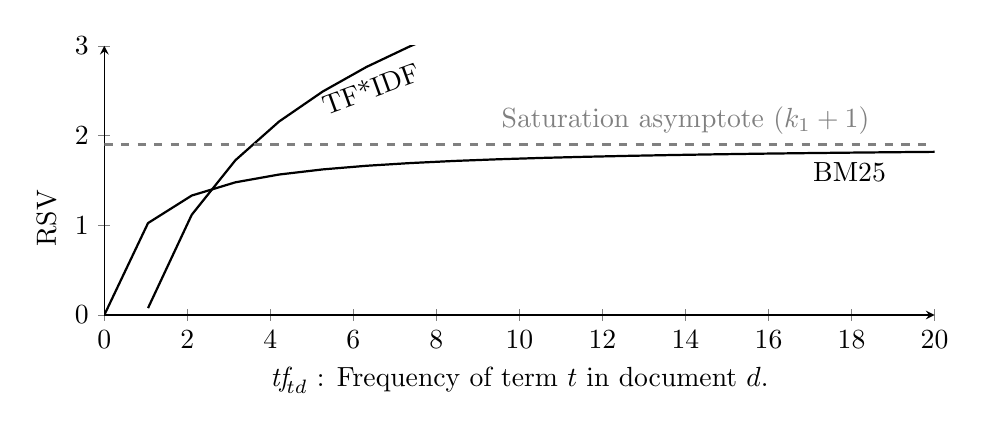
\begin{tikzpicture}
    \begin{axis}[
    	height=5cm,
        width=\columnwidth,
        xmin=0, xmax=20,
        ymin=0, ymax=3,
        % axis x line=center,
        % axis y line=center,
        axis lines = left,
        xlabel style={align=center},
        ylabel style={above left},
        % xlabel style={text width=8cm},
        xlabel={$\mathit{tf}_{\!\!td}$ : Frequency of term $t$ in document $d$.}, 
        ylabel={RSV},
        % title={\Large{BM25 term frequency component}},
        samples=20]
        \addplot[black, thick, domain=0:20, range=0:3] {ln(x) * 1.5} node[below,pos=0.3, rotate=20] {TF*IDF};
        \addplot[gray, thick, dashed, domain=0:20, range=0:2] {1.9} node[above,pos=0.7] {Saturation asymptote ($k_1 + 1$)};
        \addplot[black, thick, domain=0:20, range=0:2] {(x*1.9)/(x+0.9)} node[below,pos=0.9] {BM25};
        
      
    \end{axis}
  \end{tikzpicture}
  \caption{Comparing TF*IDF with BM25 ($L_d = L_{avg}$, $k_1 = 0.9$, $b = 0.4$)} \label{tfm}
\end{figure}


%%%%%%%%%%%%%%%%%%%%%% Document Length

The other parameter $b$, controls document length normalization. Early IR research was intended for small documents, e.g. titles and abstracts, but with the scale of the internet and faster computers, it has become expected to search on book-length documents. BM25 is indifferent toward document length ($L_d$) since it normalizes for average document length ($L_{avg}$). The parameter $b$ adjusts the influence of the normalization for collection-specific tuning ($b=0.75$ by default). 

The effect of different document lengths can be seen in figure \ref{bm25doclen}. The document that is four times the average length takes many more terms to reach saturation, and the shorter document requires fewer terms to reach saturation. This makes intuitive sense since shorter documents contain fewer terms, it should not require as many terms to be confident the document is relevant. Much longer documents like books necessitate a much larger $\mathit{tf}$ to be confident in the relevance. The longer a document is, the more likely it will contain infrequent uses of words that falsely appear to be content-bearing terms but used in non-elite ways, possibly in metaphorical ways, e.g. \textit{``miracles of nature''}.

\begin{figure}
% \baselineskip
% \baselineskip
% \vspace{-1cm}

  
  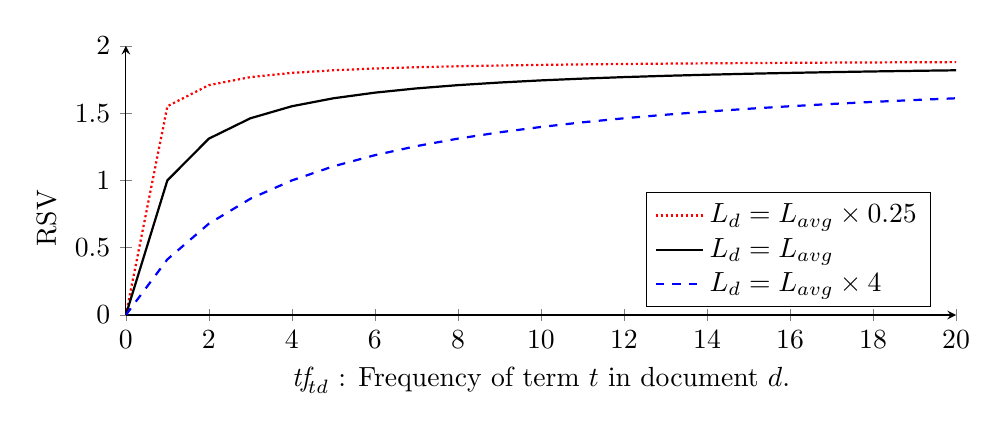
\begin{tikzpicture}
    \begin{axis}[
    	height=5cm,
        width=\columnwidth,
        xmin=0, xmax=20,
        ymin=0, ymax=2,
        % axis x line=center,
        % axis y line=center,
        axis lines = left,
        xlabel style={align=center},
        ylabel style={above left},
        % xlabel style={text width=8cm},
        xlabel={$\mathit{tf}_{\!\!td}$ : Frequency of term $t$ in document $d$.}, 
        ylabel={RSV},
        % title={\Large{BM25 term frequency component}},
        samples=21,
        legend pos=south east,
        legend cell align={left}
        ]
      \addplot[red, thick, densely dotted, domain=0:20, range=0:2] {(x*1.9)/(x + 0.9*(0 + 1*0.25))};
      \addlegendentry{$L_{d} = L_{avg} \times 0.25$}
      \addplot[black, thick, domain=0:20, range=0:2] {(x*1.9)/(x + 0.9*(0 + 1*1))};
      \addlegendentry{$L_{d} = L_{avg}$}
      \addplot[blue, thick, dashed, domain=0:20, range=0:2] {(x*1.9)/(x + 0.9*(0 + 1*4))};
      \addlegendentry{$L_{d} = L_{avg} \times 4$}
    \end{axis}
  \end{tikzpicture}
    \caption{Varying document length ($L_d$) in BM25 ($k_1=0.9$, $b=1.0$) } \label{bm25doclen}
\end{figure}

% Other ranking function may also consider the position of the query terms within the document, in which case the posting lists of the index must record the position(s) of the terms alongside the term frequency.

% Retrieval Status Value (RSV)



% \begin{equation} \label{BM25}
% 	RSV(d) = \sum_{t \in Q}
% 	\log_{10}\left(\frac{N - df_{t} + 0.5}{df_{t} + 0.5} + 1\right)
% 	\times
% 	\frac{
% 	    (k_1 + 1) \times \mathit{tf}_{\!\!td}
% 	}{
% 	    k_1 \times \Big((1-b)+b \times \Big(\frac{L_d}{L_{avg}}\Big) \Big) + \mathit{tf}_{\!\!td}
% 	}
% \end{equation}
% 	\times
% 	\frac{(k_3 + 1) \times qtf_t}{k_3 + qtf_t}

% Original Okapi: k1 = 2, b=0.75

% BM25: k1 = 1.2, b=0.75

BM25 has many features which make it ideal for practical implementations and not just theoretical musings. If $\mathit{tf} = 0$ then the retrieval score will also be zero. The RSV increases monotonically with term frequency, i.e.\ a rise in $\mathit{tf}$ will never reduce the retrieval score. Both vector space and language modelling have influenced BM25 and its extensions. 


\section{Problems With Relevance Models}
%%%%%%%%%%%%%%%%%%%%%%% short queries
One issue with ad-hoc retrieval is that it expects users to write adequate search queries. Unsurprisingly users often fall short of expectations. Firstly, their queries are very short. The majority of all queries contain only one, two, or three terms \cite{gabrilovich2009classifying}. According to Rand Fishkin, 79.18\% of Google's web search queries contain three or fewer terms, and searches performed from mobile phones have even fewer terms on average \cite{enge2012art}. With fewer search terms, the probability of them co-occurring within documents is clearly lower than would be expected of a more comprehensive search query.

But the wider problem is using vocabulary to estimate relevance as it makes two assumptions. The first is that the information content of a document is adequately described by the vocabulary it contains. The second is that the information need of a user is adequately described by the vocabulary the query contains. Individually, these assumptions appear to be entirely reasonable, especially when considering a human reader comprehending the information content. However, there is an unfortunate disparity that arises when both of these assumptions are made. Essentially, the query is written by someone ignorant about the vocabulary used in the document collection. And conversely, the document authors cannot predict what vocabulary might appear in a search query.

An extreme example of this disparity is obvious when considering the foreign language barrier. If a monolingual English speaker searches for marital guidance, they can type no query that will ever retrieve something written in Arabic, no matter how relevant the Arabic document may be. This is a shame, as the Qur'an has many great passages on marriage. That isn't a glib joke. The Qur'an's reformation of marriage was progressive for its time: it forbade incestuous marriage (Qur'an 4:23); forbade forced marriage (Qur'an 2:232); though it also allows men to have up to four wives (Qur'an 4:3), no reasonable person would expect a 1,400-year-old moral codebook to perfectly espouse modern ideals. At least it doesn't promote forced incest, like Christian Royalty in England practised.

%%%%%%%%%%%%% MISCOMMUNICATION.... leads to vocabulary emismatch
%%% different authors, disparity, 

%The user is by definition ignorant, they lack some knowledge, specifically the piece of information they are seeking. The user hopes that there exists (or has existed) a person who is not ignorant and has at some point in the past written the piece of information they need within some document in thecollection. There is no guarantee that thecollection even contains such a document. In the most ideal case the query author (user) and document author are the same person. The worst case is when the user knows nothing about the document author.

%Their ignorance can lead them to construct a query which does not describe their information need in the same words as that the document author does. 

%If a search engine fails to retrieve the desired information the user is expected try again, with the query phrased in a different way, this is known as query reformulation.

%So the user cannot be expected to know very much about the information they desire, for if they knew the information, they would not have to query an search engine for it. 

%This ignorance exists because there is no direct communication between the user and the document author(s). 

%Instead the SE is expected to behave as the conduit between them, interpreting the information need of the query and also the information content of thecollection.

%Human to machine communication

%Interaction between authors and information requesters
%There is no direct, no immediate cooperation
%allude to creative vagueness

%to describe the document collection is usually the same vocabulary used to construct search queries. 

%within term matching systems this problem arises as the \textit{Vocabulary Mismatch Problem}

%SEMANTIC DISAMBIGUATION

%%%%%%%%%%%%%% VOCABULARY MISMATCH
\subsection{Vocabulary Mismatch Problem}
Documents written in the same language, on the same subject, with the same intention and focus, can differ greatly in the vocabulary used, also in the dialect and prose. This is because the document's authors themselves differ greatly. They will certainly have different cultural backgrounds, different social upbringing, different degrees of education, and differing opinions on politics and wider ideologies. Their different experiences colour the language of their writing. One author may write \textit{``Mad Cow Disease''}, another more medically trained author may choose to write \textit{``Bovine spongiform encephalopathy''} or even \textit{``BSE''}. All those phrases refer to the same concept. They mean the same thing, however, the language used to describe them bears little lexical similarities, so relevance models that match terms between the query and the document are unlikely to retrieve all the documents relevant to the user's information need.

The vocabulary mismatch problem is rampant in human-generated text. Human authors frequently use different words to describe the same concept. Even domain experts will use different terms to describe the same concept. Experiments have shown that the likelihood of two such individuals using the same term is less than 20\% \cite{Furnas:1987:VPH:32206.32212}. Research more specific to information retrieval has shown that ``Queries dealing with the same topic are extremely variable'' \cite{buckley1999trec} and that variation heavily affects retrieval effectiveness \cite{bailey2015user}. The UQV100 (Unique Query Variability) is a test collection of 10,835 queries sourced from 263 workers who were asked to write queries for 100 specific information finding tasks. The collection records 5,764 unique queries for those tasks after normalization and spelling correction \cite{bailey2016uqv100}.

% Efforts have been made to manually construct data sets which map queries to possible variants \cite{bailey2016uqv100}, not intended to be used for production systems but rather to test the performance of other systems.

% This obviously applies to distinct authors, but it can also apply to the very same author at different times in their life. 

These aphorisms can sum up the Vocabulary Mismatch Problem.

\begin{center}
\textit{There is more than one way to skin a cat}.

\textit{Dermis and feline can be divorced by manifold methods.}

\textit{TIMTOWTDI (There is more than one way to do it)} --- Perl wisdom 
\end{center}

%%%%%% VOCABULARY DISPARITY
%SEGUE INTO \textbf{SEMANTIC} Disambiguation
Quite clearly, the culprits of the vocabulary mismatch described above are synonyms, different words which mean the same thing. While synonyms certainly impinge on term matching, they aren't the only cause; in fact, there are numerous ways vocabulary between authors can vary. Language is inherently complex and nuanced, but thankfully linguists have studied and documented many linguistic features. This is clearly a language problem. It is clearly solvable with the appropriate application of linguistic knowledge.







%The larger form of the problem and the true cause of miscommunication is known as \textit{semantic ambiguity}. In the next chapter we will identify many of the linguistic features which could cause vocabulary mismatch, and from these features we will start to build a system that performs better semantic-disambiguation.

%Even the most well formed query without any typos can be incorrectly interpreted by the SE.

%The query must first be interpreted by the IR system, and disambiguating a user generated query is not a trivial task. 

% EMPHASIS THAT ALL RELEVANCE MODELS IN IR ARE PRONE TO VOCAB MISMATCH
% in the experiments state the AQE can be used for all relevance models
        \chapter{Language} \label{chap:language}

\begin{flushright}
    \textit{``Quotes are for dumb people who can’t think of anything intelligent to say."}
    \\--- Bo Burnham
%    \textit{``Anything worth knowing is worth writing down."}
%    \\ --- bullseyed723 \footnote{I thought this quote, but also thought it pretentious to quote myself, so I found someone who thought it before me, and so I quote them.}
\end{flushright}

%We knew the problem of semantic disambiguation would be a hard nut to crack, so we sought the outside of the box in pursuit of the holy grail, we let the chips fall where they may but found no one size fits all magic bullet. Afterwards we rolled with the punches, we went back to the drawing board, determined we had bitten off more than we could chew, so we bit a different proverbial bullet, dotted our i's, crossed our t's and saw our glass of cloudy milk was half full of silver lining...
%\footnote{Although technically crossing a t would make an \sout{t}, and dotting an i would make an {\"i}}

%That onslaught of idioms and mixed metaphors is admittedly an extreme example of verbiage, it says almost nothing with the most words possible. A very contrived example of why semantic disambiguation can be notoriously difficult. Semantic disambiguation is one of the biggest open problem in IR research, and also among other fields that relate to Natural Language Processing.

%Idiomatic phrases are specifically intended to have a non-semantic interpretations. Something of a nightmare for semantic disambiguation machines.

%There are many examples of natural language text which are not easily understandable by people. Which is ironic given people are the very people who invented all of the natural languages!

%A naive term matching search engine would identify this very document as being about magic bullets, blood and cats.

%One of the worst culprits of semantic verbiage is academic prose, where academic authors are expected to overuse unhelpfully vague and ambiguous terms like \textit{predominantly} and \textit{utilize}, the understanding is that academic authors should be precise in their use of academic vocabulary, but oftentimes such an excessive level of precision leads to jargon that is incomprehensible even to other academics who share the same academic field as the original author, this over specificity of certain phrases in different contexts leads to further ambiguities in usage, but further to that, this academic style produces long and complex sentences which are unnecessarily verbose, excessively lengthy, overly technical, and can hinder understanding, interpretation, and comprehension, and God forbid lead to miscommunication, sometimes it can almost appear as if an academic author has nothing meaningful to convey, but they persist in producing ludicrously circuitous language in which to say it in, if only to reach some arbitrary word count minimum for some inexplicably vulgar reason. 

Academic prose is one of the worst culprits of semantic verbiage, where academic authors are expected to overuse unhelpfully vague and ambiguous terms within academic documents, with the understanding that the academic readers would expect precision in their use of academic vocabulary, but oftentimes such an excessive level of exactness leads to an impenetrable wall of technical jargon that can become intimidating and incomprehensible even to other expert academics within the same academic field as the original academic author, either through over specificity of specific phrases in different contexts due to the natural semantic shifts of language, fuzzily defined boundaries of prototypical categories, family resemblances of words ---occurring in sense, meaning, usage, and utilization, or simply degradation of language in general, commonly observed in information retrieval research as the ``vocabulary mismatch" problem or the ``term mismatch" problem, which can be immediately seen in the very same academic prose that produces long and complex sentences which are unnecessarily verbose, excessively lengthy, overly technical, and can hinder understanding, interpretation, and comprehension, and God forbid lead to miscommunication, seemingly appearing as though an academic author has nothing meaningful to convey, but they persist in producing ludicrously circuitous language in which to portray it with, if only to reach some arbitrary word count minimum for some inexplicably vulgar reason\footnote{Sorry.}. 

Is it even possible to write academic prose that is not boring?

%Is it even possible for a thesis to not be boring?

% Anyone who writes, should write for everyone. If what you write can only understood by a niche audience, give up, the world doesn't need you. If you are incapable of communicating your ideas in ordinary language you don't understand them well enough yourself, or you just suck at writing. If you can but refuse, you're the kind of pretentious blight that predominantly utilize words like pretentious and blight.

%The University of Otago demands that I conform to \textit{``proper standards of linguistic presentation''}, which is unhelpfully vague. It does not help me, but rather provides themselves with carte blanche to reject my writing if they deem it \textit{improper}, as if that wasn't an arbitrarily subjective judgement. Do rules not need explicit definition?

%Communicating with clarity is already difficult without imposed expectations and limitations, so I choose to write freely, and if I fail to communicate, it is my fault alone.

%I write freely; I write ambitiously; I write for clarity; I write for everyone.

\newpage
\section{Origin of Language}
We cannot be certain of the precise origin of spoken language, as we developed Dictaphone technology well after we developed language. But we can be certain that our ancestors had vocal anatomy \cite{ghazanfar2008evolution}, the tongue, the lips, and most notably the descended larynx that allowed for a phenomenally diverse range of sounds, combined with a primate's proclivity for nonconscious behavioural mimicry, \cite{whiten2000primate, castro2004evolution}. It is safe to assume that any sounds we made were imitated from one generation to the next, a transgenerational game of broken telephone\footnote{This game is known as Chinese whispers in British English and téléphone Arabe in French.}. Monkey see monkey do. Mimicry is not only responsible for the persistence of language, but it could also be responsible for the origin of language. Our ancestors undeniably listened to nature, a crucial skill that aided survival, finding food, and avoiding danger. A contrived example would be the sound of a rattlesnake's tail; the rattling sound is not language but is a threat; it communicates useful information to those who wish to stay safe. Learning to imitate animals would clearly provide an evolutionary advantage. Mimic a prey animal to lure them (e.g.\ duck call), imitate the fierce growl of a predator to intimidate them, or even reproducing the musical melody of a songbird to attract the attention of a cute Cro-Magnon \emoji{graphics/winking-face.png}. Onomatopoeia as the origin of language was first proposed by Darwin in 1871 \cite{darwin1871descent} and is still supported by many scholars today \cite{wood2000human, mithen2006singing, de2017evolution}. These ancient protolanguages did not have meaning per se. They were more like spells that, when incanted, affected the natural world to a survival advantage. 

Modern languages are far from mystical monkey magic, they are precisely defined in two parts, the \textit{words} and their associated \textit{meaning} (Signs and Signified) \cite{chandler2017semiotics, de1989cours}. Linguists have attempted to separate the two sides of this coin to consider them independently, but in everyday usage, they are tightly interconnected like the two sides of a M{\"o}bius strip. Words exist in the real world as representations that can be shared to facilitate communication. The meaning, however, exists only within our minds as abstractions, unable to be observed directly\footnote{A thought unable to be articulated into words is not easily communicated, can you conceive of such a thought?}. A word ---in text or speech--- without any clear meaning is pure nonsense to the listener, akin to the incoherent noise of a foreign language. Sometimes, I stare at printed text until I begin to dissociate, the typeface begins to look strange and unfamiliar, and like an optical illusion I refocus my attention and the words reform as if their presence was normal; as if they were not a complicated hallucination of my mind.

The fluent and literate comprehend a stream of noise\slash lexical symbols into understanding with astoundingly intuitive ease. It is sometimes easy to forget the symbols themselves have no inherent meaning, only the meaning we impose upon them through persistent usage. It is rare to consider the linguistic structures independently unless composing poetic prose with rhythmic rhyming or witty wordplay. We should bear in mind that digital machines see only the lexical form of words, lacking both the cognitive programming and human experience to properly extrapolate meaning the same way we do.



% In communication, we convey our thoughts through symbols. We write and speak, hoping the meaning of our thoughts are understood the way we intended them to be. 



\section{Word Meaning}

Semantics is the branch of linguistics concerning words and their meanings. My personal background in Computer Science (and prior failure of high-school level English) was inadequate preparation for this research. So I began with Routledge textbooks on the English language: \textit{Key Concepts in Language and Linguistics} \cite{trask1999key} and \textit{Philosophy of Language: A Contemporary Introduction} \cite{lycan2018philosophy}. I also read the work of Steven Pinker \cite{pinker2003language, pinker2007stuff, pinker2015words}, Bill Bryson \cite{bryson1990mother}, Robert Fogelin \cite{fogelin2011figuratively}, and Geoffrey Leech \cite{leech2014linguistic}. A significant part of this chapter comes directly from these readings, specifically the linguistic concepts that relate strongly to IR research.

\subsection{Symbol}

The fundamental transactional unit of communication is the symbol, a real-world physical representation that is reproducible. Symbols can take many forms; a guttural grunt, a hand gesture, or a cave wall pictograph. Around 2,000 BCE, Egyptians had about 800 different glyphs \cite{loprieno1995ancient}. At a similar point in history, during the Shang Dynasty, the Chinese had about 4,000 symbols \cite{baxter2014old}. Unicode 13.0 records almost 92,856 symbols for East Asian Languages, but only 3,521 emoji \cite{unicode13}\footnote{Unicode 13.0 has 143,859 registered code-points, 92,856 are dedicated to CJK (Chinese, Japanese, and Korean), that is over 64\%!}. European languages get by with comparatively fewer symbols.

What modern languages have in common is their symbols have both a phonetic and orthographic representation, which is convenient as they can be spoken, written, and easily transformed between these forms. The majority of this thesis will focus on the English language, which has 26 alphabetical letters\footnote{Excluding thousands of Old English words and loan words, like d{\ae}mon, m{\"o}bius, caf{\'e}, and na{\"i}ve.}. A sequence of these letters with some assigned meaning is a word. In this thesis, a \textit{word} is the generalised form, whereas a \textit{term} is a specific word instance found in a document or a search query. For example, ``lollygag'' and ``lollygag'' are the same word but different terms.



Before symbols can be used for communication, to convey meaning, we must reach an understanding of what each symbol symbolises and what each sign signifies\footnote{Unless it's a secret language, then I guess only a select few need to be in the know.}. But what does it mean for a word to \textit{mean} something? There are several distinct kinds of meaning we should first distinguish.

\subsection{Reference}
A word reference is something specific that a word refers to or \textit{points at}. The most common referents are noun phrases and proper names, but broadly anything tangible exists in the real world. For example, \textit{``my cat''}, \textit{``Grumpy Cat''} and \textit{``Mr.\ Bigglesworth''} refer to specific referents. It's also possible for referents to exist in our collective imagination, e.g.\ \textit{Zeus}, \textit{Santa Clause}, or \textit{Capt.\ James T.\ Kirk}, or something in between like \textit{``Zarathustra''}.

% We can also discuss the difference between the historical Jesus and the mythical Jesus.

%, 
% These words act as an indexical or a rigid designator (Kirpke 1970-1980), their meaning is absolute, and unchanging. The meaning of the world ``Gold" is independent on the speakers understanding on Gold. It's still Gold whether the speaker thinks Gold has 79 protons in the nucleus.

\subsection{Denotation}
What a word denotes is no specific real-world thing that can be pointed at but rather a mental schema or concept. It is the literal dictionary definition, some ideal characterization. In the example \textit{``I love cats''}, cats are denoted as a general concept, conjuring thoughts of the stereotypical cat, the maximally typical but hypothetical cat. It may also be thought of as the class of all cats, alive or dead, fictitious or real. This denotation also often entails the superclass of all cat-like things, including both cats and not strictly cats: \textit{Sylvester}, \textit{Tigger}, and \textit{Bastet} being: a cartoon, a cartoon of a plush toy, and the Egyptian God of Protection, respectively.

\subsection{Intension}
Intension is any property or attribute associated with the referent or denoted concept. For example, the word \textit{``cat''} includes the intensions: \textit{``a small domesticated mammal with soft fur, sharp claws, pointed ears, and a long furry tail, often kept as a pet, to catch mice or worship like a god"}. See Figure \ref{dog} for a pictographic explanation. Intensions have varying degrees of association. While we have an understanding of the archetypical cat, it does not need to fulfil every intension to be considered cat-like. A cat without a tail is still a cat.

\begin{figure}[h]
    \centering
    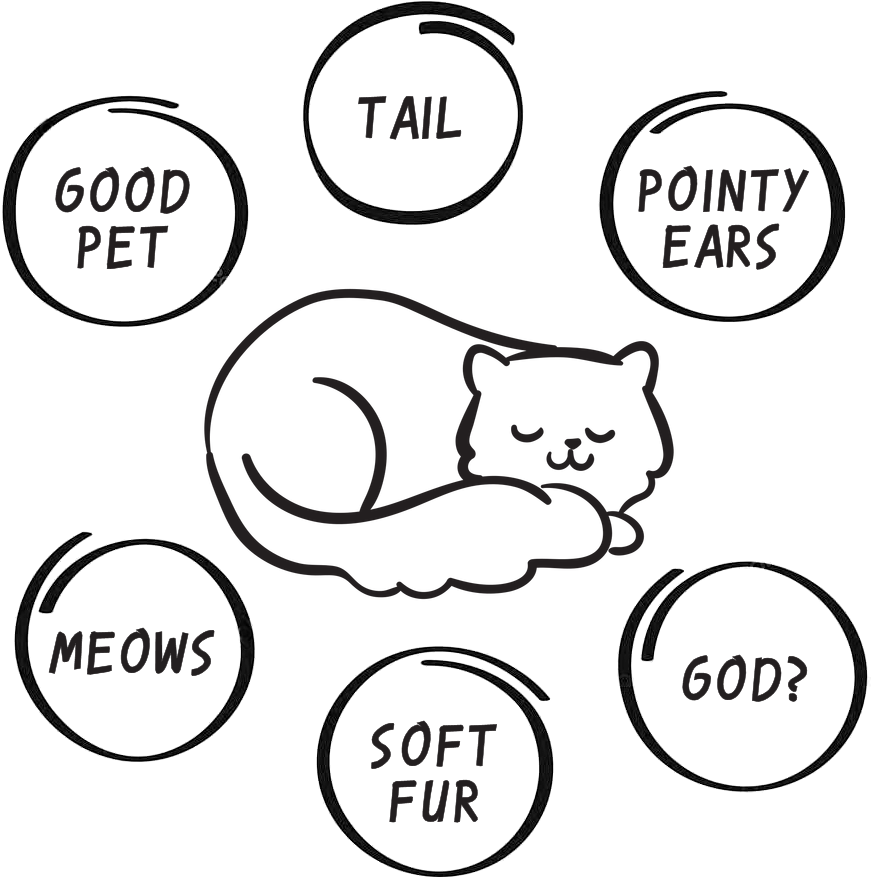
\includegraphics[width=0.6\linewidth]{graphics/cat-intensions.png}
    \caption{Some simple intensions for \textit{``Cat''}.}
    \label{dog}
\end{figure}

\subsection{Connotation}
Many words have an associated emotional colouring, which they have gained through social context and usage. For example, you could describe a person as \textit{slim}, \textit{thin} or \textit{scrawny}. While each of those adjectives describes less body fat than the expected average, they all clearly convey slightly different value judgements. Slim is often associated with attractiveness, thin is neutral, and scrawny is verging on the offensive.

\subsection{Word Sense}
Word sense can be thought of as a word's complete meaning in its entirety. It encompasses any possible reference and denotation; it includes the full set of intensions with all of their associated connotations. Describing a word's sense is often useful when distinguishing between different sets of intensions that could belong to a specific term. For example, the term \textit{``Cats''} has at least four different word senses:

\newpage
\begin{enumerate}
	\item Feline mammals
	\item The Andrew Lloyd Webber musical
	\item Jive talking jazz musicians (1920s slang)
	\item Catalytic converters
\end{enumerate}

Sense 1 and Sense 2 are related, but they are quite distinct concepts (The musical is about, and named after, the animals). Sense 1 and Sense 3 are also etymologically related; jazz musicians have sharp reflexes and are alleged to always land on their feet. Whereas Sense 4 shares no relation with any of the other three, the fact that it too can be referred to via the word ``cats'' is a mere linguistic coincidence, an evolutionary convergence of form. Cat the mammal has historical roots in Proto-Germanic: \textit{``catte''} meaning cat, and catalytic derives from the Greek word \textit{``katalusis''}; Transliterally: \textit{``before-decomposition''}; Translated: initial or initiating action (catalyst).

The meaning of the word \textit{``meaning''} is nebulous, so I will avoid using it where possible. Instead, we will be favouring the more precise word \textit{sense} or \textit{word sense}. All words and terms have an associated word sense unless they are nonsense words, then they, of course, have no sense\footnote{I was delighted to discover the same joke in Wittgenstein's book \textit{Tractatus Logico-Philosophicus} in German. I guess \textit{``great minds think alike"} or rather \textit{``Zwei Dumme, ein Gedanke"}.}.

\subsubsection{Word Definition}
A word's definition is a precise sense, handcrafted by experts for domain-specific nomenclature. The one we are taught in primary school is the biological taxonomy, but every field and activity has its own nomenclature. The word ``brush'' will have a different sense when spoken by a painter, a hairstylist, a makeup artist, a dentist, or an electrical engineer. But they all understand the difference between ``paintbrush'', ``hairbrush'', ``makeup brush'', ``toothbrush'', and ``carbon brush'' (A painter does not usually brush their teeth with a paintbrush). The nomenclature I use every day is that of spoken (and written) English, codified by lexicographers in general-purpose dictionaries. The dictionary is not a superset of all other nomenclatures. It too is domain-specific, the domain of common usage which entails all the idiosyncratic nuances of regional dialects.

A definition ---regardless of the nomenclature--- is carefully designed by experts to include only elements which are both \textit{necessary} and \textit{sufficient} to uniquely identify it. Almost 2,500 years ago, Plato attempted to create a universal definition for ``human''\footnote{Human: The animal who is always in heat.}, which was \textit{``a featherless biped''}. The next morning at the Platonic Academy, Diogenes ---the original cynic and cheeky smarty-pants--- proclaimed \textit{``Behold, Plato's man!''} while holding a plucked chicken aloft. Proving Plato's definition was not sufficient. Featherless may be a necessary condition, but biped may not be as Oscar Pistorius the Blade Runner. The fastest man on no legs, is a human. Although some would argue he is not, not after what he did.
 
 %  usually relative to some context e.g.\ medical definition, biological definition, cosmological definition... the most common is the \textit{dictionary definition}, which is designed for the purpose of general usage, but is prone to the errors induced by ambiguity. 

%The biblical definition of \textit{Jesus} entails the necessary condition \textit{circumcised}, as someone who is not circumcused is necessarily not Jesus, however it's not a sufficient condition, because there are many people who are circumcised that are not Jesus.

%To be a Planet, it is necessary condition to be large enough to become spherical under one's own gravity. But It is not sufficient as Pluto is not a Planet. 

\section{Ambiguity}
If we return to our previous example, \textit{``I love cats''}, we can see that not only is nothing specific being referred to, but also exactly which word sense is denoted is not immediately obvious. Did the author intend to convey a love for the feline mammal, the musical, or some superclass encompassing both? The sentence is ambiguous. An ambiguous statement has two (or more) distinct and sharply precise interpretations. Natural languages are naturally ambiguous. English certainly is.

Ambiguity causes a confluence of senses. Under the term's lexical blanket, word senses may become merged. In this state, distinct words are mistaken for each other, which leads to miscommunication. Within IR research, this phenomenon is known as \textit{Term Conflation}. For example, all of the documents (or websites) containing the term \textit{``apple''} include documents on fruit with crisp flesh and documents about the iPhone company. So to be able to satisfy an information request accurately, a search engine needs to be able to discern the correct word sense for the term \textit{``apple''}, this is to disambiguate the word sense. This process is widely known as Word Sense Disambiguation (aptly named), a specific kind of semantic disambiguation.

\subsection{Vagueness}
Vagueness is often confused with ambiguity. It is, however, a distinct concept. An ambiguous sentence has several precise senses, whereas a vague sentence lacks even one precise sense.

\begin{center}
    \textit{``They will address this issue."}
\end{center}

That sentence is vague. Who is \textit{``they''} referring to? What is the issue? And how exactly will it be addressed? One can be unintentionally vague for many reasons; perhaps one lacks the vocabulary to articulate precise semantics. Or, sometimes, one can be intentionally vague. This is commonly seen in polite speech, where euphemistic phrases are used to avoid the vulgarity of objectionable words. There is also the real possibility of being \textit{Strategically Vague}, where one intentionally obfuscates what they are saying, to be evasive, or to avoid self-incrimination, like the rhetoric of politicians.

\section{Basic Sense Relations}
No word exists in isolation. Each word belongs to an ontology, an entire language, so we should consider how each word relates to all the other words within the language. We can consider the \textit{orthographic similarity} between words, which identifies the similarity of word spelling; the \textit{morphological similarity} considers the word's structure and formation, taking into account root words, prefixes, suffixes...; the \textit{phonetic similarity}, which considers how the words are pronounced. These comparisons encompass etymological derivation, tense derivation, among other more subtle distinctions. 

The most important relationship I am interested in \textit{semantic similarity}, which is known as the sense relation, how similar the respective word senses are, and how dissimilar they are (irrespective of spelling and pronunciation). This allows us to explicitly distinguish between the lexical form of terms from their semantic word sense to help accomplish our ultimate goal of word sense Disambiguation.

%The rest of this chapter is dedicated to the different kinds of identifiable sense relations, including the well known synonymy and antonymy, and also the seemingly less frequent but equally important generonymy and holonymy, as well as several others. 

\subsection{Structure of Sense Relations}

\begin{figure}[b]
    \centering
    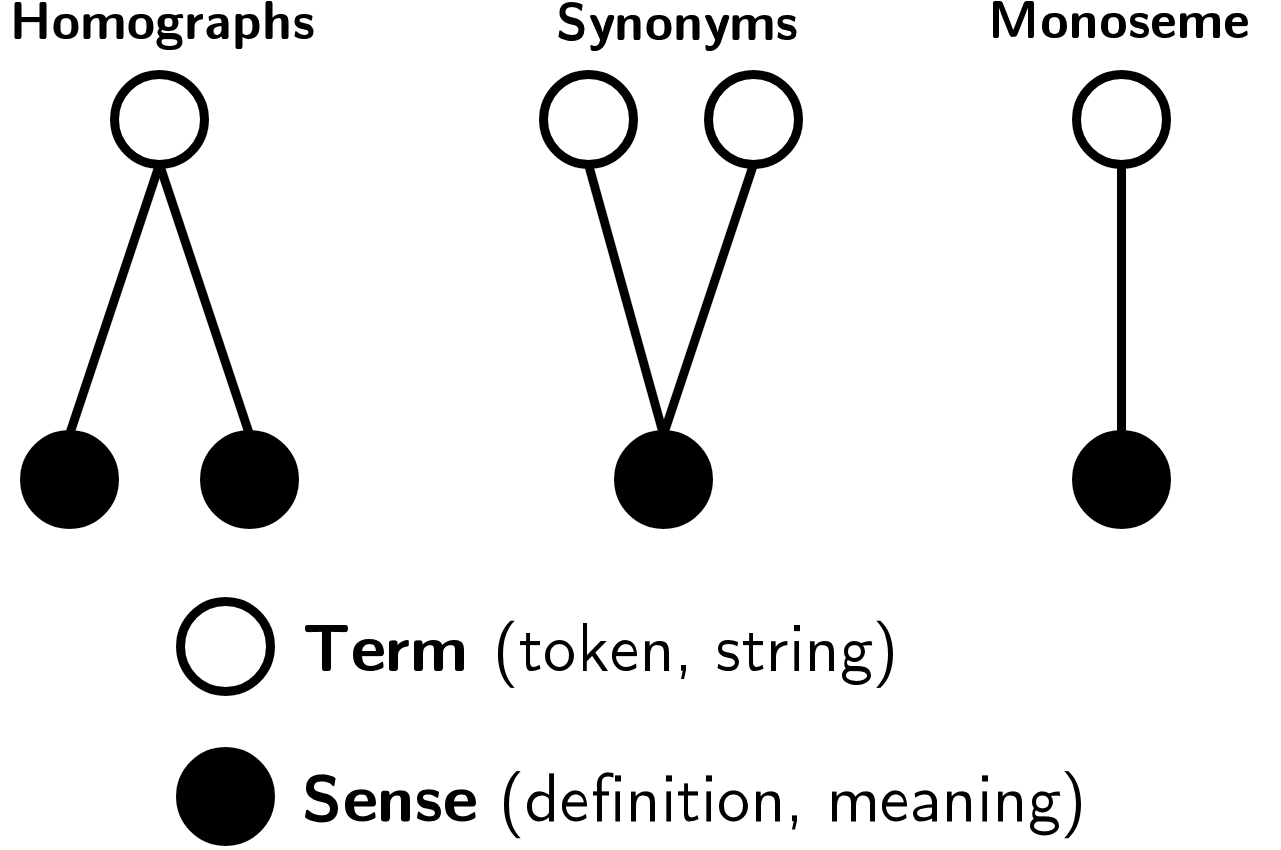
\includegraphics[scale=0.5]{graphics/sense-relations.png}
    \caption{The three basic sense relations.}
    \label{fig:sense-relations}
\end{figure}

% (``with name'')
% (``same name'')
% (``single name'')

There are three basic sense relations shown in Figure \ref{fig:sense-relations}, two of which can cause the plague of vocabulary mismatch. The first is synonymy (with name), where a single concept is associated with two or more different lexical words (e.g.\ ``big'' and ``large''). The second is polysemy (many names), where a single word is associated with two or more distinct concepts (e.g.\ ``cats'' and ``Cats''), The third, which does not concern us greatly, is monosomy (single name), where the concept is associated with one word, and that word is associated with one concept (quite rare), an example of monoseme might be ``\textit{aglet}''. If all words were monosemes, then semantic disambiguation would be trivial. Sadly natural languages were not designed with this in mind. Instead, languages are developed by discordant committees of recently domesticated primates.

%discordant ape like creatures.

\subsection{Homonymy}
Lexical ambiguity is the most simple kind of ambiguity, usually caused by homonymy (same name). We can distinguish between two main classes of homonymy, and in the context of this thesis, we can disregard homophony (same sound) and focus on homographs (same spelling). Homographs are words which have different sense but are spelled identically. Nobody would be surprised if I pointed out that trees, elephants, swimmers, and cars all have trunks because we all know intuitively that there are more things in this world than we have words for them.

\begin{center}
	\textit{``The pilot banked.''}
\end{center}

% My boss was horrified when I pushed my head into his trunks

The above sentence is ambiguous as ``bank'' could mean either an aeronautical manoeuvre or a financial transaction. Since both interpretations are equally valid, it's impossible to discern which single interpretation the author intended.

% \begin{center}
% 	\textit{``I was banking on the plane to bank into the river bank for I had over-insured it with my bank.''}
% 	\\ --- Antanaclasis Contrivance
% \end{center}

\subsection{Polysemy}
Polysemy (many meanings) refers to individual words having several distinct but related senses. It is similar to homonymy in general but differs where the different senses must have some shared association. The distinction between them is tightly linked, and oftentimes harder to spot the ambiguity.

\begin{center}
	\textit{``How to make a chicken salad. \\ Step 1: Make a salad. \\ Step 2: Give it to the chicken''}
\end{center}

The first occurrence of chicken in this sentence is initially ambiguous, referring either to the animal or the meat. This example is supposed to be humorous, and hopefully, you experienced mirth, not embarrassment, upon realizing you had been deceptively led down the garden path. The last sentence is incompatible with the initial interpretation of the first sentence. This forces a cognitive reinterpretation of the semantics. The ambiguity is simultaneously acknowledged and reconciled \textit{...your expectations were subverted, and from whence the humour arose.}\footnote{The young pedant R. Herring would say this after an unnecessary and tedious deconstruction of his own joke--- a despicably self-indulgent man.} %I cannot imagine any more insipidly self-indulgent behaviour.}

Here is a simpler example of the polysemy of \textit{``chicken''}:

\begin{center}
	\textit{``The chicken is ready to eat!''}
\end{center}

The above wordplay cannot be done with most animals in English, as there are usually distinct words for an animal's meat (e.g. beef for cow meat, pork for pig meat). Chicken, the live bird, and chicken the meat are related but clearly different senses. 

There are many different categorisations of polysemy, some more common than others, but all contribute to ambiguity and the vocabulary mismatch problem to varying degrees.

%Homonymy and polysemy aren't mutually exclusive, as shown in the following contrived 

\subsection{Synonymy}
% 
Synonymy (same name) is the relationship between orthographically distinct words that share the same or near-identical word sense. For example, ``big" and ``large" are synonyms, as they are spelled differently, and they share the same sense. Synonyms would be redundant in language usage if there were not more subtle nuanced distinctions that separate them. The degrees of similarity between synonyms are graduated, the most extreme being absolute-synonymy, which is where the words are perfectly identical, and the less extreme being parasynonymy (near name) and partial synonymy \cite{cruse1986lexical}.

\subsubsection{Absolute-synonymy}
Absolute-synonymy is quite rare since it is required that the words could be interchanged in \textit{all} contexts, their difference being only the orthographic spelling. Abbreviations and acronyms can be absolute synonyms, but ``big'' and ``large'' are not absolute synonyms because your \textit{``big sister''} is not the same as your \textit{``large sister''}.

%Which reminds me of this wonderfully understated joke: 

%\begin{center}
%\textit{``Ah, I tell you until I met my wife I always felt incomplete. Now I’m finished.''} 
%\\ --- Norm Macdonald
%\end{center}

\subsubsection{Parasynonymy}
These are words that appear to be absolute synonyms in one nomenclature but are polysemes in another. Mist and Fog are parasynonyms since, in common speech, they both denote a visible mass of condensed water vapour. However, in a meteorological context, there is a precise distinction between how the vapour is formed regardless of density, and the New Zealand Transport Agency makes a precise distinction between how much visual obscurity is caused regardless of the formation\footnote{In meteorology fog is descended cloud, whereas mist forms directly from a nearby water body. In transport safety mist is more transparent than fog, which is more opaque. High-beam headlights are ill-advised when driving through fog as the light reflects back at you.}. So only in common usage would it be appropriate to swap the words mist and fog.

\subsubsection{Partial synonymy}
Partial synonymy is when the similarity relation is not reflexive. That is to say, interchanging the words is only guaranteed to work in one direction. The words ``car'' and ``vehicle'' are partially synonymous because all cars are vehicles, but not all vehicles are cars.  ``Normal'' and ``proper'' are also partially synonymous. People often use those words as if they are interchangeable, however ``proper'' can be used as a pejorative, ``normal'' cannot. Normality is a provable and statistically verifiable state, whereas proper is a value judgement. You cannot label anything as proper just because it is normal.

\begin{table}[h]
    \begin{center}
    %\begin{table}[h]
        \begin{tabular}{|l|lll|}
        \hline
        \textbf{Word} & \multicolumn{3}{c|}{\textbf{Connotations}} \\ \hline
        Conscientious Objector & good & strong & passive \\
        Conchie                & bad  & weak   & passive \\
        Freedom Fighter        & good & strong & active  \\
        Pacifist               & good & weak   & passive \\ \hline
        \end{tabular}
    %\end{table}
    \end{center}
    \caption{The social connotations of anti war}
    \label{tab:psycholinguistic-connotation}
\end{table}

Oftentimes the only discernible difference between synonyms is the social connotation, where the distinction only matters in situations where there is an expected level of politeness or formality, e.g.\ one could describe another who breaks the law as a ``felon'' or a ``crook'', but it would be inappropriate for a Court Magistrate to refer to anyone as a crook in court\footnote{Unless in an unfortunate case of nominative determinism their name was actually ``Crook''}. The connotation entails all the wonderful nuance, the subtle undertones of political and social intention. According to psycholinguistics, words can be connotated in three primary dimensions: Good \& Bad, Weak \& Strong, Active \& Passive \cite{osgood1957measurement}. See Figure \ref{tab:psycholinguistic-connotation} for an example.

The connotations of some the terms in Figure \ref{tab:psycholinguistic-connotation} have evolved over time and are relative to one's own individual political sensibilities. Even seemingly agreed-upon words like ``cat'' can still have a variety of connotations. This is obvious when considering cat lovers against someone who is allergic to cats. The denotation is still the same mammal (e.g\ four legs, whiskers, pointy ears), but the connotation can be quite different.

%Cognitive synonymy

\subsection{Antonymy}
This is one of the more well-known sense relations since it is taught at the primary school level. An antonym (against name) is conventionally thought of as a word whose sense is contrary to another. For example, the words ``left'' and ``right'' are opposite directions so are antonyms of each other. Many antonyms exist on a single dimensional spectrum between two extremes, (e.g.\ \textit{hot, warm, tepid, cold, freezing}). These are known as gradable antonyms. Complementary antonyms have no degrees of gradability but usually express mutually exclusive binary states like ``alive'' and ``dead'', or ``fictional'' and ``factual''. Relational antonymy describes relations between concepts, usually derived from a hierarchy where we have converse pairs like ``boss'' and ``employee'', ``husband'' and ``wife'', or ``parent'' and ``child''. Things get tricky when considering different dimensions an antonym could take from a single word. Is the antonym of ``uncle'' the word ``auntie'' or ``nephew''? Well... both, it depends on the context, whether we are exploring the gender dimension or the ancestral dimension. 

% evening morning
% horizontal vertical

%They are not so easy to group into antonymous pairs, like ``hot'' and ``cold''
%Sometimes these spectrum's have obvious limitations, and sometimes 

% Complementary antonymy each sense is relative to the other, and oftentimes each sense is defined in terms of the other. 

% Interdependence. 

% Unity of opposites. 
% One cannot exist without the other, but they're not strictly contrary.

% material and immaterial
% moral and immoral
% right and wrong
% normal and abnormal

% Parent and child
% Employer and employee
% Teacher and student
% Buy and sell
% Husband and wife
% Predator and prey
% Perpetrator and victim
% Offense and defense
% Slave and master

% politician civilian
% liberal and conservative
% atheist and religious

% chemical and natural
% fictional and factual
% science and supernatural

% Fragile and Robust

% Antifragile


\section{Morphological Changes}

Synonymy and polysemy are the two obvious causes of vocabulary mismatch, but there are a few others we should be aware of that also cause vocabulary mismatch. A word can take many forms, including: tense, case, voice, aspect, person, number plural, gender, and mood. Linguists categorize the different types of morphological change as inflection, derivation, conjugation, and declension. While different word forms are not usually considered synonyms in the conventional sense, through the eyes of a machine, the different forms are orthographically distinct while the sense is very similar. For example, the word sense of ``cat'' is nearly identical to ``cats''.

% When undergoing morphological change the word sense does not change (or only mildly) so these different word forms can be seen as a form of synonymy.

\subsection{Pluralisation}
A word can be inflected to indicate number with either the suffix `s', `es, `ies', or various irregular exceptions. Google's analysis on user behaviour has discovered that in the context of web search, a plural form often indicates whether the user intends to purchase something online \cite{david2006google}, which does make some sense. If the search query was ``digital camera'', the user is likely interested in the concept denoted by \textit{digital camera}, how they work, what they look like, etc. Whereas if the query was ``digital cameras'', it is more likely that the user would be interested in several different types of digital cameras, possibly to compare a variety of them, possibly to determine which kind might best suit their specific needs. That is to say, we can infer that if they need a camera, they might want to purchase one. However, such a long chain of assumptions weakens the inference. Regardless of the justification, plurals can be used to infer what the user's \textit{information need} might be.

% \subsbusection{Inflection}

% inflected forms

% properties or relational information

% present tense, past tense, past participle, and present participle

% Here we added a suffix a very common way to inflect words in English.

\subsection{Derivation}
Derivation is a type of inflection that changes a word's lexical category. One can derive an adjective from a verb, for example ``joyful'' from ``joy''. One can also derive nouns from a verb: ``song'' from ``sing''. In the previous example, a vowel was changed, although changing the suffix is the most common way word derivation occurs.

\subsection{Conjugation and Declension}
Conjugation refers to verb inflection (verb tenses). Languages can have many complicated conjugation rules, especially when accommodating irregularities. Declension is the inflection of everything else, nouns, pronouns, adjectives, determiners etc. Declining a word does not change the lexical category. English only declines nouns to make plurals and also pronouns. German, however, has very complicated declension rules for many words: nouns, pronouns, articles, adjectives, for number, gender, and case.

\begin{center}
\textit{I would rather decline two drinks than one German adjective.}
\\ --- Mark Twain, The Awful German Language
\end{center}

\subsection{Spelling Variation}
An example of absolute synonymy is spelling variation. For example ``colour'' and ``color'', or ``yogurt'', ``yoghurt'', ``yoghourt'', and ``yogourt'' (and when combined with inflection, there are dozens of yogurt variations). Many arise from regional dialects, but on the multicultural, English speaking side of the internet, all of these forms are possible and accepted, which is also useful to know if you are an aspiring internet spelling bee champion.

% indexing process minimal processing, i.e. conversion to lower case, or spelling normalisation

% \subsection{Metaphor}
% Figurative language is common in the poetic arts. When Shakespeare called the world a stage, he did not mean literally but rather figuratively. We would not expect a search query to be written in poetic language. However, metaphor is pervasive in speech, the \textit{foot} of a mountain, the \textit{mouth} of a river. In the world of computing, we commonly use the metaphorical words: \textit{Bootstrap, Branch, Bug, CamelCase, Daemon, Motherboard, Nibble, Pipe, Reboot, Seed, Semaphore, Syntactic sugar, Tree, Trunk, Zombie}. The \textit{World Wide Web} itself is a metaphor for a spider's interconnected web. Within the internet, we also have: \textit{Bookmark, Cloud, Crawler, Firewall, Gateway, Mailbomb, Portal, Surfing}, and the undesirables of the web: \textit{Spam, Trojan, Virus, Worm}. The entire computer user interface is rife with metaphor: \textit{Mouse, Desktop, Clipboard, Attachments, Buttons, Files, Recycle bin, Wallpaper, Windows, Wizard, Zip}. I would also argue that: \textit{Hub, Queue} and \textit{Stack}, are used more figuratively than literally, but that is beside the point. The point is that metaphors sneak into our language far more frequently than we are usually aware of, about once every ten seconds \cite{geary2011other}. However, many of the previous examples would be considered \textit{dead metaphors} rather than the \textit{fresh metaphors} found in poetic prose.

% \subsection{Metonymy}

% Metonyms (change name) are used as replacement words. They refer not to the usual concept but rather some other distinct but associated concept. For example, we might call a New Zealand citizen a ``kiwi'', though they are not literally a flightless bird. \textit{Kiwi} (the bird) and \textit{kiwi} (the people) are polysemous.

% \begin{center}
% 	\textit{``How to make a kiwi salad: \\
% 	Step 1: Make a salad. \\
% 	Step 2: Add kiwi fruit. \\
% 	Step 3: Give it to a kiwi''}
% \end{center}

% The word \textit{Kiwi} (the people) and \textit{New Zealander} are partially synonymous with each other. We should always be aware that a sense relation between words does not exist independently but rather is interwoven within the fabric of language.

% A common basis association in metonymy is \textit{contiguity}, which is when the replacement concept frequently co-occurs with the replaced concept, e.g. kiwi birds, and kiwi people both originate in New Zealand. Other associations which underpin metonymy include metaphor, analogy, visual resemblance and also ellipsis. New Zealand citizens share no salient features with the Kiwi Bird, so referring to them by the metonym ``kiwi'' is not metaphorical or analogical resemblance.

% \subsection{Proper Nouns}
% Metonymy is especially prevalent when referring to a specific referent: \textit{a person}, \textit{place} or \textit{thing}\footnote{but what is a place? but a thing large enough to stand on, and what is a person but a thing that can talk back.}. Some \textit{things} become so widely known that they gain an epithet, an attribution provided after the standard name, as in Alexander \textit{the Great}. Antonomasia is when the phrase excludes the referent's standard name, e.g.\ ``The King of Pop'' or ``The Big Apple'', i.e.\ a metonym. Antonomasia also includes aliases, pseudonyms and nicknames like ``George Orwell'' being the pen name of ``Eric Arthur Blair", ``Father of Computer Science'' referring to the great Alan Turing.

%, or ``Laughter Critic'' referring to Plato\footnote{Plato thought laughter to be an irrational emotional outburst. He also thought laughing itself to be evil, to take delight in an other's self-ignorance --- and that malice is morally objectionable}.

% Many of us understand these metonyms intuitively; they are, after all, used primarily for famous referents. And if we are unaware of some specific nickname, there is certainly someone nearby who can help elucidate these for us. A machine has no such affordance.

%The distinction between homonymy and polysemy becomes blurred henceforth
%Not strictly a kind of polysemy, although we are still discussing words with related senses.

% \subsubsection{Eponymy}
% An eponym is a proper noun named after a specific historical person or region, usually the person who discovered or invented the noun's referent or region of origin. Common things which are eponymously named include body parts, diseases, laws, and food.

% \begin{center}
%     \textit{Moore's Law, Zipf's Law, Turing Test}
    
%     \textit{Reuben Sandwich, Roman Numerals, Champagne...}
% \end{center}

% And since proper nouns can be legally copyrighted, we can now distinguish whether a referent is legally authentic or a cheap imitation. Is sparkling wine made \textit{via methode champenoise} but outside of the Champagne wine region even real champagne? Are Roman numerals written outside of Rome even real numbers? 

% \subsubsection{Generonymy}
% Legally trademarked names are frequently used out of their legal context, to the point at which they lose their legal definition. This is known as Trademark erosion. When searching for something on the internet, we often use the verb ``google'', we refer to inflated cushioning as ``Bubble wrap'', and my mother will never not refer to any video game console as ``the Nintendo''. Sometimes these words become so common in speech they become considered generic. It is possible that the trademark protection will be legally dropped, as in Motorola's previous trademark ``Flip Phone'' or Apple's ``App''.

% the Lego company trying to enforce the plural form is lego not legos 

%Referring to a plush toy as a cat, is a kind of ..., the reference is through resemblance, a kind of visual metaphor. The soft toy still shares many salient or prominent features with cats.

\section{Ontological Relations}

So far we have only discussed attributes of a word and binary relationships between words. However, words do not exist independently but rather interwoven within the fabric of language, so let us quickly discuss hierarchical relationships and indirect relationships before moving on to the next chapter.

\subsection{Meronymy and Holonymy}

Objects in the real world can be broken down into constituent parts, and sometimes we might refer to the whole of an object from one of its parts. For example, a car could be referred to simply as ``wheels''. This is known as meronymy (part name), a specific type of partial synonymy. This language feature is often used to shift the reader's focus to what is most relevant for the situation. For example, if I had to feed several hungry people, I might refer to them as ``mouths'' to feed. There are several ways in which something could be considered a part of something else. Table \ref{meronymyholonymy} shows the most common types.

% \begin{center}

\begin{table}[h]
\centering
\begin{tabular}{|l|l|l|}
\hline
\textbf{Type}  & \textbf{Meronym}   & \textbf{Referent}    \\ \hline
Structure      & wheels  & Vehicle with wheels \\
Characteristic & fizzy   & Carbonated beverage \\
Substance      & ice     & Cube made of ice   \\
Containment    & wine    & Glass filled with wine \\ \hline
\end{tabular}
\caption{Different types of Meronyms}
\label{meronymyholonymy}
\end{table}

% \end{center}

%Containment     Pint            Pint of beer
%Membership      Otago Daily Times	a person who works for the ODT

The inverse of meronymy is holonymy (whole name), which occurs when denoting or referring to a constituent part from its whole. For example, being ``interviewed by the Otago Daily Times'' does not mean the entire company conducted the interview, more likely by a single employee or representative. 

% Perhaps this is an elliptical expression, or possibly both?

%Some examples of meronymy or holonymy may be caused by ellipsis. We do not care so much how the language evolved each particular phrase, but rather how they relate to each other now.

\iffalse
Wheels	    Car						            Part			precise
Blade		Sword						        Part			precise
Boots		Soldiers					        Part			precise
Toast		toasted bread					    Part			precise
Fizzy 		carbonated beverage				    Part			precise
Bubbly		sparkling wine					    Part			precise
Redhead	    a person who has red coloured hair		Part	    precise
Suit		a business person who wears a suit		Part		precise
Glasses	    spectacles made of glass			Substance		precise
Rubber	    Latex rubber condom				    Substance		precise
Ice		    ice cubes					        Substance		precise
Chalk		Stick of chalk					    Substance		precise
Paper		newsprint paper
\fi

\subsection{Hypernyms and Hyponyms}

We can categorize words by their degree of specificity and generality. In information science, an ontology is a structured hierarchy identifying categorical relationships between concepts, a taxonomy of words. The top-level or root of any ontology is the most general and includes more schematic or abstract concepts. The lower levels include more specific and detailed concepts or instances. This kind of data structure should be reminiscent of the knowledge base representations mentioned earlier and our mental model of word associations.

%The intermediate levels are 

\begin{figure}[h]
    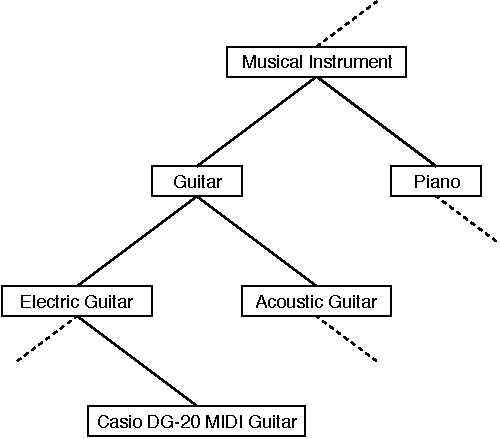
\includegraphics[width=0.8\linewidth, left]{graphics/level_of_specificity.pdf}
  \caption{Simple Ontology Example}
  \label{fig:ontology}
\end{figure}

\iffalse
\begin{table}[h]
\begin{tabular}{|l l|}
\hline
Physical object & \textit{Most generic} \\
Musical instrument & \\
Guitar & \\
Electric Guitar & \\
Casio DG-20 MIDI Guitar & \textit{Most specific} \\
\hline
\end{tabular}
\end{table}
\fi

The level at which we refer to something is strongly dependent on the current context. When in a music shop, it would be important to distinguish \textit{precisely} which musical instrument you might refer to. But when in my bedroom you may be more general, as ``the guitar'' could only refer to my 3/4 size acoustic guitar that I bought, fully intending to learn how to play it one day. The convention is to adhere to the Level of Usual Utility \cite{brown1958shall}, one should not be annoyingly vague nor cumbersomely explicit. One should convey strictly enough information for the situation. If one were looking on the internet to purchase a guitar, the level of specificity would be important.  

%Superordinate level
%Intermediate level
%Suborinate level
%superordinate,


%hierarchical structure

The categorical relationships described above are known in linguistics as hypernymy and hyponymy. A hypernym (over name) refers to a more general term, and a hyponym (under name) refers to a more specific term. This is another kind of partial synonymy we mentioned earlier. It is sometimes considered a \textit{type-of} relationship, distinct from the other class of partial synonymy (meronymy and holonymy), which are considered a \textit{part-of} relationship. Another distinction is that Hypernymy and Hyponymy are transitive relations, so if a Casio DG-20 is a type of guitar, and a guitar is a type of musical instrument, this allows us to infer that Casio DG20 is a type of musical instrument by the rule of transitivity.

In everyday speech, one might make a breakfast request of \textit{``eggs on toast with a glass of milk''} from a caf{\'e}, and a maliciously compliant genie who works at the caf{\'e} could serve \textit{fish eggs} and \textit{giraffe milk}. The breakfaster likely intended \textit{chicken eggs} and \textit{bovine milk} as they are the most commonly egg and milk products consumed in our society, which is why we can refer to them through their respective hypernyms ``milk'' and ``eggs''. Academics and suits of marketing tend to use hypernyms to make products sound more sophisticated than they actually are. For example, a toothbrush might be referred to through its hypernym ``dental cleaning tool'', or even calling a web search engine a ``digital information retrieval system''. Such a level of over-specificity is redundant and prevents clear and concise communication.

Now that we have established an understanding of how words relate to each other within an ontology in the next chapter we will investigate various methods of modifying search queries to improve document retrieval. The method we are most interested in are those which use a semantic ontology to inform this modification process.
        \chapter{Improving Search Queries}
\begin{flushright}
    \textit{``Anything worth knowing is worth writing down."}
    \\ --- bullseyed723 (reddit.com 2016)
\end{flushright}


% A Survey of Automatic Query Expansion in Information Retrieval
% https://dl.acm.org/doi/pdf/10.1145/2071389.2071390


%%%%%%%%%%%%%%%%%%%%%%% link language back to vocab mismatch
In the previous chapter, we established a fairly comprehensive foundation of how words can be conflated. We can apply that knowledge to try and improve search queries from a linguistic perspective. Vocabulary mismatch (term mismatch) in ad-hoc retrieval is caused by document authors and query authors not using the same words, primarily caused by natural languages' highly ambiguous nature. An obvious cause of term mismatch are morphological differences, for example, ``teacher'' and ``teaching'' both derive from the same root word ``teach'', they both refer to the same concept, but a term matching system will fail to infer any relevance as they are clearly distinct terms. The two main causes of vocab mismatch (i.e. lexical-semantic differences) are synonymy and polysemy. If a query and document use \textit{different} terms but the same word sense (synonyms), the term matching system could fail to retrieve a relevant document (false negative) and consequently reduce recall. If the query and document use the \textit{same} terms but with different intended word senses (polysemes), the term matching system could retrieve the non-relevant document (false positive) and consequently reduce precision. \textit{Recall} and \textit{precision} are retrieval performance metrics. A comprehensive explanation of recall and precision can be found in Chapter \ref{chap:experiment-conditions}.

%%%%%%%%%%%%%%%%%%%%%%% QUERY REFORMULATION
\section{Query Reformulation}
Query reformulation is the process of modifying a query into one which better represents the information need or one with a more useful vocabulary. During a search session, if a user is unsatisfied with the retrieved documents, they will often manually reformulate their query several times. Unfortunately, users can lack domain-specific knowledge and awareness of the vocabulary used in the document collection, which prevents ideal refinement. They may also lack the patience or persistence to refine the query until perfection, which is why this task is often outsourced to machines that are always faster and sometimes more effective.

Automatically modifying a user's query to improve retrieval performance was first suggested in 1960 \cite{maron1960relevance}. While early attempts were ineffective modern attempts are much better and can be found in many commercial retrieval systems. In modern web search, query reformulation happens before the first tier of a multi-tier ranking pipeline; the stage that reduces billions of documents to millions. Since the effects of query reformulation will propagate throughout the entire pipeline it is vital that queries are modified for the better. Much like baking a tasty cake requires quality ingredients, so too do the upper tiers of a ranking pipeline require high quality input.

The most common automated reformulation operations are appending, removing, and substituting query terms, but also re-weighting existing query terms to adjust their influence. Another reformulation operation (that is less relevant for our research) is the inclusion of refinement directives such as publication date, language, document type, origin. Appending terms to the query is the most common and most relevant reformulation to our research. It is known in the literature as \textit{query expansion}.

% There are several automated methods which can reformulate an inadequate search query. 
% Some are fully-automated and happen without the users knowledge, others are user guided and take direct input from the user to guide the reformulation.


%%%%%%%%%%%%%%%%%%%%%%% IQE
\subsection{Interactive Query Refinement}
The most apparent automated reformulation technique is Interactive Query Refinement, where a system provides suggestions to refine the query. The most well known is Google Suggest (the \textit{``did you mean...''} feature), which is very effective at refining a query if a user misspells terms. Google also has Autocomplete, which is a predictive text language model that suggests query terms to add. Another way a user can refine their search is with category filtering. For example, on Google Web Search, you can refine your search by selecting Images, Videos, News, Maps, Books, Shopping, etc. What unifies these different types of interactive query refinements is that the user has direct control. They judge whether the query would be better with or without the proposed reformulation.   



%%%%%%%%%%%%%%%%%%%%%%% AQE

% Regardless of the method of query expansion it has proven effectiveness in many domains TREC, biomedical datasets \cite{rivas2014study}, 

\section{Automatic Query Expansion}
The process of adding more terms to a query is called Query Expansion, and the purpose is to broaden the query's vocabulary to over come any vocabulary mismatch. The hope is to increase the likelihood that the query will contain terms that are also contained in the relevant documents while still capturing the user's information need. Automatic Query Expansion (AQE) can even be done without the user knowing it is happening.

A retrieval system can expand a query to compensate for any ambiguity. For example, if a search query contained the acronym (\textit{``IR"}), it could add the expansion of that acronym (\textit{``Information Retrieval''}) to the query, which would then allow the retrieval of a document that does not include  ``IR'' but does include \textit{``Information Retrieval''}. The first result on Google when searching ``IR'' (for me) is the New Zealand Inland Revenue Department's website, which does not appear to include the acronym ``IR''. This does not prove that Google performs query expansion. However, they apparently own 329 patents that mention ``query expansion'', which suggests they probably are. See Appendix \ref{appendix:googlepatent}. The number 329 could be an overestimate because I used Google's search engine to retrieve that list, and since it probably performs query expansion there's no guarantee that all those documents contain the phrase ``query expansion".

%%%%%%%%%%%%%%%%%%%%%%% stemming
\subsection{Stemming Methods}
There have been many attempts to perform query expansion using linguistic knowledge over the years, starting in the 1960s with stemming. These systems account for morphological differences by stripping suffixes from words. For example, \textit{``teacher''} and  \textit{``teaching''} would both be treated as the affix \textit{``teach''}. Suffix stripping systems of the 1960s-1980s include Lovins \cite{lovins1968development}, Porter \cite{porter1980algorithm}, Dawson \cite{dawson1974suffix} and Paice \cite{paice1990another}. These lexical systems account for most regular derived and inflected forms; however, they may preclude irregular forms like ``taught''. They may handle\MarkText[red]{``teached''} perfectly well, but it's very uncommon and is considered grammatically incorrect by most authors. 500 years ago\MarkText[red]{``forgat''} and \MarkText[red]{``digged''} were the preferred past tenses.

There are also many words that share morphology but share little semantic similarities, e.g. \textit{``awful''} and \textit{``awesome''} both derive from \textit{``awe''} but differ substantially in meaning. We could manually build a database to handle the thousands of exceptions in the English language, or we could apply statistical modelling to handle them automatically. From the 1990s we started to see statistical analysis (and later machine learning) used for stemming. Corpus-based co-occurrence analysis \cite{xu1998corpus}, Hidden Markov Models \cite{toman2006influence}, YASS  \cite{majumder2007yass}, Krovetz \cite{krovetz2000viewing}, and Xerox \cite{grefenstette1996detailed}. Unsurprisingly these statistical models are provably better in IR applications, especially when used in conjunction with suffix stripping \cite{jivani2011comparative}.





%%%%%%%%%%%%%%%%%%%%%%% statistical methods
% https://link.springer.com/content/pdf/10.1007/s10115-018-1269-8.pdf
% 2018 A survey of statistical approaches for query expansion

% https://link.springer.com/content/pdf/10.1007/s10115-018-1269-8.pdf
% 2017 survey
\subsection{Statistical Methods}

% Statistical analysis and machine learning methods can discover the presence of lexical-semantic relationships between words faster than humans but they struggle to identify exactly which linguistic relationship they find. 

% Language modelling has been applied to automatic query expansion problems with success  \cite{Bai:2005:QEU:1099554.1099725}. Usually no term semantics are explicitly used, only co-occurence data mined from the corpus. Some recent experiments however have begun to include term relationships  \cite{Bai:2005:QEU:1099554.1099725}.

% Term clustering Harper and van Rijsbergen 1978, Lesk 1969, Minker et al 1972

% \section{Clustering}
% scatter gather early 1990s  \cite{scattergather}
% documents can be clustered into semantic topics
% iterative process of identifying relevant topics, then gathering them into a larger cluster

Statistical methods expand a query by adding expansion terms that frequently co-occur with the original query terms in other text collections. These systems assume that if a statistical association is found, there must also be some linguistic association. They could be morphological derivations, synonyms, or potentially disparate concepts often used in the same context. For example, ``miracle'' and ``god'' are not synonymous but often co-occur in documents. These systems assume that documents that include the word ``God'' would be relevant to documents that include ``miracle'' and vice versa. This example is a huge oversimplification for explanatory purposes. 

These systems build a statistical thesaurus, then use the thesaurus to expand a query with the statistically associated terms. There are various ways to construct a statistical thesaurus, usually by performing co-occurrence analysis on the document collection \cite{jing1994association}. One could cluster the document collection first then build the thesaurus \cite{crouch1992experiments}. Or one could represent terms and documents as vectors and perform linear algebra to find associations \cite{qiu1993concept}. 

All of the previous methods source expansion terms from the document collection itself, which is why they are often called collection dependent in the literature. Some research suggests that an independent data source (i.e. an ontology) is better suited for bridging the vocabulary disparity \cite{biswas1986knowledge}. However, if a document collection is sufficiently large and contains content relevant to the query, then collection dependent methods are sufficient \cite{bhogal2007review}. Some pure statistical methods exist, but they are usually hybridized with another approach \cite{raza2019survey}, e.g.\ stemming or semantic methods.





%%%%%%%%%%%%%%%%%%%%%%% semantic methods
% A Taxonomy and Survey of Semantic Approaches for Query Expansion
% https://ieeexplore.ieee.org/stamp/stamp.jsp?tp=&arnumber=8625452
% A review of ontology based query expansion
% https://reader.elsevier.com/reader/sd/pii/S0306457306001476?token=AB893A4C1E9666FAC33030FA226694AA4798E8E805FDFD0877C45C284346EFB6B6C0C1C33E8C910A4F0F666B4F55AEF8&originRegion=us-east-1&originCreation=20210524085417

% https://citeseerx.ist.psu.edu/viewdoc/download?doi=10.1.1.227.7491&rep=rep1&type=pdf
%2004 A Study of Ontology-based Query Expansion

% 2019 Query Expansion Techniques for Information Retrieval: a Survey
% https://arxiv.org/pdf/1708.00247.pdf
\subsection{Semantic Methods}
Stemming is a purely lexical approach, and while lexical similarity often correlates with semantics, it is insufficient to capture the full semantics of a language. Semantic approaches aim to build complete taxonomies of word meaning, often called knowledge structures. These semantic models can vary in complexity from a simple thesaurus to an ontology. The distinction between an ontology and a thesaurus is not clear, but what they have in common is they associate pairs of words that share some semantic meaning. 

The most influential English thesaurus was constructed manually by Peter Mark Roget in the 19th Century. The first edition of Roget's thesaurus (1852) contained 15,000 words, an extraordinary feat. Manually building a knowledge structure by hand is prohibitively expensive since it requires hiring experts with domain knowledge of the documents. Despite their expense, some do exist, such as the Unified Medical Language System (UMLS), which contains terms from 40 biomedical vocabularies \cite{pmid27668467}, and has been applied successfully to IR tasks \cite{pmid9452981}.

Another approach to acquiring a thesaurus is with statistical analysis \cite{qiu1993concept}. However, these are not strictly semantic in nature. These statistical thesauri cannot guarantee that their associations carry any semantic information, only statistical, a distinction often omitted in the literature.

The most comprehensive linguistic ontology is WordNet (or EuroWordNet), a hierarchically organized lexical-semantic mapping table. The first version was constructed by Miller and his team at the Cognitive Science Laboratory of Princeton University \cite{Miller:1995:WLD:219717.219748}. The sense relations in WordNet are more precisely categorised than Roget's single binary category. In its entirety, WordNet is a vast interconnected ontological graph that connects over 155,000 distinct words to each other through 117,000 different concepts.

% General purpose 
% Roget, WordNet, EuroWordNet,  Cyc
% which are manually constructed. 

We can perform query expansion with a thesaurus/ontology by adding terms with the same or similar meaning to the query. Using synonyms from a thesaurus for query expansion makes perfect sense, as synonyms are the most obvious cause of vocabulary mismatch. Early IR research indicated general-purpose thesauri were effective \cite{ASI:ASI4630360102}, while later experiments proved their behaviour inconsistent. Sometimes they would significantly improve a query; other times degrade a query. Voorhees manually used WordNet to perform expansion and also concluded that it was too unpredictable to be useful in practice \cite{Salton:1968:CEI:321439.321441}. She said that lexical-semantic relationships provide little benefit but have the ``potential to improve an initial query'' \cite{Voorhees:1994:QEU:188490.188508}. She noted that poorly performing queries have a good chance of being improved but queries that already perform well tend to worsen when query expansion is applied \cite{mandala1998use}.

% Other semantic ontologies identify more categories than just synonyms, including hyponyms, ...

Some researchers found that using synonyms and hyponyms have a limited effect. However, using ``gloss words'' and ``common nodes'' had a better impact \cite{navigli2003analysis}. Here gloss words and common nodes are keywords that refer to broad categories.


% thesauri QE mixed results
% synonym expansion to be always useful
% hierarchical expansion only useful sometimes

%%%%%%%%%%%%%%%%%%%%%%% ISSUES

% It isn't clear if semantic methods have the capacity to improve search queries as are issues with reliability. The usual culprit blamed for degrading a query's performance is query drift, which we will discuss later.

% show that retrieval is improved if the user is aware query expansion is happening, and of the knowledge model being used  \cite{suomela2005ontology}  \cite{sihvonen2004subject}

%%%%%%%%%%%%%%%%%%%%%%% PROCESS AUTOMATION
% fully automated
% requires no user input to function
% fully-automated: (corpus based (psudo-relevance feedback), relationship based(thesauri, ontology))


% .Gonz-alo et al. (1998)use a manually disambiguated test collection of queries and documents derived from the SEM-COR semantic concordance. Their experiment covers three types of index spaces: original terms; word sensesderived from manual disambiguation and finally WordNet synsets. The authors observe that if queries are notdisambiguated, indexing by synsets performs only as good as standard word indexing. According to Gonzalo,indexing with word sense improves information retrieval by more than 29%.

% Relevance feedback described previously modifies queries with terms found in documents directly from the collection.
% , thus addressing any term mismatch directly from the collection's vocabulary itself.








%%%%%%%%%%%%%%%%%%%%%%% Relevance Feedback

% Relevance feedback sources new terms from the document collection itself, specifically from a subset determined to be relevant to the original query. Other query reformulation methods source new terms from external sources 

% explicit feedback - relevance judgements
% implicit feedback - top k assumed

\subsection{Relevance Feedback}
Relevance feedback is a query expansion technique that sources its query terms differently from the methods described previously. Relevance feedback modifies a search query with terms extracted from documents that are already known to be relevant. It modifies the query's vocabulary to be more similar to the relevant documents provided. It works by finding the content-bearing terms from the set of relevant documents; these terms best describe the relevant documents, i.e.\ they have a high term frequency but low document frequency. These content-bearing terms are ranked in descending order of importance, and the top terms in the rank are appended to the query. There may be hundreds of content bearing terms, but only a small proportion will be chosen to modify the query, which is why we must rank them and select the terms which have the best chance of improving the query. The query reformulation step may simply be appending the new terms to the original query and/or re-weighting the terms to adjust their influence in the relevance function. Setting their weight proportional to their content-bearing rank-score.

It is often implemented using Rocchio's algorithm \cite{rocchio1971relevance}, which was originally devised for the vector space model of relevance allowing for the intuitive explanation: move the \textit{query vector} towards the cluster of \textit{relevant document vectors}. There are many variations for implementing relevance feedback, including the Binary Independence Model (BIM) \cite{robertsonandsparckjones}, Chi-square \cite{article123}, Robertson selection value (RSV) \cite{Robertson:1991:TSQ:104889.104901}, and Kullback-Leibler (KL) divergence \cite{Carpineto:2001:IAA:366836.366860}. All essentially achieve the same goal: find the content bearing terms in the provided relevant documents and modify the query with those content bearing terms.

Relevance feedback can be very effective when adding term(s) relevant to the user's information need which the user unwittingly excluded. However, it can sometimes reduce the query's effectiveness if the provided relevant documents cover a variety of different topics and contain a variety of content-bearing terms, many of which are not relevant to the user's information need.

The obvious issue with relevance feedback is that it requires a set of documents that are known to be relevant to the user's query. This issue is solved by performing two separate searches. The first search finds the relevant documents, and the second search retrieves the final set of results. Early devisings of relevance feedback tasked the user with manually selecting these relevant documents. The search engine would first retrieve a set of documents with the user's original query; then, the user would indicate which documents are relevant using a binary or graded assessment. An improved version called Blind Relevance Feedback (or pseudo relevance feedback) removed the user from the pipeline by assuming the top documents from the first search would be relevant and contain the right content bearing terms. Blind Relevance Feedback is a fully automated system that can happen without the user even knowing it is happening. The biggest drawback to both of these relevance feedback implementations is that the time to search is doubled. You must perform at least two searches for every query, the first to acquire the set of relevant documents and the second to acquire the final set of results. Two passes through the search pipeline are especially slow in distributed search, requiring merging the documents lists from the first pass across a network \cite{martinezsantiago}. Despite its significant performance cost, Relevance Feedback remains one of the best query expansion approaches today \cite{Carpineto:2012:SAQ:2071389.2071390}.





%%%%%%%%%%%%%%%%%%%%%%%% ADDING TERMS...?
% one-third of the terms in the context of historical English text \cite{robertson1993comparison}.
\section{How many terms to add?}
Adding query terms can only increase recall; however, precision can go up or down depending on the quality of the expansion terms. There is no consensus on exactly how many terms should be added, as it depends on the query, the document collection, how the expansion terms are acquired, and where the expansion terms are from.

Some research indicates that adding 20 terms is optimal for relevance feedback systems \cite{harman1992relevance}. Some suggest between 300 – 500 terms for ``massive query expansion'' with collection dependent statistical analysis \cite{buckley1995automatic}. However, much research says there is no one-size-fit-all number as every query is unique \cite{billerbeck2004questioning} and that the type and quality of expansion terms is vastly more influential than the amount \cite{sihvonen2004subject}.





%%%%%%%%%%%%%%%%%%%%%%%% QUERY DRIFT

%It is possible that the ranking function will rank only about fruit higher than it would have before. 
%It is possible that one term from the original query may be over represented in the expanded query. 

\section{Query Drift} \label{sec:querydrift}
Query drift is often cited as the cause behind query expansion failure. Query drift is when the modified query's meaning has drifted too far from the user's information need. This happens if the expansion terms are not of good quality, i.e.\ they are not relevant, which is why we must choose the expansion terms carefully and not accidentally add spurious terms. The drift could be towards something specific but irrelevant or perhaps too vague to be helpful, especially if the system adds thousands of expansion terms.

\begin{table}
    \centering
    \begin{tabular}{|l|lll|}
    \hline
    Original terms  & fruit     & pie     & recipe      \\ \hline
    Expansion terms & apple     & crumble  & ingredients \\
                    & banana    & pastry  &             \\
                    & berry     & turnover &             \\
                    & blueberry &         &             \\
                    & juice     &         &             \\
                    & kiwi      &         &             \\
                    & lemon     &         &             \\
                    & orange    &         &             \\
                    & pineapple &         &             \\
                    & strawberry    &       &           \\
                    & watermelon    &       &           \\
                    \hline
    \end{tabular}
    \caption{Example expansion terms for the query ``fruit pie recipe''.}
    \label{table:querydrift}
\end{table}

Take the query: \textit{``fruit pie recipe''}. Table \ref{table:querydrift} shows 15 possible expansion terms which could be sourced from a semantic ontology, statistical analysis, or possibly relevance feedback. If we include all 15 expansion terms, then our modified query will contain 18 terms in total: 12 terms refer to fruit, 4 refer to pastry goods, and 2 terms are about cooking. If we use this modified query to retrieve documents, then a document that contains all 12 fruit terms will be ranked higher than a document that contains only the 3 terms: \textit{apple, crumble, recipe}, even though the latter document is almost certainly more relevant. The query has drifted towards fruit as we did not choose our expansion terms carefully enough.

Query drift is known to affect all the forms of query expansion discussed in this chapter. There are many approaches that attempt to deal with drift. In relevance feedback, drift can be mitigated by first refining the initially retrieved documents \cite{Mitra:1998:IAQ:290941.290995}. For co-occurrence analysis, accounting for the term proximity within the document can help alleviate eventual drift \cite{Xu:2000:IEI:333135.333138}. In the upcoming experiments, we will explore other ways one could reduce the effects of query drift.

% No matter which method is used, automatic query expansion is not perfect and will often append terms that cause query drift. 
% We will be using query expansion in order to improve the performance of queries.
% Clearly Query Reformulation can improve retrieval success, however we must be careful as to which words get added.
% chosen to explore lexical-semantic query expansion
% End chapter on how Query drift is our main concern
    
    \part{Experiments}
        \chapter{Experiment Conditions}
\label{chap:experiment-conditions}

The experiments herein will be focused on improving automatic query expansion using linguistic features, specifically reducing query drift. This chapter outlines the final few ingredients required to bake a tasty science cake.

\section{Search Engine}
The experiments will be performed on the academic search engine ATIRE \cite{Trotman:2012:OSI:2422256.2422269}, a bag of words term matching information retrieval system that ranks with an Okapi BM25 variant. The parameters of BM25 ($k_1$ and $b$) are chosen empirically by particle swarm optimization \cite{Trotman:2014:IBL:2682862.2682863} and are fixed for all experiments. The IDF component $log ({N} / {\mathit{df}_{\!\!t}} )$ from Robertson-Walker \cite{Lee:2007:IRS:1277741.1277891} will be used as it prevents negative weights. This is a useful feature for practical implementations because when the top-$k$ document scores are accumulated term by term, the scores will never decrease in value. Hence, documents that score 0 can be immediately discarded as irrelevant.

\subsection{Query Expansion}
BM25 ranking can be easily adapted to support na{\"i}ve query expansion (see Equation \ref{eq:bm24qe}) by modifying the query terms ($Q$) to include all expansion terms ($e_t$), Equation \ref{eq:bm25-expansion-terms}. More sophisticated expansion techniques will be introduced in the later chapters.

\begin{equation}
	Q_{e} \leftarrow \bigcup_{t \in Q} ( e_t \cup t ) ; \text{where } e_t \text{ is the set of expansion terms for } t.
	\label{eq:bm25-expansion-terms}
\end{equation}


%%%%%%%%%%%%%%%%%%%% REPLACE THIS BM25 formulation
\begin{equation}
	\text{BM25}(d) = \sum_{t \in Q_{e}} \: log \Big( \frac{N}{\mathit{df}_{\!\!t}} \Big) \times \frac{(k_1 + 1) \cdot \mathit{tf}_{\!\!td}}{k_1 \cdot \Big(1-b + b \cdot \Big(\frac{L_d}{L_{avg}}\Big) \Big) + \mathit{tf}_{\!\!td}}
	\label{eq:bm24qe}
\end{equation}

% \[
% 	\text{BM25}(d) = \sum_{t \in Q} \: log \Big( \frac{N}{\mathit{df}_{\!\!t}} \Big) \times \boxed{\frac{(k_1 + 1) \cdot \mathit{tf}_{\!\!td}}{k_1 \cdot \Big(1-b + b \cdot \Big(\frac{L_d}{L_{avg}}\Big) \Big) + \mathit{tf}_{\!\!td}}}
% \]

% \vspace{1em}

% \vspace{-0.3em}















\section{Expansion Terms}
% We used WordNet  \cite{Miller:1995:WLD:219717.219748} as a source of expansion terms.
Two data sets will be used as the source of expansion terms, and both are semantic ontologies that will be leveraged to address the vocabulary mismatch directly. The first is a modern edition of Roget's thesaurus, which identifies synonyms. We will use the 2004 Project Gutenburg edition, which identifies over 36,000 different concepts. 

% , and the most recent edition (2019) contains 443,000 words

The second ontology used is WordNet, which has a long history of use in language and information research \cite{fellbaum2010wordnet}. Over the years, WordNet has grown to include many more words than Roget's thesaurus, and account for many more language features, see Figure \ref{wordnet-history}. As mentioned previously, many IR researchers have used older versions of WordNet for query expansion, including Voorhees, who used version 1.3 \cite{Voorhees:1994:QEU:188490.188508}. We will use version 3.1, the most recent version currently available. We anticipate that using a modern version of WordNet will outperform earlier experiments as the literature says that successful query expansion depends on the quality of the ontology \cite{kim1990model, jones1993thesaurus}, i.e. coverage, completeness, and accuracy.

Apart from the number of included terms, the main point of difference between Roget's and WordNet is the classification of relationship types. Instead of having a single synonymous relation, WordNet has 25 different relationship types. Some are symmetric where the terms participating in the relation relate to each other in a \textit{SynSet} or \textit{synonym ring}. Other relationships are not symmetric and describe \textit{`is-a'} or \textit{`has-a'} relationships described earlier (holonyms, meronyms, hypernyms, and hyponyms). These asymmetric relations do not form rings but rather hierarchies or taxonomies.

% e.g. 'Cat' $\leftarrow$ 'Mammal', Cat is a hyponym of Mammal, and Mammal is a hypernym of Cat.
% hierarchical in nature, and have a corresponding pair which defines the other direction.  

\begin{table}[]
\centering
\begin{tabular}{|r|r|r|l|}
\hline
ver & release & SynSets & notable additions \\
\hline
1.0 & Jun 1990 & 37,409 &  \\
1.1 & Aug 1991 & 44,983 &  \\
1.2 & Apr 1992 & 49,771 &  \\
1.3 & Dec 1992 & 61,023 &  \\
1.4 & Aug 1993 & 79,542 &  \\
1.5 & Mar 1995 & 91,050 &  \\ % http://www.phmartin.info/CGKAT/ontologies/coWordNet.html
1.6 & 1998 &  & SemCor  \cite{semcor}\\
1.7 & 2001 &  & holonym/meronym inheritance \\ % https://raw.githubusercontent.com/sumitbhagwani/CoarseWordNet/master/CoarseWordNet/resources/WordNet-1.7/CHANGES
%1.7.1 & 2001 &  & --  \\ % http://wordnetcode.princeton.edu/1.7.1/CHANGES
2.0 & 2003 &  & 6 domain \& derivation relations \\ % http://wordnetcode.princeton.edu/2.0/CHANGES
2.1 & 2005 & 117,597 & hyponym subclasses \\ % http://wordnetcode.princeton.edu/2.1/CHANGES
3.0 & 2006 & 117,659 & noun verb relations \\ % http://wordnetcode.princeton.edu/3.0/CHANGES
3.1 & 2012 & 117,659 & -- \\
\hline
\end{tabular}
\caption{WordNet Version History}
\label{wordnet-history}
\end{table}

\subsection{WordNet 3.1 Relationships}
The following is a description of the lexical-semantic relationships provided by WordNet, which correspond to definitions in linguistics. These relationships are binary associations between nouns, verbs, adjectives, and adverbs. Other grammar particles, such as articles, prepositions, and conjugations are absent from WordNet as they do not carry any lexical-semantic information independently.

\subsubsection{SynSet}
A synonym set, where synonymy is defined as broadly as possible: \textit{``interchangeable in some context''}. So each word in the SynSet shares at least one word sense with every other word. i.e.\ a single thesaurus entry.

\subsubsection{Similar to}
Weak synonymy, or near synonymy. \\
`damp' $\leftrightarrow$ `wet' \\
`instrument' $\leftrightarrow$ `tool'

\subsubsection{Also see}
Related SynSets. \\
`cold' $\leftrightarrow$ `cool' \\
`cold' $\leftrightarrow$ `frozen'

\subsubsection{Instance}
Specific referent's, i.e.\ proper nouns. \\
`Hubble' $\rightarrow$ `telescope' \\
`Australia' $\rightarrow$ `country'

\subsubsection{Troponym}
Semantically related verbs with different connotations. \\
`eat' $\leftrightarrow$ `nibble' \\
`eat' $\leftrightarrow$ `gorge' \\
`eat' $\leftrightarrow$ `pig out'

\subsubsection{Antonym}
Terms opposite in meaning. \\ 
`hot' $\leftrightarrow$ `cold' \\
`father' $\leftrightarrow$ `son'

\subsubsection{Entailment} 
A verb X entails Y if X cannot be done unless Y is, or has been done prior. \\
`snore' $\rightarrow$ `sleep' \\
`fall' $\rightarrow$ `rise'

\subsubsection{Hyponym} 
A specific term designating a member of a class. X is a hyponym of Y if X \textit{`is-a'} Y. \\ 
`red' $\rightarrow$ `colour' \\
`lion' $\rightarrow$ `mammal'

\subsubsection{Hypernym} 
The inverse of hyponym, a more general word. Y is a hypernym of X if X \textit{`is-a'} Y. \\
`phone' $\rightarrow$ `smartphone' \\
`oil' $\rightarrow$ `petroleum'

\subsubsection{Meronym} 
A constituent element of something. X is a meronym of Y if Y \textit{`has-a'} X. \\
WordNet distinguishes three subclasses of meronyms: \\
Substance: `hydrogen' $\rightarrow$ `water' \\
Member: `lion' $\rightarrow$ `pride' \\
Part: `phone' $\rightarrow$ `phone box'

\subsubsection{Holonym}
The inverse of meronym, also divided into Member, Part, and Substance subclasses. \\
Substance: `beer' $\rightarrow$ `alcohol' \\
Member: `Australia' $\rightarrow$ `Australian' \\
Part: `car' $\rightarrow$ `wheels'

\subsubsection{Derivation}
Nouns derived from verbs morphologically. \\
`supervisor' $\rightarrow$ `supervision'

\subsubsection{Cause}
% Participial Adjective
Adjectives derived from verbs. \\
`break' $\rightarrow$ `broken' \\
`kill' $\rightarrow$ `die'

\subsubsection{Attribute}
Nouns derived from adjectives. \\
`fluffiness' $\rightarrow$ `fluffy' \\
`fecundity' $\rightarrow$ `fertile' 

\subsubsection{Pertainym}
Relational adjectives derived from nouns. \\
`sunny' $\rightarrow$ `sun' \\
`lunar' $\rightarrow$ `moon'

%%%%%%%%%%%%%%%%%%%%%%%%% UNKNOWN RELATIONS
% Verb Group
% Verb Participle
% \textit{`Domain'}.
% usage, co-occurrence analysis
% underspecified relation 
% TOPIC RDF/OWL
% REGION 
% USAGE 
% \subsubsection{Derived from adjective}
% Adverbs derived from adjectives. \\
% `happily' $\rightarrow$ `happy'






















\section{Evaluation}

To evaluate retrieval performance, we will be using test collections provided by TREC (Text Retrieval Conference), co-sponsored by NIST (National Institute of Standards and Technology) and the U.S. Department of Defense. The TREC test collections were constructed to help develop retrieval systems for large scale text retrieval.

TREC provides many different tracks for a variety of tasks. We will be using the ad-hoc text-retrieval tracks 1-8 for all experiments. In the 8 tracks, there are approximately 1,367,000 text documents that were all originally published as news articles, congressional records, patents, etc. The documents have been made available (with permission) for text retrieval evaluation.

% \begin{itemize}
%     \item U.S. Patents (1983-1991)
%     \item Wall Street Journal (1987-1992)
%     \item Associated Press (1988-1990)
%     \item The Federal Register (1988-1994)
%     \item The Los Angeles Times (1989-1990).
%     \item Department of Energy abstracts
%     \item Information from the Computer Select disks (1989-1992)
%     \item San Jose Mercury News (1991)
%     \item The Financial Times Limited (1991-1994)
%     \item The Congressional Record of the 103rd Congress (1993)
%     \item The Foreign Broadcast Information Service (1996)
% \end{itemize}

TREC provides 50 queries for each track, 400 in total for all 8 tracks. Each query was written for a specific information need, called a \textit{topic}. Along with the queries, there are a set of \textit{relevance judgments} (qrels) which indicate which documents are relevant to each query. The judgements are pooled together from human expert evaluations \cite{voorhees2005trec}. The qrels are binary evaluations, i.e.\ relevant or not. Other test collections are graded on a scale; see Figure \ref{fig:graded-relevance}.


For our experiments, we will construct an index (postings list) from the documents, perform a ranked search with each query, and determine the accuracy of the rank using the qrels as a source ground truth. We will also compare our experiments to blind relevance feedback as a benchmark. Relevance feedback was implemented with Rocchio's algorithm with expansion terms sourced from the top 17 documents, specifically the top 5 content-bearing terms ranked with KL divergence. These were the default settings of ATIRE that did not need to be changed for our experiments.

Next, we look into evaluation metrics to measure the accuracy relative to the qrels.

\begin{figure}
    \begin{center}
        \begin{minipage}{0.25\textwidth}
            \begin{enumerate}
                \setlength\itemsep{0em}
                \item Not relevant
                \item Kinda relevant
                \item Relevant
                \item Very relevant
            \end{enumerate}
        \end{minipage}
    \end{center}
    \caption{Example Graded Relevance Judgements}
    \label{fig:graded-relevance}
\end{figure}

\subsection{Precision and Recall}
% precision: positive predicted value
% recall: true positive rate

To determine the accuracy of a search engine, we compare its output to some ground truth (relevance judgements). We can calculate the accuracy via two metrics, \textit{precision} and \textit{recall}, which can be computed for both binary and graded relevance judgements \cite{kekalainen2002using}. For explanatory purposes, we will focus on binary judgements.

Let us first conjure an Oracle, a hypothetical binary classifier that is necessarily infallible. The Oracle has perfect judgement. It can determine if a document would satisfy the user's information need with unequivocal certainty. The Oracle speaks only two phrases, \textit{``relevant''} and \textit{``not relevant''}, i.e.\ whether the document satisfies the user's information need or not. Using the Oracle judgements as ground truth, we can compare to the output of a real search engine. 

The output of a real search engine is the set of documents that are believed to be relevant. These are the \textit{retrieved} documents; the remaining documents are \textit{not retrieved} as they are determined to be \textit{not relevant}. We compare the Oracle with a Real System by the \textit{confusion matrix} in Figure \ref{table:confusionmatrix}.

\begin{table}[h]
    \centering
    \begin{tabular}{cc|c|c|}
        \cline{3-4}
        & & \multicolumn{2}{|c|}{Oracle}\\
        \cline{3-4}
        & & Relevant & Not Relevant \\
        \hline
        \multicolumn{1}{ |c| }{Real} & 
        \multicolumn{1}{ |c| }
        {Retrieved} & \hl{True-Positive}  & \hlcyan{False-Positive} \\
        \cline{2-4}
        \multicolumn{1}{ |c| }{System} & \multicolumn{1}{ |c| }
        {Not Retrieved} & \hlpink{False-Negative} & \hlgreen{True-Negative} \\
        \hline
    \end{tabular}
    \caption{Comparing an Oracle (ground truth) to a Real System.}
    \label{table:confusionmatrix}
\end{table}

% https://towardsdatascience.com/beyond-accuracy-precision-and-recall-3da06bea9f6c
% https://en.wikipedia.org/wiki/Precision_and_recall#Definition_(classification_context)
% https://en.wikipedia.org/wiki/Sensitivity_and_specificity

% Analogy to the boy who cried wolf. Wolf when there is a wolf. No wolf when there is no wolf. etc...

Every document in the corpus will fall into one of four categories. A perfectly correct system is when the Real System and the Oracle agree on each document. 

A \hl{True-Positive} is when the Real System \textit{correctly} identifies a document as relevant. This is a successful hit. Similarly, a \hlgreen{True-Negative} is when the Real System \textit{correctly} identifies a document as not relevant. This is a successful rejection. A \hlcyan{False-Positive} is when the Real System \textit{incorrectly} identifies a document as relevant; a spurious document that should not have been retrieved, but is. And a \hlpink{False-Negative} is where the Real System \textit{incorrectly} identifies a document as not relevant; a document that should be retrieved, but is not. 

\textit{Recall} is the proportion of the relevant documents that are retrieved, it measures the amount of \hlpink{False-Negatives}. The proportion of \hl{True-Positives} to Relevant documents. We can maximize recall by retrieving \textit{all} of the documents, i.e.\ no relevant document is left unretrieved. This would reduce the \hlpink{False-Negatives} to 0, but in all likelihood, increase the \hlcyan{False-Positives} dramatically. 

\textit{Precision} is the proportion of the retrieved documents that are relevant, it measures the amount of \hlcyan{False-Positives}. The proportion of \hl{True-Positives} to Retrieved documents. We can maximise precision by retrieving a \textit{single} relevant document, i.e.\ no irrelevant document is retrieved. This would reduce the \hlcyan{False-Positives} to 0 but also increase the \hlpink{False-Negatives} dramatically.

For successful retrieval we want to maximise both precision and recall, however, in practice, they are inversely proportional to each other \cite{shafi2005precision}.

% Oftentimes improving Precision and Recall independently appears to behave as competing forces.






\newpage
%%%%%%%%%%%%%%%%%%%%%%%% AVERAGE PRECISION
\subsection{Average Precision}

Our experiments will perform \textit{ranked} retrieval, where the ranking function (BM25) will present the retrieved documents in descending order of relevance. The retrieved documents' rank (or order) is significant from a usability perspective as the average users will not read every retrieved document; they will only read the first few (at most). Precision and recall alone are inadequate to evaluate ranked retrieval as they are indifferent towards the document rank.

Average Precision (AP) measures the accuracy of ranked retrieval and accounts for both precision and recall \cite{su2015relationship}. AP can be regarded as a model of user searching behaviour \cite{robertson2008new}. Defined as\textit{ ``the mean of the precision scores obtained after each relevant document is retrieved, using zero as the precision for relevant documents that are not retrieved''} \cite{buckley2017evaluating}. The output of the ranking function is not evaluated directly but rather ranked retrieval list. The top ranks are weighted higher, and the bottom ranks are weighted lower. So if a Search Engine ranks a relevant document first, it is rewarded highly, whereas if it ranks an irrelevant document towards the bottom of the rank, it is punished less. 

% The Average Precision formulation we will be using can be seen in equation \ref{eq:ap}.

\begin{equation}
    rel(d, q) = \begin{cases} 1 & \text{if document } d \text{ is judged relevant w.r.t query } q \\ 0 & \text{otherwise} \end{cases}
    \label{eq:aprel}
\end{equation}

\noindent
$rel(d, q)$ is the ground truth relevance judgement of document $d$ in collection $D$ ($d \in D$) with respect to query $q$. See Equation \ref{eq:aprel} above.

\begin{equation}
    R = \sum_{d \in D}rel(d, q)
    \label{eq:apR}
\end{equation}

\noindent
$R$ is the total number of documents that are judged to be relevant with respect to query $q$. See Equation \ref{eq:apR} above.

\begin{equation}
    P@n = \frac{1}{n} \sum_{d \in S}rel(d, q)
    \label{eq:pan}
\end{equation}

\noindent
Precision at rank $n$, $P@n$, is the number of relevant documents retrieved by rank $n$, divided by $n$. $S$ is the ranked set of retrieved documents, an ordered subset of the document collection $D$ ($S \subseteq D$). See Equation \ref{eq:pan} above.

\begin{equation}
    AP = \frac{1}{R}\sum_{n=1}^{|S|} rel(s_{i}, q) \times P@n
    \label{eq:ap}
\end{equation}

\noindent
Equation \ref{eq:ap} is the full Average Precision ($AP$) formula.

% Since AP accounts for precision, recall, and rank position we will be making use of it heavily.

% From a collection of documents D the Search Engine 

\subsection{Mean Average Precision}
Average Precision (AP) measures the accuracy of a single query. However, to measure the accuracy for all topics in the track we compute the Mean Average Precision (MAP). MAP is the mean of the AP scores across every topic. MAP is considered the gold standard for evaluating ranked retrieval for TREC \cite{TRECAP}.



% TREC ad-hoc retrieval evaluation technique Average Precision

% Now that we can evaluate the performance of a query, let's see what we can do to improve them.

        %%%%%%%%%%% SNIPPETS TO BE USED ELSE WHERE???














% Standard query expansion reformulates the original query by appending the expansion terms as additional terms. This increases the diversity of the vocabulary and can potentially improve retrieval performance.

% A thesaurus can identify terms synonymous to alternatives definitions. e.g.\ the polyseme 'mine', could refer to explosives or an excavation site. 

% There are many ways to derive a set of expansion terms from a query. Knowing which documents contain these expansion terms allows more documents to be retrieved (improving recall), and also to compute a more accurate rank (improving average precision). 

% The $\mathit{df}_{\!t}$ and $\mathit{tf}_{\!td}$ are calculated for the expansion term, and the contribution is added to the final RSV sum. The standard approach is simple but the query can easily drift towards one of the more frequent terms in the expansion, or become biased towards a subset of the original query.

% If we define an \textit{expansion-set} to be the set of expansion terms for a single term. e.g.\ for TREC-6 query 40 `land mine ban', we get three expansion-sets, one for each term in the unmodified query. Some expansion-sets might contain hundreds of discriminating terms, while other expansion-sets might contain only a few, or possibly none. It is possible that a large expansion-set could over represent the original term in the modified query, and





%%%%%%%%%%% SNIPPETS TO BE USED IN THIS CHAPTER

%It's better to use term expansion than standard query expansion. We should not be treating the expansion terms as if they are as important as the user generated terms. While a user generated query may not be as carefully constructed as it could be, we can be confident that all the terms are probably relevant. Automatically generated expansion terms have a much higher probability of being spurious, so we should treat them with an appropriate level of suspicion. 

%Most automatic query expansion methods do not make a distinction between query expansion, and term expansion. All expansion terms are added to the initial query

% tfm is more effective than na{\"i}ve query expansion.

% The result list is unchanged, but the rank is improved.

\chapter{Term Frequency Merging}  \label{chap:tfm}

The method proposed in this chapter (term frequency merging) attempts to reduce the negative impact of query drift by changing how the ranking function treats the expansion terms. Regardless of where expansion terms are sourced from, they should each be considered with suspicion as they have a high chance of being spurious and contributing to query drift. In na{\"i}ve query expansion, every expansion term added is treated identically to the original query terms. This can be troublesome if there is an uneven distribution of expansion terms.

Recall the saturation function in BM25. The TF component asymptotically decays, which prevents highly frequent terms from dominating the rank. In the context of query drift, if one term has significantly more expansions than another, those expansion terms will dominate the rank. For example, recall the query \textit{``fruit pie recipe''}, \textit{``fruit''} had a large expansion set that overrepresented fruitiness in the modified query. Our proposed method exploits the existing saturation function of BM25 by summing the expansion term frequencies to the frequencies of their respective original query terms. Another way to think about this is to substitute every occurrence of an expansion term in the document collection with its respective original query term. This way, an expansion term in the document is treated as another occurrence of the original query term it was expanded from.

% This reduces the impact of spurious expansion terms being over represented in the modified query.

%If one of the expansion terms is a discriminating term (high IDF), and frequent

From this point onwards, tf-merging will refer to our proposed method of merging term frequencies, and QE will refer to na{\"i}ve query expansion.







\newpage
\section{Implementation Details} \label{math}
Equation \eqref{ExpansionTermFunction} defines $E_q$ to be the set of expansion terms for query term $q$.

\begin{equation} \label{ExpansionTermFunction}
	E_q = \bigcup_{e \in V} \{ e \mid q \mapsto e \} \cup \{ q \}
\end{equation}

\noindent
Where $V$ is the entire vocabulary of our chosen thesaurus or ontology (e.g.\ Roget or WordNet). $q \mapsto e$ means $e$ is an expansion term of $q$. Since it is possible that $q\not\mapsto q$ (e.g.\ hyponyms) we explicitly include $q$. 

For Roget's thesaurus, $E_q$ is simply the set of synonyms for query term $q$.

\subsection{Na{\"i}ve Query Expansion}
In Na{\"i}ve Query Expansion (QE), the set of query terms $Q$, are replaced with the set of all expansion terms, as is shown in Equation \eqref{QueryExpansionTerms}.
% \begin{equation} \label{eq:BM25}
% 	RSV(d) = \sum_{t \in Q}
% 	\Big( \frac{N}{df_{t}} \Big) \times
% 	\frac{(k_1 + 1) \times \mathit{tf}_{\!td}}{k_1 \times \Big((1-b) + b \times \Big(\frac{L_d}{L_{avg}}\Big) \Big) + \mathit{tf}_{\!td}} 
% \end{equation}
\begin{equation} \label{QueryExpansionTerms}
	Q \rightarrow  \bigcup_{q \in Q} E_q
\end{equation}

\noindent
Equation \eqref{eq:BM25Q} shows na{\"i}ve query expansion (QE) with BM25.

\begin{equation} \label{eq:BM25Q}
	RSV(d, Q) = \sum_{t \in \bigcup_{q \in Q} E_q}
	log \Big( \frac{N}{df_{t}} \Big) \times
	\frac{(k_1 + 1) \times \mathit{tf}_{\!td}}{k_1 \times \Big((1-b) + b \times \Big(\frac{L_d}{L_{avg}}\Big) \Big) + \mathit{tf}_{\!td}} 
\end{equation}

\noindent
$d$ is the current document being scored.

\noindent
$Q$ is the set of query terms.

\noindent
RSV (Retrieval Status Value) is the estimated relevance of document $d$ to query $Q$.

\noindent
$t$ is the current term in the (expanded) query being evaluated.

\noindent
$N$ (collection size) is the number of documents in the collection $D$. $N = |D|$.

\noindent
$df_t$ (document frequency) is the number of documents (in $D$) that contain term $t$.

\noindent
$\mathit{tf}_{\!td}$ (term frequency) is the number of times term $t$ occurs in document $d$.

\noindent
$L_d$ (document length) is the number of terms in document $d$. $L_d = |d|$.

\noindent
$L_{avg}$ is the mean document length. $L_{avg} = \frac{1}{N}\sum_{d \in D} L_d $.

\noindent
$k_1$ and $b$ are the tuning parameters of BM25.

\noindent
See Chapter \ref{chap:searchengines} for a full explanation of the roles these values play in BM25.

\newpage
\subsection{Term Frequency Merging (tf-merging)}
For tf-merging we leave the query set as $Q$ but both $\mathit{tf}_{\!td}$ and $\mathit{df}_{\!t}$ are redefined.
%The term frequency \eqref{StandardTF} becomes \eqref{tfmTF}, and the document frequency \eqref{StandardDF} becomes \eqref{tfmDF}.
Term frequency ($\mathit{tf}_{\!td}$) becomes Equation \eqref{tfmTF}; the sum of term frequencies for each expansion. In other words, the number of times $t$ or an expansion of $t$, occurs in document $d$.
\begin{equation}\label{tfmTF}
	\mathit{tf}_{\!td} \rightarrow \sum_{e \in E_t} \mathit{tf}_{\!ed}
\end{equation}

Document frequency ($\mathit{df}_{\!t}$) becomes Equation \eqref{tfmDF}; the size of the set of documents ($d \in D$) which contains an expansion of $t$ (or $t$ itself). In other words, the number of documents which contain $t$ or an expansion of $t$.
\begin{equation}\label{tfmDF}
	\mathit{df}_{\!t} \rightarrow \Bigl| \bigcup_{e \in E_t} \{ d \mid e \in d \} \Bigr|
\end{equation}

% We will use the IDF component described in equation \ref{IDF1}, this is equivalent to the more common IDF variant \ref{IDF2}, assuming $N >> df_t \Rightarrow (N - df_t) \approx N$

The IDF is consequently calculated accurately with respect to the new $\mathit{tf}$ as the term's postings lists are expanded rather than treating each expansion as a unique query term in the document. Equation \eqref{BM25tfm} is the full BM25 formula with tf-merging.

% Both $\mathit{tf}_{\!td}$ and $\mathit{df}_{\!t}$ become a sum/union over their respective expansion sets.


\begin{equation} \label{BM25tfm}
	RSV(d, Q) =
	\sum_{t \in Q} log \Bigg( \frac{N}{ \bigl| \bigcup\limits_{e \in E_t} \{ d \mid e \in d \} \bigr| } \Bigg)
    \times
    \frac
    	{(k_1 + 1)   \cdot   \sum\limits_{e \in E_t} \mathit{tf}_{\!ed}}
        {k_1 \cdot \Big(1-b + b \cdot \Big(\frac{L_d}{L_{avg}}\Big) \Big) + \sum\limits_{e \in E_t} \mathit{tf}_{\!ed}}
\end{equation}



  


\section{Results}

Table \ref{mapall} shows the Mean Average Precision (MAP) results for each of the 8 TREC tracks, comparing QE and tf-merging using different sources of expansion terms from Roget and WordNet. Also included in the table are no expansion (None) and blind relevance feedback (RF) for a baseline and benchmark, respectively. The bold entries indicate MAP improvement over doing nothing, i.e.\ larger than None. 

Blind relevance feedback (RF) shows that QE \textit{can} consistently improve the mean average precision (MAP). However, query expansion degrades the MAP in the average case when using a general-purpose thesaurus (Roget/WordNet). These results are not unexpected. We can also see that tf-merging performs better than QE, and it occasionally performs better than None.

We performed two-tailed $t$-tests on every paired MAP sample. We tested tf-merging against None and QE, and in every case, the $p$-values were $< 0.003$, which suggests that the observed improvement (and degradation) cannot be attributed to chance alone.

\begin{table*}
\centering
\resizebox{\textwidth}{!}{
\begin{tabular}{|l|l|r|r|r|r|r|r|r|r|}

    \hline
    Expansion terms 				& mode	& TREC-1	& TREC-2	& TREC-3	& TREC-4	& TREC-5	& TREC-6	& TREC-7	& TREC-8 \\
    \hline
    None				&				& 0.2181	& 0.1993	& 0.2324	& 0.1727	& 0.1432	& 0.1891	& 0.1905	& 0.2195 \\
    RF				& na{\"i}ve QE		& \textbf{0.2311}	& \textbf{0.2103}	& \textbf{0.2476}	& \textbf{0.1802}	& \textbf{0.1468}	& \textbf{0.1925}	& \textbf{0.2007}	& \textbf{0.2286} \\ \hline
    Antonym				& na{\"i}ve QE		& 0.1977	& 0.1823	& 0.2139	& 0.1411	& 0.1230	& 0.1618	& 0.1741	& 0.1977 \\
    Entailment			& na{\"i}ve QE		& 0.2153	& 0.1942	& 0.2315	& 0.1651	& 0.1311	& 0.1851	& 0.1898	& 0.2171 \\
    Hypernym			& na{\"i}ve QE		& 0.1220	& 0.0680	& 0.1139	& 0.0335	& 0.0475	& 0.1058	& 0.1011	& 0.1155 \\
    Hyponym			& na{\"i}ve QE		& 0.1258	& 0.1114	& 0.1161	& 0.0243	& 0.0362	& 0.1347	& 0.1068	& 0.0937 \\
    Meronym part		& na{\"i}ve QE		& 0.2154	& 0.1972	& 0.2250	& 0.1642	& 0.1402	& 0.1886	& 0.1896	& 0.2076 \\
    Meronym subs		& na{\"i}ve QE		& 0.2157	& 0.1839	& 0.2168	& 0.1593	& 0.1259	& 0.1860	& 0.1911	& 0.2095 \\
    Similar To			& na{\"i}ve QE		& 0.1760	& 0.1630	& 0.1754	& 0.1065	& 0.1074	& 0.1714	& 0.1715	& 0.2084 \\
    Roget				& na{\"i}ve QE		& 0.1995	& 0.1740	& 0.1945	& 0.1349	& 0.1119	& 0.1802	& 0.1853	& 0.2069 \\ \hline
    Antonym				& tf-merging		& 0.2157	& \textbf{0.2004}	& 0.2292	& 0.1718	& 0.1404	& 0.1851	& 0.1895	& 0.2161 \\
    Entailment			& tf-merging		& 0.2180	& 0.1978	& 0.2324	& 0.1726	& 0.1319	& 0.1879	& 0.1900	& 0.2175 \\
    Hypernym			& tf-merging		& 0.1446	& 0.1414	& 0.1553	& 0.1072	& 0.1012	& 0.1205	& 0.1104	& 0.1716 \\
    Hyponym				& tf-merging		& 0.1940	& 0.1929	& 0.1846	& 0.1483	& 0.1292	& 0.1844	& 0.1686	& 0.1996 \\
    Meronym part		& tf-merging		& \textbf{0.2190}	& \textbf{0.2022}	& 0.2307	& 0.1694	& 0.1406	& \textbf{0.1912}	& \textbf{0.1912}	& 0.2152 \\
    Meronym subs		& tf-merging		& 0.2180	& 0.1993	& 0.2324	& 0.1727	& 0.1425	& 0.1891	& 0.1834	& 0.2195 \\
    Similar To			& tf-merging		& 0.2075	& 0.1959	& 0.2183	& 0.1659	& 0.1301	& \textbf{0.1910}	& 0.1882	& 0.2041 \\
    Roget				& tf-merging		& 0.2173	& 0.1986	& 0.2225	& 0.1609	& 0.1393	& 0.1877	& 0.1887	& 0.2041 \\
    \hline
    
    \end{tabular}
}
% \caption{Comparing the Mean Average Precision (MAP) of tf-merging to other query expansion techniques, across all 8 TREC ad-hoc retrieval tracks. $t$-tests between each of the 400 paired MAP samples produced $p$-values $< 0.003$.}

\caption{
Comparing the MAP of tf-merging to na{\"i}ve QE. With no expansion (None) as a baseline and relevance feedback (RF) as a benchmark. Across 8 TREC tracks, bold entries indicate improvement over the baseline. $t$-tests between each of the 400 paired MAP samples produced $p$-values $< 0.003$.}

\label{mapall}
\end{table*}

Table \ref{probability} shows the probability of improvement across Roget and various WordNet relationships across all 400 queries in the TREC data set. The first row shows that QE with Roget improves a query 58.75\% of the time, and tf-merging improves a query 72.5\% of the time on average. As expected, QE performance is \textbf{very} unreliable; the chance of degrading a query is often higher than improving a query. When tf-merging is applied, the probability a query would improve increases for every source of expansion terms we tried, although query degradation is still possible. We can conclude that tf-merging is better than na{\"i}ve QE. It mitigates some drift but still is not reliable enough for practical use.

Since QE and tf-merging use the same set of expansions for each run, we would expect the retrieved document lists to be the same (which we confirmed). Therefore, QE and tf-merging have identical recall, but the precision of tf-merging is significantly better. The documents are ranked far more accurately (assuming the qrels are accurate).

% approach, standard query expansion improves about 57\% of the 400 queries, and degrades 42\%. tf-merging however improves 71\% of the queries and degrades only 29\%. See Table \ref{probability} for the probability of improvement/degradation using specific WordNet relationships. By improved we mean no worse (i.e. same or better). 

\begin{table}[h]
    \centering
    \begin{tabular}{l|l|l|}
        \cline{2-3}
                                           & na{\"i}ve QE & tf-merging \\ \hline
        \multicolumn{1}{|l|}{Roget}        & 0.5875          & 0.7250     \\
        \multicolumn{1}{|l|}{Antonym}      & 0.5025          & 0.6525     \\
        \multicolumn{1}{|l|}{Entailment}   & 0.8800          & 0.9325     \\
        \multicolumn{1}{|l|}{Hyponym}     & 0.1175          & 0.2450     \\
        \multicolumn{1}{|l|}{Hypernym}      & 0.1875          & 0.3975     \\
        \multicolumn{1}{|l|}{Meronym part} & 0.8925          & 0.9050     \\
        \multicolumn{1}{|l|}{Meronym subs} & 0.7900          & 0.9200     \\
        \multicolumn{1}{|l|}{Similar To}   & 0.4650          & 0.6200     \\
        \multicolumn{1}{|l|}{All SynSets}  & 0.5768          & 0.7095     \\ \hline
    \end{tabular}
    \caption{Probability of improving a query: na{\"i}ve QE against tf-merging.}
    \label{probability}
\end{table}

We can also see that hyponym expansion performs the worst of the expansions we tried, and while tf-merging ameliorates some of the drift, it is not reliable enough for practical use alone. Hyponyms are more specific words. For example, ``apple'' is a hyponym for ``fruit''. It makes intuitive sense that using hyponyms for query expansion degrades a query, as seen for the query ``fruit pie recipe'' in Section \ref{sec:querydrift}. 

\subsection{Failure Analysis}
Next we investigate why hyponyms are so ineffective. Figure \ref{graph} shows hyponym performance across all 8 TREC tracks. Relevance feedback consistently improves retrieval performance (on average). QE with hyponyms causes severe degradation, and tf-merging is better than QE but not enough to compete with relevance feedback (in the average case).

\definecolor{dorange}{RGB}{255,65,13}  
\definecolor{yellow2}{RGB}{255,210,31}  
\definecolor{green2}{RGB}{86,156,27}
\definecolor{dblue}{RGB}{0,0,127}  

\begin{figure}[h]
    \caption{Comparing Query Expansion to Term Frequency Merging} \label{graph}
    \begin{tikzpicture}
        \node (img)  { 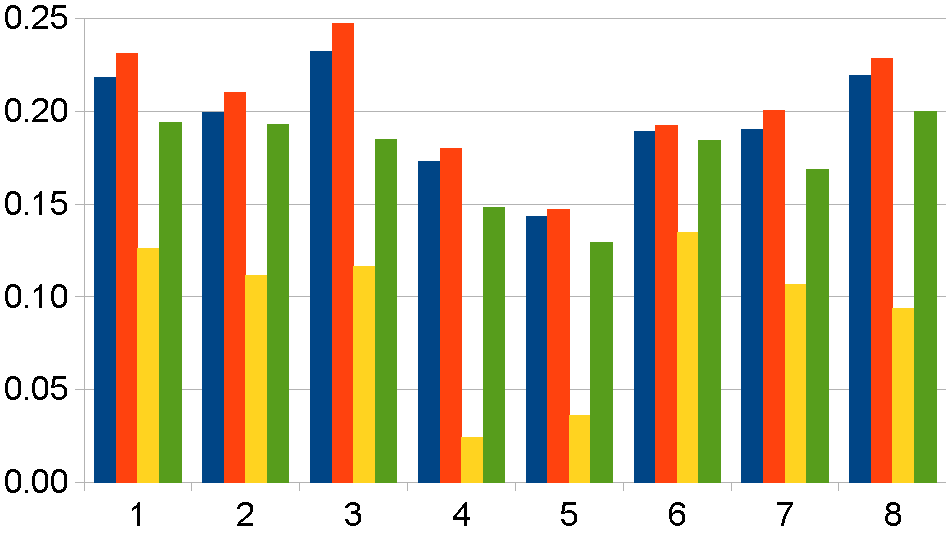
\includegraphics[page=1,width=0.9\textwidth]{graphics/tfm_results}};
        \node[below=of img, node distance=0cm, yshift=1cm,font=\color{black}] {TREC Track};
        \node[left=of img, node distance=0cm, rotate=90, anchor=center,yshift=-0.7cm,font=\color{black}] {Mean Average Precision};
    \end{tikzpicture}
    \begin{center}
        \begin{tabular}{ c c c c }
            \tikz\draw[dblue,fill=dblue] (0,0) rectangle (1.5ex, 1.5ex); No expansion
            \tikz\draw[dorange,fill=dorange] (0,0) rectangle (1.5ex, 1.5ex); Relevance feedback 
            \tikz\draw[yellow2,fill=yellow2] (0,0) rectangle (1.5ex, 1.5ex); QE
            \tikz\draw[green2,fill=green2] (0,0) rectangle (1.5ex, 1.5ex); tf-merging
        \end{tabular}
    \end{center}
    
\end{figure}

% \subsection{Hyponym Query Drift}
Let us inspect TREC-6 query 40, \textit{``land mine ban''}, to see what is really happening. With no query expansion, the AP (Average Precision) is 0.0805, with QE, the AP is 0.0014, and with tf-merging, the average precision is 0.0984. This query was chosen as QE clearly has a huge negative impact on this query, and tf-merging has a small positive effect. 

WordNet provides 180 hyponyms for the 3 query terms; 9 examples can be seen in Table \ref{example-query}. Some of these hyponyms like \textit{``ground emplaced mine''} appear relevant to the initial query. However, other terms like \textit{``goldmine''} are clearly irrelevant and could very easily cause query drift. Problematically, WordNet does not disambiguate polysemes and homographs, e.g.\ ``mine'' the explosive and ``mine'' the excavation site are conflated. More importantly, however, there are 153 expansions for the term ``land''. Hence, over 80\% of the modified query terms are either ``land'' or a hyponym of ``land'', this causes the query to drift towards land-ness, so documents exclusively about ``land'' are over boosted in the rank. Thirdly, many hyponyms for ``land'' are geographic labels and proper nouns, and proper nouns are known to cause query drift \cite{vechtomova2004use}.

%Using hypernym\textquotesingle s on Trec-6 query 14 improved from 0.0014 to 0.0102, a factor of 7.2 higher.
\begin{table}[h]
    \centering
    \small
    \begin{tabular}{|l|r|l l l|}
        \hline
        Query term & Expansions & \multicolumn{3}{c|}{Some example expansions} \\
        \hline
        \small
        land & 153 & crash land	& farmland 	& no man's land \\
        mine & 18  & goldmine		& booby trap 	& ground emplaced mine \\
        ban  & 9   & embargo		& rusticate 	& cease and desist \\
        \hline
    \end{tabular}
        \caption{Expansion hyponyms, TREC-6 query 40}
    \label{example-query}
\end{table}

With tf-merging, the query's retrieval performance was better than QE (and better than no expansion) as the excessive amount of ``land'' expansions did not cause query drift.

\subsection{Antonyms}
Our results showed that using antonyms as a source of expansion terms improves precision almost as often as synonyms. This initially seems counterintuitive as surely including the exact opposite of the query will retrieve the exact opposite results. However, this is not the case as antonyms can cause vocabulary mismatch just as synonyms can because you can describe something through its negation. The two sentences below are not strictly identical, but they convey a similar sense.

\begin{center}
    \textit{``I am \textbf{short}''}
    
    \textit{``I am \textbf{not tall}''}
\end{center}

Many antonyms are interdependent with their antonymous pair as each cannot exist without the other, e.g.\ the concept of \textit{``tallness''} depends on the concept of \textit{``shortness''}, as \textit{``shortness''} depends on the concept of \textit{``tallness''}. You cannot define one without defining the other. George Orwell also described this linguistic observation.

\begin{center}
    \textit{``what justification is there for a word which is simply the opposite of some other word? A word contains its opposite in itself. Take "good", for instance. If you have a word like "good", what need is there for a word like "bad"? "Ungood" will do just as well."}
    \\ --- George Orwell, 1984
\end{center}

Orwell's proposal to abolish antonyms was not sincere. It was part of \textit{newspeak}, a satirical spin on government censorship by means of \textit{reductio ad absurdum}.

Indeed, a common method to automatically find antonymous pairs is co-occurrence analysis \cite{JusteonKatz1991, justeson1991co}. The same method discussed previously that constructs statistical thesauri—the same method which finds synonymous pairs. According to the WordNet documentation, \textit{``direct antonyms''} are \textit{``a pair of words between which there is an associative bond resulting from their frequent co-occurrence''}, i.e.\ they have probably use co-occurrence analysis to identify antonyms.

% PROBLEM WITH WORDNET 
% Following a chain of antonmyms we arrive at a word which is unrelated to the first item in the chain,
% LEFT - RIGHT - WRONG - CORRECT

% Table \ref{tfmmap} shows the MAP of each TREC track using different query expansion techniques. The bold entries indicate an improvement over doing nothing. Rocchio's relevance feedback method shows that standard query expansion can consistently improve the mean average precision (MAP). However when using a general-purpose thesaurus (Roget/WordNet), standard query expansion degrades the MAP in all cases. These results are not unexpected. We can see that our tf-merging technique performs better than the standard approach, and occasionally performs better than doing nothing.

% %none v tf-merging	0.0027
% %none v query expansion	9.7804E-015
% %tf-mergingergin v query expansion	4.7525E-010

% \begin{table*}[t]
% \centering
% \caption{Mean Average Precision}
% \label{tfmmap}
% \begin{tabular}{|l|l|r|r|r|r|r|r|r|r|}

% \hline
% Expansion terms 				& mode	& TREC-1	& TREC-2	& TREC-3	& TREC-4	& TREC-5	& TREC-6	& TREC-7	& TREC-8 \\
% \hline
% No expansion				&				& 0.2181	& 0.1993	& 0.2324	& 0.1727	& 0.1432	& 0.1891	& 0.1905	& 0.2195 \\
% Relevance feedback				& naive		& \textbf{0.2311}	& \textbf{0.2103}	& \textbf{0.2476}	& \textbf{0.1802}	& \textbf{0.1468}	& \textbf{0.1925}	& \textbf{0.2007}	& \textbf{0.2286} \\
% \hline
% Roget				& naive		& 0.1995	& 0.1740	& 0.1945	& 0.1349	& 0.1119	& 0.1802	& 0.1853	& 0.2069 \\
% Antonym				& naive		& 0.1977	& 0.1823	& 0.2139	& 0.1411	& 0.1230	& 0.1618	& 0.1741	& 0.1977 \\
% Entailment			& naive		& 0.2153	& 0.1942	& 0.2315	& 0.1651	& 0.1311	& 0.1851	& 0.1898	& 0.2171 \\
% Hypernym			& naive		& 0.1220	& 0.0680	& 0.1139	& 0.0335	& 0.0475	& 0.1058	& 0.1011	& 0.1155 \\
% Hyponym			& naive		& 0.1258	& 0.1114	& 0.1161	& 0.0243	& 0.0362	& 0.1347	& 0.1068	& 0.0937 \\
% Meronym part		& naive		& 0.2154	& 0.1972	& 0.2250	& 0.1642	& 0.1402	& 0.1886	& 0.1896	& 0.2076 \\
% Meronym subs		& naive		& 0.2157	& 0.1839	& 0.2168	& 0.1593	& 0.1259	& 0.1860	& 0.1911	& 0.2095 \\
% Similar To			& naive		& 0.1760	& 0.1630	& 0.1754	& 0.1065	& 0.1074	& 0.1714	& 0.1715	& 0.2084 \\
% \hline
% Roget				& tf-m		& 0.2173	& 0.1986	& 0.2225	& 0.1609	& 0.1393	& 0.1877	& 0.1887	& 0.2041 \\
% Antonym				& tf-m		& 0.2157	& \textbf{0.2004}	& 0.2292	& 0.1718	& 0.1404	& 0.1851	& 0.1895	& 0.2161 \\
% Entailment			& tf-m		& 0.2180	& 0.1978	& 0.2324	& 0.1726	& 0.1319	& 0.1879	& 0.1900	& 0.2175 \\
% Hypernym			& tf-m		& 0.1446	& 0.1414	& 0.1553	& 0.1072	& 0.1012	& 0.1205	& 0.1104	& 0.1716 \\
% Hyponym				& tf-m		& 0.1940	& 0.1929	& 0.1846	& 0.1483	& 0.1292	& 0.1844	& 0.1686	& 0.1996 \\
% Meronym part		& tf-m		& \textbf{0.2190}	& \textbf{0.2022}	& 0.2307	& 0.1694	& 0.1406	& \textbf{0.1912}	& \textbf{0.1912}	& 0.2152 \\
% Meronym subs		& tf-m		& 0.2180	& 0.1993	& 0.2324	& 0.1727	& 0.1425	& 0.1891	& 0.1834	& 0.2195 \\
% Similar To			& tf-m		& 0.2075	& 0.1959	& 0.2183	& 0.1659	& 0.1301	& \textbf{0.1910}	& 0.1882	& 0.2041 \\
% \hline

% \end{tabular}
% \end{table*}




% \subsection{Speed}
% We did not focus our experiments on time efficiency but it's worth a quick mention. Relevance feedback is intrinsically slow as it require at least two passes through the search engine pipeline, and a complicated term selection process. On average, QE is about 10\% slower than no expansion, tf-mergning is about 20\% slower than no expansion, and relevance feedback is 317\% slower than no expansion. Although these results are clearly dependent on hardware and implementation which we can't guarantee are any good. Though we can say the speed differences are as expected.

%none 113.6575
%relevance feedback 324.38916666666665
%Qw 122.63833333333334
%QW 102.7425






%%%%%\section{Discussion}
%Using tf-merging may also reduce the impact of spurious terms, as their contribution is not considered 
%Since automatically selected expansion terms can be irrelevant to the original query, we reduce the effects of query drift. 

%%%%%If we could precompute the expansion terms for any given query, we could store these with the index and quickly recall them when required. Such a semantic mapping table would be \textit{almost} synonymous with a thesaurus, but not quite. An appropriate expansion term is not necessarily \textit{synonymous} with a query term, because a user generated query might not contain an important concept relevant to the information need. Users are usually unsure of the information they are requesting, which is why they are requesting it. This is why methods like blind relevance feedback are effective, because they find expansion terms which refer to concepts related to the users information need, but not contained within the initial query. 

%There are many content bearing terms that are not added to the query expansion. imprecise vocabulary.

% It may also inadvertently broaden the interpretation(s), leading to query drift, as we are not guaranteed that automatically selected expansion terms are relevant.
 %This is likely due to the fact that the vocabulary of the general-purpose thesauri we tested, do not coincide with the vocabulary of the corpus.
 %Perhaps with more adjustments a general-purpose thesaurus might be useful, but we must take the necessary precautions to prevent query drift, as they will unlikely reflect the vocabulary used in most documents collections. Specialized domain specific thesauri are recommended. 

%A thesaurus constructed specifically for a the document collection may provide better results. A corpus specific thesaurus could be done either manually, or through automatic means. Either way the vocabulary used in such a thesaurus would more likely coincide with the vocabulary of the corpus it was derived from. %










\section{Conclusions}

Our results agree with the literature. Query expansion is unreliable when using a semantic ontology (like WordNet or Roget) as a source of expansion terms. Even though WordNet 3.1 is more comprehensive, it is still not viable for na{\"i}ve query expansion. This is because WordNet is a lexical-semantic ontology that cannot disambiguate polysemous and homographic words, which leads to poor quality expansion terms, resulting in query drift.

% Relevance Feedback, which is statistical in nature and collection dependent is more reliable.
% We could also blame the fact that it's a global, collection independent source of expansion terms. 

Hyponyms (and hypernyms) are ineffective for expansion. Antonyms are surprisingly effective because they have similar linguistic properties to synonyms.

Term Frequency Merging can be implemented at index time. This would require the indexer to identify synonyms (or SynSets) across the document collection and replace them with the same term (lexical token). The benefit to this approach would be the zero cost to merge at search time. However, disambiguating polysemes and homographs would still pose an an issue.

Many other expansion models could easily implement tf-merging but unfortunately not Relevance Feedback, since its expansion terms derive from documents, not directly from individual query terms, so it is not immediately clear which expansion term should be merged with which original query term.

If the expansion terms are of poor quality, tf-merging does little to help. Our method only improves retrieval in the particular case where there is query drift caused by an uneven distribution of expansion terms, i.e.\ one query term has more expansions than another.


% The purpose of our experiments was to determine if using general-purpose thesauri for query expansion could be improved. We tested two different thesauri (Roget and Wordnet), with two different query expansion techniques. We compared standard query expansion with our proposed method that we call tf-merging.

% Our results agree with the literature, using a general-purpose thesauri appears to have potential but lacks reliability. Despite the fact that WordNet has become more comprehensive as a thesaurus, it is still not viable for QE. It \textit{can}, and frequently does, improve the precision of ad-hoc retrieval tasks, but there is still a large chance that the precision will be degraded. 

% Reformulating a query through tf-merging makes sense intuitively, as we are not biasing our search towards query terms which have more expansions. What we have proposed is straightforward and efficient, and it does not require a sophisticated language model to be implemented. Our approach of tf-merging does empirically improve general-purpose thesauri query expansion, but not enough to be competitive against other query reformulation methods.

% compare to other people's work
% Since our results indicate an improvement to thesaurus based expansion, in future work we will apply tf-merging to other query reformulation methods. The most obvious choice would be relevance feedback approaches, as their effectiveness is well established, especially the RM3 relevance model \cite{abdul2004umass}. Since tf-merging is independent of the expansion term selection process, it could easily be used to complement existing query expansion improvements. We will also test the effectiveness with other ranking functions that use TF and IDF scores.



% It is likely that tf-merging will fail to reduce the effects of query drift, when there are many discriminating spurious terms in every expansion set. But if the expansion term selection process is good, then tf-merging should be able to improve it.

% We suspect that tf-merging can reduce the negative effects of query drift, when the spurious terms are far less common than the favorable expansion terms. If the expansion term selection process is dreadful, then tf-merging will struggle to improve it by very much.


% \section{Statistics}
% Statistics
% two standard deviations from the mean
% outside the range
% but still perfectly normal
% performing the experiment 20 times, one outside the range
% this would be as expected
% now the results so far, are definitely outside the expected range
% that doesn't definitively conclude that the results have improved, or even changed, the difference could still be random noise
% but it some evidence that there is a degree of bias towards improvement
% Again, the bias isn't confirmed, unequivocally
% but it's just a failure to reject
% There is undeniable plausibility
% If I were a betting man, I would bet money on this (not too much mind you, I'm a broke Masters student)
% There is no way to confirm the results of this experiment, or increase the p value to ??? ... 100%
% Instead of inferring whether or not a user has succeeded in full-filling the information request by analysing their behaviour

        \chapter{Query Context Selection}

% better name
% L  Local 
% QC Query Context 
% ET Expansion Term
% R  Refinement
% S  Selection

%\section{Natural Disambiguation}

% And not just the literal semantics of the words, but also the delivery, and inflection, the context of the occurrence of the statement, the social context, the political context, 

% Natural effortless disambiguation

Is it possible to have a context-free word? As my Dad always says:

\begin{center}
    \centering
    \textit{``Yes''}
\end{center}

The human mind can disambiguate the meaning of individual words by accounting for the wider context. For example, in the Oxford English Dictionary, \textit{``set''} has over 430 definitions making it the most polysemous word in the English language. However, within the context of the sentence \textit{``we must set out before dawn''} it does not seem ambiguous to me. A fluent reader can naturally disambiguate with amazing cognitive ease through the semantics of the other words and the surrounding grammar. You are doing it now; look at you go!

Here is an easier example to explain. In the following four sentences, can you assign a single word sense to each occurrence of \textit{``bank''}?

\begin{enumerate}
    \item \textit{``It's a \textbf{bank}.''}
    \item \textit{``They made all of their profits from the rushes on the \textbf{banks}''}
    \item \textit{``I saw three bears by the river \textbf{bank}.''}
    \item \textit{``I was \textbf{banking}\textsubscript{1} on the aeroplane to \textbf{bank}\textsubscript{2} into the river \textbf{bank}\textsubscript{3}, for I had over insured it with my \textbf{bank}\textsubscript{4}''}
\end{enumerate}

The first is impossible as the context is too vague. The second is impossible as it is a cleverly contrived pun. Number three is just right. The fourth sentence is an antanaclasis and contains 4 occurrences of the word ``bank''. Each can be disambiguated by considering the words preceding and following the term of interest. For example, \textit{bank}\textsubscript{3} is preceded by the attributive noun \textit{river}, which is preceded by the determiner \textit{the}. So the word sense of \textit{bank}\textsubscript{3} is clearly the land alongside a river. Table \ref{bank-definitions} shows all four intended definitions in the antanaclasis.

% Restricted expansion of query terms using part of speech tagging
% https://patents.google.com/patent/US5721902A/en

\begin{table}[h]
\centering
\begin{tabular}{|l|l|l|}
\hline
Term    & Part of speech & Definition                          \\ \hline
\textbf{\textit{bank on}}\textsubscript{1} & phrasal verb & To rely on confidently.             \\
\textbf{\textit{bank}}\textsubscript{2}    & noun & The land alongside a river or lake. \\
\textbf{\textit{bank}}\textsubscript{3}    & verb & To tilt sideways in making a turn.  \\
\textbf{\textit{bank}}\textsubscript{4}    & noun & A financial establishment.          \\ \hline
\end{tabular}
\caption{Four (of 18) Possible Definitions of the Term \textit{bank}}
\label{bank-definitions}
\end{table}

% It should be clear that polysemes (and homographs) can be naturally disambiguated using the other words in the sentence.

\section{Na{\"i}ve Expansion Selection} \label{standardTS}
The na{\"i}ve approach to query expansion with a semantic ontology is to include \textit{\textbf{all}} the provided candidate expansions without restriction. This is problematic since it is unlikely that a single query term refers to more than a single word sense. This problem becomes apparent when considering polysemes (and homographs). For example, if one were expanding the query term \textit{``bank''} with a thesaurus, it would make no sense to select \textit{``embankment''}, \textit{``tilt''} and \textit{``treasury''} as expansions since the author likely intended only one distinct word sense, not three.

Selecting every candidate expansion does increase the chance of selecting the right one, but it also vastly increases the chance of selecting many more incorrect ones. If spurious terms are chosen for expansion, the modified query will experience drift towards various unrelated concepts. 




\section{Better Expansion Selection} \label{betterTS}
A better approach would be to disambiguate the word sense of the ambiguous terms and only include expansion terms which share the same word sense. Though, if we did have an immediate method to determine word sense, we would not be attempting to find a solution with a thesaurus.

Selecting expansion terms from a single thesaurus entry would be a good approach if we had a method to determine which word sense the query author \textit{most likely} intended. Let us first suppose that all (or most) of the original query terms relate to the same concept, i.e.\ the user's information need. Unfortunately, query intent is not something that exists in WordNet; however, the query's SynSets may overlap semantically with the information need. 

% have some semantic association which can be discovered through the structural links in WordNet.

A possible solution is for every original query term, retrieve all of the associated SynSets. If there is only one associated SynSet, then select all the terms in that SynSet. If there is more than one associated SynSet, select the SynSet which is \textit{most similar} to the other query terms' SynSet(s). Where we define similarity as a function of traversal distance in the WordNet graph. More specifically, we will perform a pair-wise similarity comparison tournament between the SynSets, selecting the most similar SynSet and ignoring the less similar, and likely spurious SynSet(s) that would cause query drift.


% Discriminating ideal expansion terms from spurious ones is achieved by inferring their relevancy to the original query's context. 

% To reduce impact of \textit{query drift} by refining the set of candidate expansion terms.

% using the \textit{query context} to inform the expansion term selection process. Using WordNet as an initial source of expansion terms, we refine the candidate expansions by discriminating relevancy. We found that our term selection process is more effective than the standard approach. Our technique targets terms which relate to the entire query as a whole, but predominately focuses on excluding spurious expansion terms. Both help reduce query drift and increase query performance.

% \begin{figure}[h]
% \centering
% 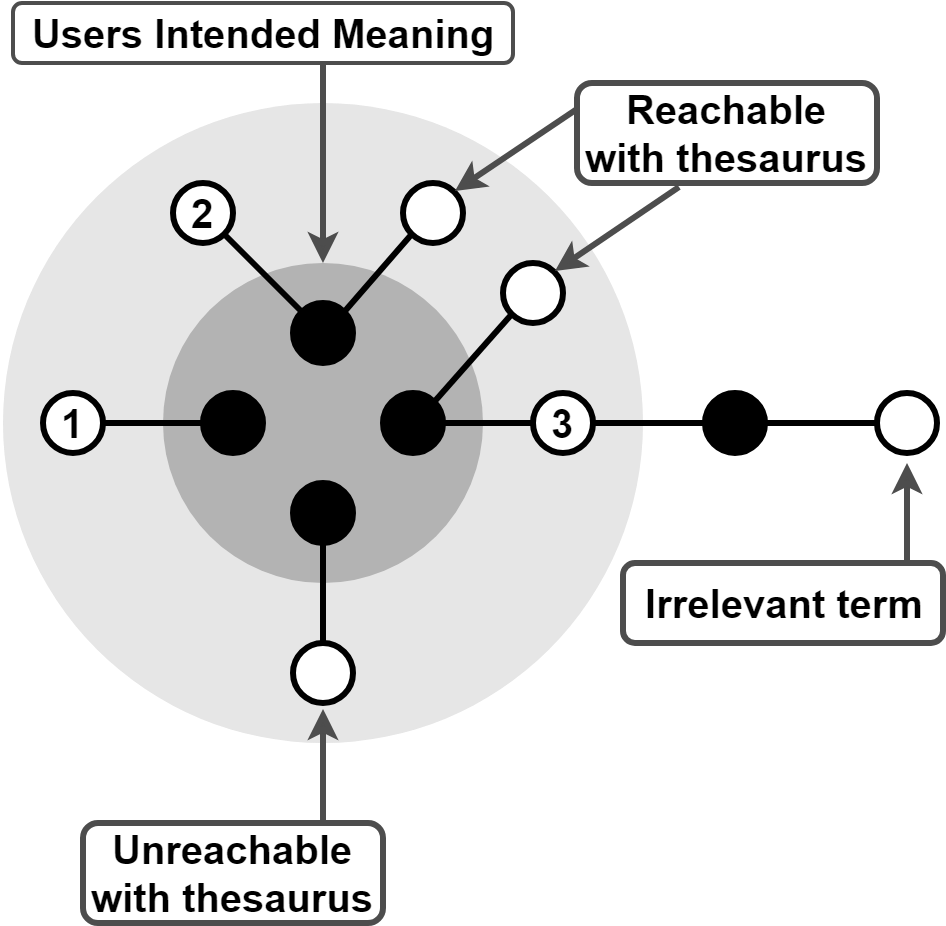
\includegraphics[width=0.6\linewidth]{graphics/query_semantic_space_labels.png}
% \caption{Query terms: 1, 2 and 3. Their SynSets (black circles) in a shared space.}
% \label{fig:querydiagram}
% \end{figure}

\begin{figure}
    \centering
    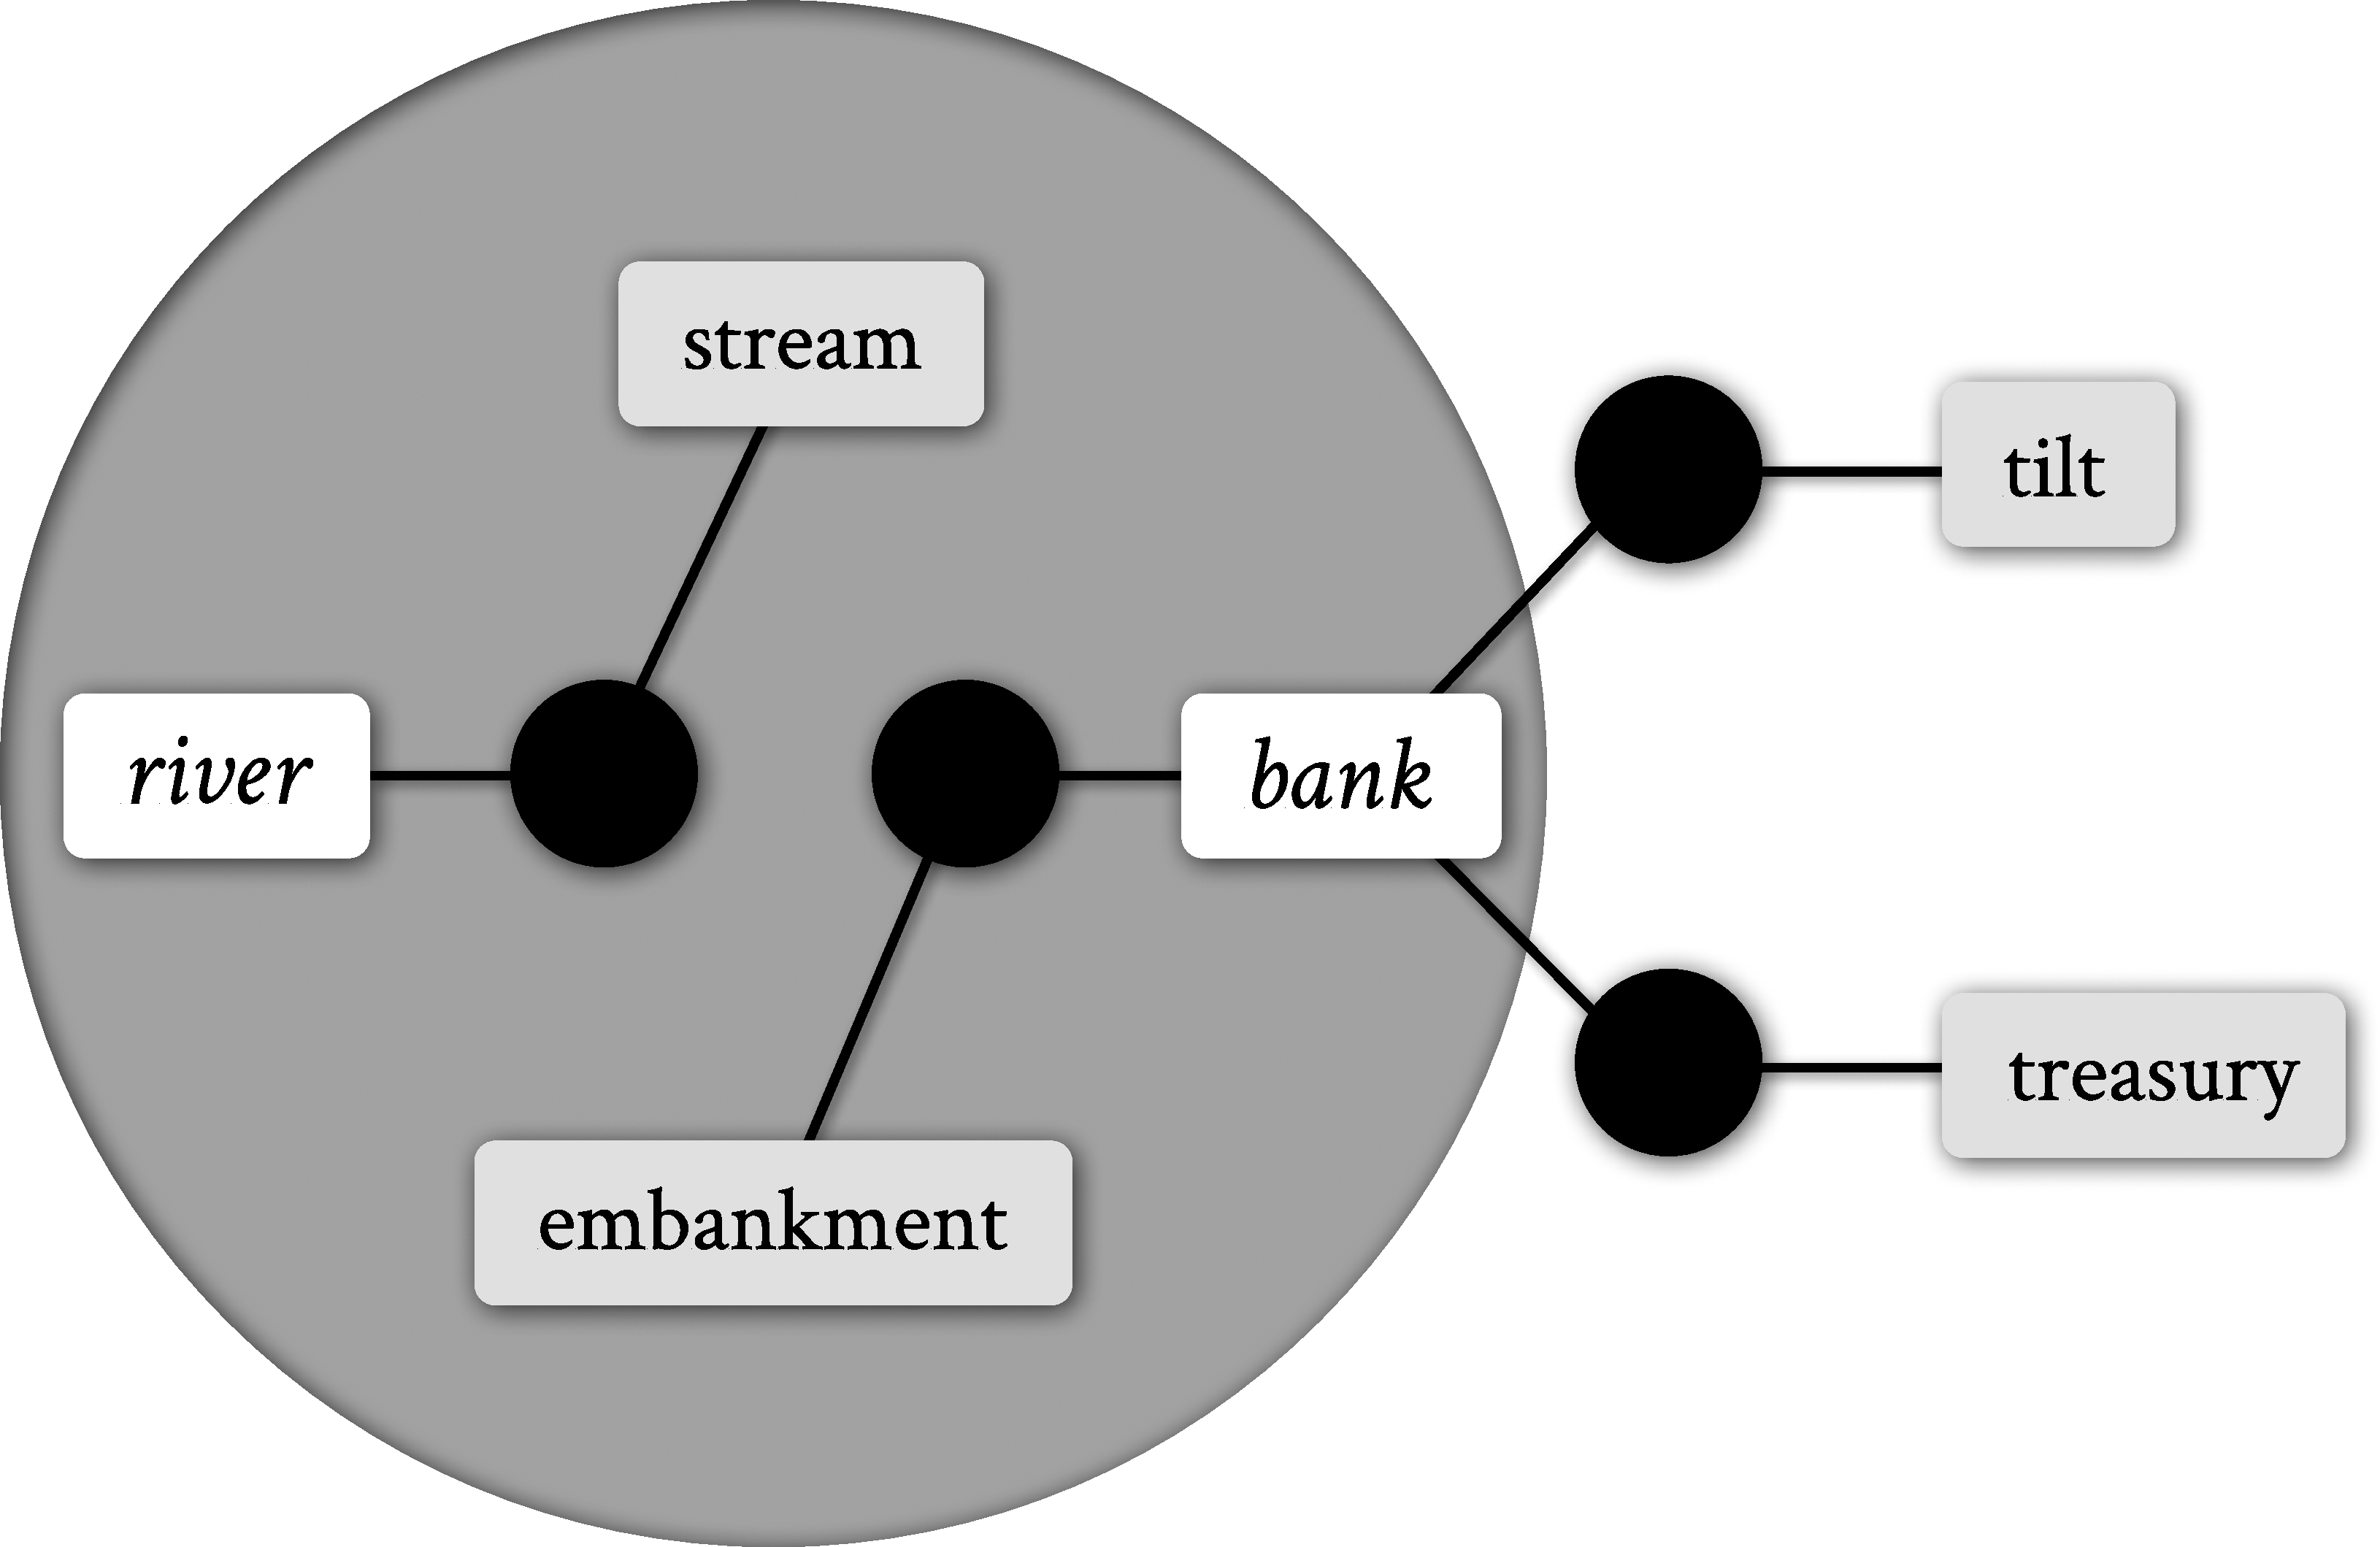
\includegraphics[width=0.7\linewidth]{graphics/concept-space.pdf}
    \caption{Concept space for query terms $Q = \{river, bank\}$ and potential expansion terms $E_Q = \{stream, embankment, tilt, treasury\}$. Black circles are SynSets with edges representing term membership. The grey circle represents the shared concept space, the user's intended meaning.}
    \label{fig:conceptspace}
\end{figure}

Figure \ref{fig:conceptspace} is an example query $Q = \{river, bank\}$, showing the relationship between the query terms, expansion terms, and SynSets, similar to Figure \ref{fig:sense-relations}. The terms and SynSets are superimposed into a conceptual space representing the user's intended meaning, their information need. The query term ``river'' is not polysemous, it's a member of one SynSet. However, bank is a member of 3 SynSets, two of which are located outside the concept space which would lead to query drift if included in the expanded query. No tournament would be necessary for ``river'', however ``bank'' requires a tournament to find the best SynSet for expansion, ideally the one which has ``embankment'' as a member.

% Figure \ref{fig:querydiagram} is an example query showing the relationship between terms (lexical tokens) and SynSets (word sense) similar to Figure \ref{fig:sense-relations}. The terms and SynSets are superimposed into the conceptual space of the information need; the user's intended meaning. The original query terms are identified with the white circles: 1, 2 and 3; the SynSets are black circles, with edges between showing WordNet (or other ontology) associations. The containing grey circle(s) represent the user's information need. Term 1 is a monoseme and has one associated SynSet. Term 3 is polysemous, as there are 2 SynSets; one contained within the information need and the other outside the information need, which is spurious and would cause query drift.

% Figure \ref{fig:querydiagram2} shows the proposed tournament resulting from the query \textit{``river bank"}. We can see that \textit{``river''} has 1 SynSet, so no tournament necessary. However, \textit{``bank''} has 3 SynSets, so we must determine which is the best for expansion. Clearly, the SynSets containing \textit{``tilt''} and \textit{``treasury''} are spurious for this query and the SynSet containing \textit{``embankment''} is not spurious.

% We choose a single SynSet by comparing the candidate expansion terms to the query context, i.e.\ the other SynSets. From a pairwise tournament the highest scoring SynSet is chosen as source for expansion terms.

% \begin{figure}
%     \centering
%     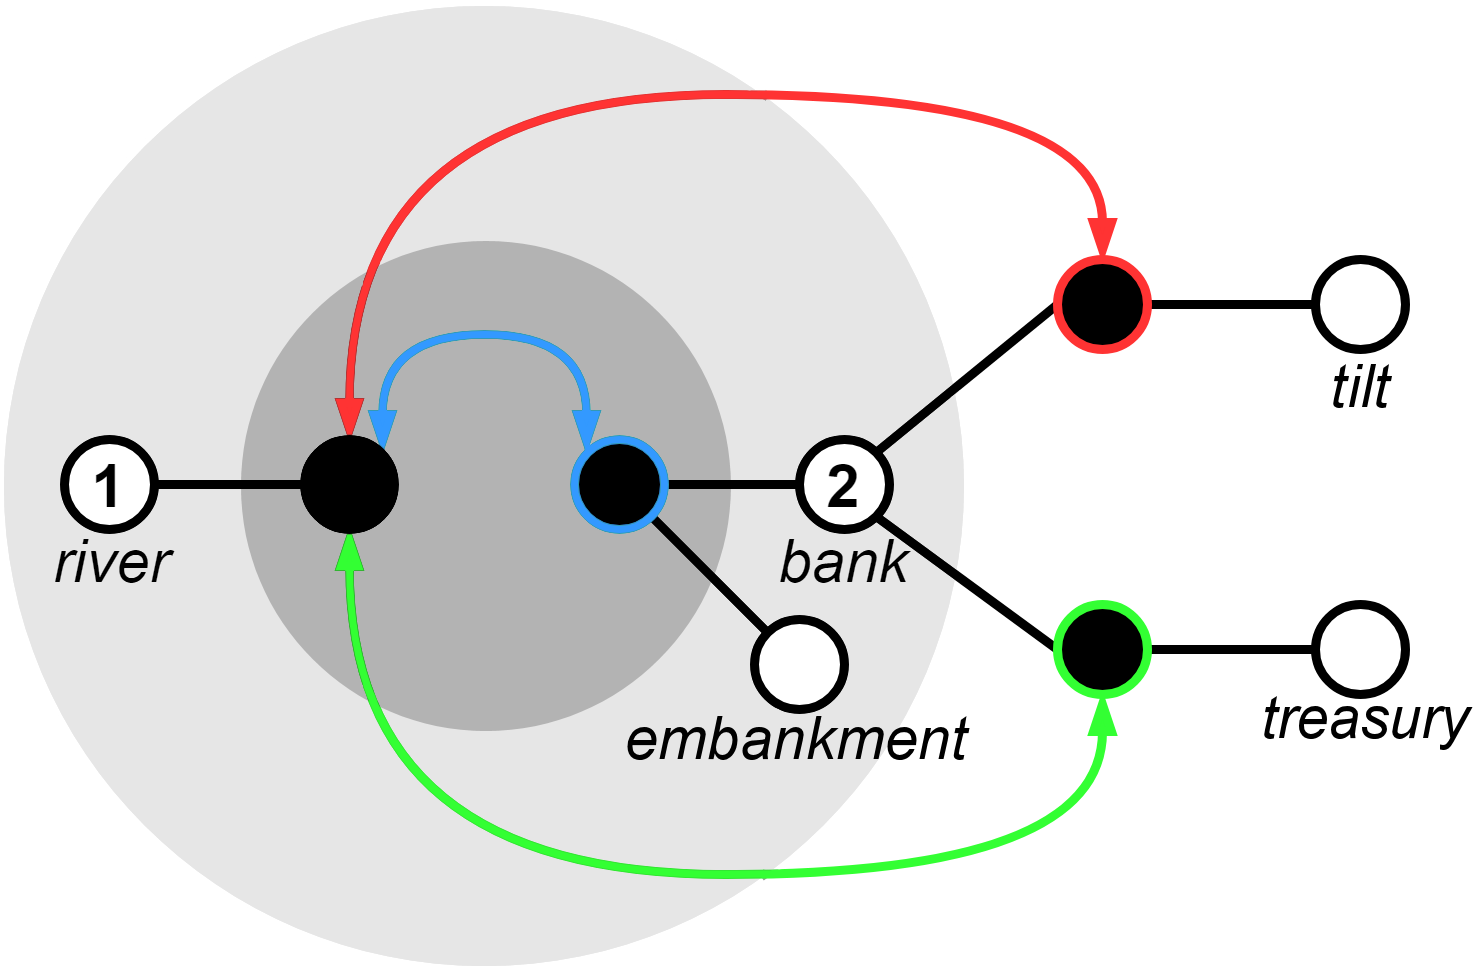
\includegraphics[width=0.6\linewidth]{graphics/tournament-2.png}
%     \caption{Tournament for the query \textit{``river bank''}}
%     \label{fig:querydiagram2}
% \end{figure}

\subsection{WordNet Structure}
We now take a closer look at the ontological structure of WordNet \cite{Miller:1995:WLD:219717.219748}.

\vspace{5pt}

\noindent \textbf{SynSet} Synonym set. A set of words that share at least one word sense, i.e.\ a single thesaurus entry.

\vspace{5pt}

\noindent \textbf{SynSets} Set of all word senses for a given term, i.e.\ potential candidates for the authors intended meaning(s). 

\vspace{5pt}

\noindent \textbf{Lemmas} Set of lexically distinct but \textit{``synonymous''} terms belonging to a SynSet.

\vspace{5pt}

% \vspace{\baselineskip}

% \noindent\textbf{Term}
% A string of characters. Can exist independent of meaning.
% \noindent\textbf{Word}
% A term authored with intended meaning, which is dependent on the context in which it was written. In rare cases, multiple meanings are simultaneously intended e.g.\ double entendre.
% \noindent\textbf{Word Sense}
% A well defined meaning associated with a term.
% \noindent\textbf{Synonyms}
% Terms that share same Word Sense.
%\noindent\textbf{Lexeme} Set of terms that share same Word Sense AND stem (e.g.\ different tenses)
%\noindent\textbf{Lemma} Canonical form or root term of a Lexeme.

\begin{figure}
    \centering
    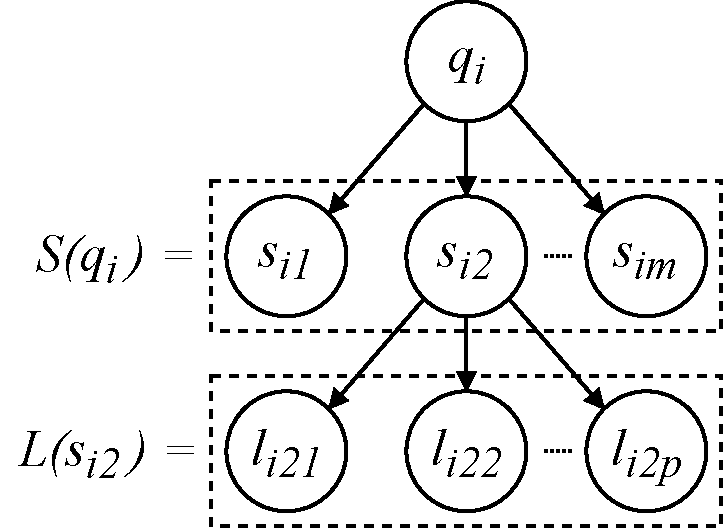
\includegraphics[width=0.6\linewidth]{graphics/lemma_diagram.pdf} 
    \caption{WordNet SynSets: ($q_i$) is the initial term; $S(q_i)$ are it's SynSets, and $L(s_{ij})$ are the lexical terms contained in each SynSet.}
    \label{fig:wn}
\end{figure}

\noindent
Figure \ref{fig:wn} shows how a query term ($q_i$) associates to many SynSets ($S(q_i)$), and subsequently many more lemma terms ($L(S(q_i))$), which are used as expansion terms. If the SynSet is a reflexive relation, then one of the lemma terms ($l_{ij}$) will be lexically identical to the initial query term ($q_i$).


\subsection{The Comparison Function}
As discussed earlier, in IR, it is common to compute term similarity using the corpus statistics, e.g.\ the dice coefficient, Jaccard Index and point-wise mutual information \cite{Carpineto:2012:SAQ:2071389.2071390}. They all infer similarity from co-occurrence data, a form of \textit{syntactic similarity}. We will instead measure \textit{semantic similarity} using the structural relationships in WordNet. We will measure the similarity between SynSets by measuring the path from one SynSet to another SynSet. The supposition is that path length correlates with semantic similarity, longer paths indicate lower similarity, and shorter paths indicate higher similarity. This is clearly true for neighbours, where path length equals 1, meaning the terms share a SynSet. We will use the Wu-Palmer function \cite{Wu:1994:VSL:981732.981751}, formally defined in Equation \ref{eq:d}, to find the shortest path. Wu-Palmer also accounts for large conceptual leaps by considering the lowest common subsumer (first shared ancestor) and weighting edges according to their depth within the hierarchy such that edges between more conceptual nodes (which are closer to the root) have a higher cost. 

% Since Word Senses which are separated by a shorter path are generally more semantically similar than those with a longer path.

\begin{figure}
    \begin{flalign}
        & & distance(a, b) & = \frac{2 * depth(LCS(a, b))}{depth(a) * depth(b)} & \label{eq:d} \\
        & & LCS(a, b) & = \text{Least Common Subsumer} & \label{eq:e} \\
        & & depth(a)  & = \text{Shortest path from root to } a & \label{eq:f}
    \end{flalign}
    \caption{Wu-Palmer distance function.}
\end{figure}

% \begin{flalign}
% &  & Q  & = \{ q_1, q_2, ... q_n \} &  & \text{Query terms}\label{eq:a} \\
% &  & S(q_i)  & = \{ s_{i1}, s_{i2}, ... s_{im} \} &  &  \text{Synonym set}\label{eq:b}\\
% &  & L(s_{ij}) & = \{ l_{ij1}, l_{ij2}, ... l_{ijp} \} &  &  \text{Lemma terms}\label{eq:c}
% \end{flalign}

% $ sim(a,b) = frac{2 * depth(LCS(a, b))}{depth(a) * depth(b)} $
% sim(a, b)  similarity
% depth(a) = shortest path from root to a
% lcs(a, b) = lowest common subsumer of a and b, (closest shared ancestor).

% We will refer to the term being expanded as the \textit{term of interest}, and the set of remaining terms from the original query as the \textit{other terms}. 

\subsection{The Tournament}
The SynSets for each query term will be compared to the SynSets of the other terms using Wu-Palmer distance as the comparison function. The highest scoring SynSet wins the tournament and is chosen as the most likely candidate for the intended word sense. Then each of the lemma terms from the winning SynSet are added to the modified query. This process is repeated for each term in the original query. The algorithmic complexity of this process is exponential with respect to the number of query terms and the number of associated SynSets. However, in practice, the performance is reasonable since queries are short and the number of SynSets is usually quite small (except in rare cases like \textit{``set''}).

\subsubsection{A Successful Example}
%\begin{displayquote}
For the query $Q_1 = \{``river '', ``bank''\}$, \textit{``river''} has only 1 SynSet, and \textit{``bank''} has 18. Therfore, only 18 comparisons need to be made. Our method correctly identifies the SynSets:

\vspace{5pt}

\noindent
\textbf{river} \textit{``a large natural stream of water (larger than a creek)''} 

\vspace{5pt}

\noindent
\textbf{bank} \textit{``sloping land (especially the slope beside a body of water)''}

\vspace{5pt}

\noindent
This suggests that the Wu-Palmer distance function is capable for our use case.

% Supposition is that the query terms correlate e.g. ball -> pool cue -> pool
% Disamguiate ball from beach ball, or formal dance


% re explain the experiment ? ATIRE TREC...

\subsubsection{An Unsuccessful Example}

\noindent For the query $Q_2 = \{``pool '', ``cue''\}$, \textit{``pool''} has 11 SynSets, and \textit{``cue''} has 5. Therefore, 55 comparisons need to be made. The SynSets identified by our method are:

\vspace{5pt}

\noindent
\textbf{pool} \textit{``an excavation that is (usually) filled with water''}

\vspace{5pt}

\noindent
\textbf{cue} \textit{``sports implement consisting of a tapering rod used to strike a cue ball in pool or billiards.''}
% \vspace{\baselineskip}

\vspace{5pt}

\noindent
Our method failed for \textit{``pool''}, suggesting this method is not perfect in every case.

\section{Results}
% Parameters chosen Top 17 documents, top 5 terms.
Table \ref{table:results} shows our results on the TREC ad-hoc retrieval tracks. Included for comparison is a baseline (\textit{None}), which is no expansion, and the benchmark blind relevance feedback (\textit{RF}). Bold entries indicate the best result for the track. The main results from our experiments are labelled \textit{All-SynSets} (the standard approach described in section \ref{standardTS}), and \textit{One-SynSet} (our improved method described in section \ref{betterTS}). We also included two separate query reformulation techniques. The na{\"i}ve approach of appending terms directly to the query and term-frequency-merging (\textit{tfm}) \cite{Crimp:2017:ATR:3166072.3166074} described in Chapter \ref{chap:tfm}. Term-frequency merging attempts to reduce query drift caused by uneven numbers of expansion terms, which should be less of a problem for the \textit{One-SynSet} case.

The results are promising, as can be seen in Table \ref{table:results}. The standard approach \textit{All-SynSets} with \textit{na{\"i}ve QE} only beats the baseline in one case (TREC-6). In comparison, our method \textit{One-SynSet} with \textit{na{\"i}ve QE} improves upon the baseline in all but one case (TREC-6). And \textit{One-SynSet} with \textit{tf-merging} beats the baseline in all cases. Blind relevance feedback is still a strong contender as it remains unbeaten in TREC-1, TREC-2 and TREC-3.

%This is clear from the results, as \textit{All SynSets} was the best choice in TREC-5, TREC-6 and TREC-8. Even though this method includes many spurious terms, it's guaranteed to include a few relevant terms.

We calculated two-tailed $t$-tests on the 400 paired MAP samples. Comparing the baseline against, All-Synsets, and One-SynSet, and in every case, we obtained $p$-values $< 0.05$, which suggests that the observed differences cannot be attributed to chance alone.

% none vs onesynset_lemma = 0.01128541
% none vs all_synset_head_word = 0.5462267


%For each query term, we take every possible Word Sense, and for every possible 

%two terms to distinguish the two different modes, for expansion term selection

%1) All SynSets 
%2) One SynSet

%restricted term selection using information from the query context

%query context informs expansion term selection




\begin{table*}[h]
\centering
\resizebox{\textwidth}{!}{
\begin{tabular}{|l|l|r|r|r|r|r|r|r|r|}
\hline
Term Selection  & Expansion     & TREC-1          & TREC-2          & TREC-3          & TREC-4          & TREC-5          & TREC-6          & TREC-7          & TREC-8          \\ \hline \hline
None            & N/A              & 0.2181          & 0.1993          & 0.2324          & 0.1727          & 0.1432          & 0.1891          & 0.1905          & 0.2195          \\
RF              & na{\"i}ve QE         & \textbf{0.2601} & \textbf{0.2521} & \textbf{0.2988} & 0.2041          & 0.1369          & 0.1646          & 0.2185          & 0.2460          \\ \hline
All-SynSets       & na{\"i}ve QE     & 0.2128          & 0.1961          & 0.2243          & 0.1265          & 0.1327          & 0.2041          & 0.1822          & 0.2187          \\
One-SynSet               & na{\"i}ve QE     & 0.2318          & 0.2104          & 0.2398          & 0.2101          & 0.1476          & 0.1781          & 0.2163          & 0.2301          \\ \hline
All-SynSets       & tfm           & 0.2323          & 0.2095          & 0.2379          & 0.1721          & \textbf{0.1618} & \textbf{0.2214} & 0.1953          & \textbf{0.2440} \\ 
One-SynSet               & tfm           & 0.2380          & 0.2286          & 0.2529          & \textbf{0.2179} & 0.1537          & 0.2007          & \textbf{0.2211} & 0.2310          \\ \hline
\end{tabular}
}
% \caption{Mean Average Precision Across TREC 1-8}
\caption{Comparing the MAP of our (One-SynSet) method to the standard (All-SynSets) method. With no expansion (None) as a baseline and relevance feedback (RF) as a benchmark. Across 8 TREC tracks, bold entries are the top result. $t$-tests between each of the 400 paired MAP samples produced $p$-values $< 0.05$.}
\label{table:results}
\end{table*}


\subsection{Failure Analysis}

%Including expansion terms from all SynSets does improve query performance x percent of the time. 

%Which suggests that the centroid of the query is 
If we look at the results for TREC-7 query 2: \textit{``british chunnel impact''} in Table \ref{table:T-7-2-map}, we can see that our method has an enormously positive impact. This is partly because it only includes 8 extra terms from 3 SynSets (one for each term), instead of the na{\"i}ve All-Synset approach, which includes 21 terms from 9 different SynSets causing significant query drift. More specifically, the lemma terms from \textit{impact} include \textit{``touch, bear, shock''}, which causes significant query drift in the All-SynSet case.

\begin{table}[h]
\centering
\begin{tabular}{|l|l|l|}
\hline
Term selection  & Expansion  & AP      \\ \hline
None (baseline) &            & 0.0513 \\
All-SynSets     & appending  & 0.0421 \\
All-SynSets     & tf-merging & 0.0509 \\
One-SynSet      & appending  & 0.3118 \\
One-SynSet      & tf-merging & 0.2045 \\ \hline
\end{tabular}
\caption{TREC-7 query 2 Average Precision}
\label{table:T-7-2-map}
\end{table}

%\begin{table}[h]
%\centering
%\caption{TREC-7 query 2 Expansion Terms for \textit{``impact''}}
%\label{table:T-7-2-expansions}
%\begin{tabular}{|l|llll|}
%\hline
%All-SynSets & impact & affect       & bear        & upon \\ \hline
%One-SynSet  & impact & encroachment & impengement &      \\ \hline
%\end{tabular}
%\end{table}

However, if we look at TREC-7 query 15 in Table \ref{table:T-7-15-map}, \textit{``el nino''}, our method is ineffective. Inspecting the expansion terms chosen, shown in Table \ref{table:T-7-15-expansions}, we can see that the term \textit{``el''} is incorrectly identified as the \textit{Chicago ``L'' Train}. This example is particularly bad as \textit{``el nino''} is a recent loan word from Spanish which does not yet exist in WordNet.

\begin{table}[h]
\centering
\begin{tabular}{|l|l|l|}
\hline
Term selection  & Expansion  & AP      \\ \hline
None (baseline) &            & 0.7861 \\
All-SynSets     & appending  & 0.7843 \\
All-SynSets     & tf-merging & 0.8466 \\
One-SynSet      & appending  & 0.1947 \\
One-SynSet      & tf-merging & 0.8120 \\ \hline
\end{tabular}
\caption{TREC-7 query 15 Average Precision}
\label{table:T-7-15-map}
\end{table}

\begin{table}[h]
\centering
\begin{tabular}{|l|lllll|}
\hline
All-SynSets & alt & altitude & el       & elevation & ...        \\ \hline
One-SynSet  & el  & elevated & railroad  & railway & ... \\ \hline
\end{tabular}
\caption{Some expansion for the query term \textit{``el''}, in TREC-7 query 15}
\label{table:T-7-15-expansions}
\end{table}

% \subsection{Using the Similarity Score as a Predictor}
% The larger the similarity score, the more relevant the SynSet is assumed to be. So it is obvious to try and use the similarity score to predict the improvement of the modified query. Measuring the correlation using the Pearson bivariate method gives a score of approximately 0 ( precisely $-0.0617$ ). This suggests \textit{no} simple correlation between the \textit{Wu-Palmer Similarity Score} and the \textit{Mean Average Precision improvement (from the baseline)}. 

%It seems the score is tightly linked to the terms it is computed from. Because even a winning score from a tournament can be relatively small (compared to other tournaments) and yet, it can still improve the query. And occasionally a really large score will fail to improve a query, by misidentifying the intended Word Sense.

\section{Future Work}
Our method is essentially performing word sense disambiguation on polysemes where SynSets are treated as \textit{word sense}. There is still no assurance that our method correctly identifies the intended word sense of the original query term(s) as it is limited by the semantics of the query context. It still ignores many other features like syntactic grammar.

Our current method could, for example, select a noun-SynSet for a query term that is grammatically a verb. WordNet provides \textit{part of speech} tagging by indicating which lexical category the SynSet belongs to (e.g.\ noun, verb, adjective, etc.). Accounting for the lexical category could improve our results, but it would require the queries to be written with correct syntactic grammar, which is not guaranteed.

% \cite{Voorhees:1994:QEU:188490.188508}

The Wu-Palmer distance function is a pair-wise comparison and is ideal for queries with only 2 terms. For longer queries, a tournament of comparisons is needed, but performing a group-wise comparison directly would be more appropriate, like the group-wise Jaccard Index or the group-wise Resnik comparison \cite{Manda327833}. Comparisons of SynSets within WordNet is based on finding the shortest path in the graph. A group-wise comparison would be equivalent to finding the minimal subgraph that includes at least one SynSet from each query term. This subgraph would be a tree since a minimal graph has no cycles. The tree's intermediary nodes (SynSets) used to construct the tree could also be used for expansion terms. This can be described as a variant of the Prize Collecting Steiner tree problem \cite{Johnson:2000:PCS:338219.338637}, where we would minimize edge cost and maximize vertex profit. 

% In our case, profit would be indicated by \textit{stop words} having small values and \textit{content bearing terms} having high values. This is an NP-hard problem.

\section{Conclusions}
Overall, our results are promising. Blind relevance feedback remains a strong option as it can find expansion terms that are not semantically related to any of the original query terms, i.e.\ it can include related concept(s) that the user did not think to include, which is beyond the scope of vocabulary mismatch.

Using our query context informed method, we refined the expansion terms obtained from a thesaurus, which is more effective than using a thesaurus blindly. Term frequency merging was able to be applied to both methods and improved them in all cases. 

% We assumed that WordNet is sufficiently complete

% We also assumed that lemma terms would exist at the same level




    
    \part{Discussions}
        \chapter{Experimental Limitations}

% \begin{flushright}
% \textit{``Behind it all is surely an idea so simple, so beautiful, that when ---in a decade, a century, or a millennium--- we grasp it, we will all say to each other, how could it have been otherwise? How could we have been so stupid for so long?''}
% \\ --- John Archibald Wheeler
% \end{flushright}




I began this thesis with great hubris. I was investigating something I knew nothing about, but now that I am almost done, after years of research, long nights spent reading at the library and typing behind a computer screen, I have finally reached the point where I can say, with absolute certainty, beyond all reasonable doubt, that I \textit{definitely} know nothing.

\section{The Limitations of Evaluation Data}
An unaddressed issue is the assumption that the evaluation data is sound and complete, i.e.\ the source of ground truth is true and that its coverage is comprehensive. Which is not easy to prove, as there are hundreds of thousands of documents in these test collections, over a million (1,367,000) in the ones I used. If the qrels are incomplete, if a relevant document exists in the collection that is not present in the qrels, then retrieving this previously unidentified document could negatively impact the accuracy metrics.

Another unaddressed issue is the presence of inconsistencies in evaluation data sets. As described previously, Vocabulary Mismatch is pervasive. Even experts use inconsistent vocabulary when describing the same concept. Similarly, experts are inconsistent when constructing evaluation data \cite{schamber1994relevance}. Relevance judgements can differ for each judge and for the same judge at different times. This is because the evaluation data is constructed from language, we all use language differently, and we all read language differently. We each have our own personal view on language. This is called an idiolect; it is the dialect specific to a person.

%%%%%%%%%%%%%%%%%%%%%%%%%%%%%%%%%%%%%%%%%%%%%%%%%%%%%%%%%%%%%%%%%%%%%%%%%%%%%%%%%%%%
\section{The Limitations of Lexical-Semantics}

This entire research project was focused on the vocabulary mismatch problem, assuming that the \textit{meaning} of a search query could be inferred solely from the lexical semantics, the \textit{meaning} of individual words. Obviously, many other language features heavily influence \textit{meaning}.

\subsubsection{Syntax}
If the words are the same, the meaning can be dependent on word order.

\begin{center}
    \begin{tabular}{@{}l@{}}
        1. Man bites dog. \\
        2. Dog bites man. \\
    \end{tabular}
\end{center}

\subsubsection{Punctuation}
Even if the word order is the same and the words are the same, the meaning can depend on punctuation.

\begin{center}
    \begin{tabular}{@{}l@{}}
        1. I enjoy cooking, my friends, and my dog. \\
        2. I enjoy cooking my friends and my dog. \\
    \end{tabular}
\end{center}

\subsubsection{Pragmatics}
If the words, the order, and the punctuation are the same, the meaning of a sentence can still be dependent on the wider pragmatics not present in the sentence.

\begin{center}
    The spread of coronavirus is exacerbated for 2 reasons:
\end{center}
% \end{center}
\begin{center}
    \begin{tabular}{@{}l@{}}
        1. How dense people are. \\
        2. How dense people are. \\
    \end{tabular}
\end{center}

All of these and many other features of language were excluded to make the experiments conductible. A system that accounts for word order and punctuation would certainly perform better at text-retrieval. However, as the last example entitled Pragmatics shows, even when accounting for many more tricks and traps of language, there can still be edge cases with ambiguity because language is intricate.

\section{The Limitations of Term Matching}

The focus of my research was the Term Matching Model of relevance, specifically the issue with the vocabulary mismatch between writers of the English language. However, it should now be apparent that directly matching terms is insufficient to determine perfect semantic similarity between different texts. Vocabulary similarity can, and often does, correlate with a semantic similarity, but it cannot ever confirm a shared meaning. As the mere consideration of lexemes (single terms) can only hope to encompass lexical-semantics, it will never accommodate the wider pragmatics of communication.

The language barrier between us and information is obviously broader than a mismatch in vocabulary. Word Sense Disambiguation (WSD) can be notoriously difficult even for fluent speakers. For example, the lexical semantics can directly oppose a speaker's intended meaning when employing verbal irony and sarcasm, a non-literal meaning when using idioms and metaphors, or a subtly different meaning when using litotes understatement, and overstated hyperbole. These rhetorical figures of speech can cause many different kinds of miscommunication, including not \textit{getting} the joke.

For the most part, this thesis has only discussed the ambiguities introduced by the use of polysemous, homographic, and other simple binary sense relations, which can improve WSD. However, matching the raw text is not the same as matching the underlying word sense or meaning. If WordNet were a more accurate and complete semantic ontology, the experiment results would certainly be better, but it would still be a long way from being perfect.



% It is clear to me now that WordNet is incomplete, there are missing words, and missing associations between words. If it were more complete the results from my second experiment would be better. But it cannot be much more complete that it is now.

% So many inferences are made in natural language communication, far more than we are consciously aware of. 
% The wider context of the word often helps disambiguate 
% Inference from the wider context
% Conversational implicature, Presupposition, Entailment
% Paul Grice tried to distill the implicit communication rules we follow in the Cooperative Principle, a set of maxims he claims we all follow.
% Quality		Factual, truthful
% Quantity 	not too much, not too little
% Manner	form
% Relevance	

% The assumed context when conversing with an information system is one worth exploring.
\section{The Limitations of Semantics}
Beyond the semantic understanding of language is the pragmatic understanding, which encompasses the wider scope of communication, the entire context between communicators. The pragmatics of conversational speech is different to the pragmatics of search engines. The pragmatics of speech include Paul Grice's Cooperative Principle \cite{grice1975logic}, which attempts to distill the implicit communication rules we all follow when talking to other people. A set of expected conversational norms that include quality, quantity, manner, and relevance. When attempting to speak with clarity, speakers follow these norms unthinkingly, by avoiding vagueness, rudeness, untruthfulness, irrelevance, and over-talking. Similarly, when we converse with a search engine, there are also implicit norms users follow. Most obviously is the dialect of search queries. They lack accurate spelling, often lack syntactic grammar, and largely comprise of simple keywords and noun phrases.

Another important aspect of pragmatics is J. L. Austin's Speech Act Theory \cite{austin1975things}. Austin describes illocution, which is how language not only presents information but it can also perform an action, including: promises, threats, compliments, offence, invitations, advice, complaints, and requests. John Searle later classified Speech Acts into four categories \cite{searle1976classification}, directives, commissives, expressives, and declarations. Of these categories directives most strongly relate to IR research, specifically the directive requesting information.

Consider the following simple sentence ``take me home". If I spoke those three words to a person, they would likely infer the illocutionary speech act as a directive, an order to take me home. However, when those three words are provided to a web search engine, a very different directive is communicated. This is because within the context between users and search engines, there is an assumption that a search engine cannot transport you to a different physical location. The illocutionary speech act is probably \textit{``Can you please locate a website which can play the song: take me home?"}, a far more appropriate interpretation.\footnote{If you provide your Google Map's account with your home address; Googling ``take me home'' will provide a route on Google Maps from your current GPS location to your home as the top result.} If those three words were given to an ecommerce search engine (e.g.\ TradeMe, eBay, Amazon), the illocutionary speech act would likely be \textit{``Let me purchase a physical copy of the song: take me home''.}

Term matching is a heuristic that approximates the meaning of words. While term matching can be very effective in many cases, it's shortcomings quickly become evident when you try to use Google Web Search to find a movie you vaguely recall, or a song with lyrics you misheard, or anything that exists on the tip of your tongue, or the bottom of your memory stack. Despite these limitations, and despite the language barriers that separate us all, it is clear that we can improve a machine's ability to perform semantic disambiguation to a degree. Though machines are still \textit{vastly} inferior to human levels of comprehension and will remain so until machines can perform such advanced language tasks as deliberate miscommunication, i.e.\ construct a misdirection joke.

% It is possible to improve word sense disambiguation

% Because of my limited understanding of language there are limits on what I can do at present.

% \section{Machines can be Improved}


% It circumvents many aspects of language, 


% which is why it must be amend term matching systems with semantic mapping databases like thesauri. Still, it is merely patching an inherently flawed system. 


% \section{Pragmatics}
% So far we have been discussing mainly semantics, but we can also consider the pragmatics, which is the wider scope which includes context, usually the social-context.

% So many inferences are made in natural language communication, far more than we are consciously aware of. 
% The wider context of the word often helps disambiguate 
% Inference from the wider context
% Conversational implicature, Presupposition, Entailment
% Paul Grice tried to distill the implicit communication rules we follow in the Cooperative Principle, a set of maxims he claims we all follow.
% Quality		Factual, truthful
% Quantity 	not too much, not too little
% Manner	form
% Relevance	

% We naturally employ many different rhetorical devices in communication that on the surface appear to breach the Cooperative Principle. We use euphemistic language to avoid obscenities, and to appear modest. understate, overstate, even irony breaches, the maxim of quality

% Miscommunications is rife
% Is it a holiday home or a bach
% Domestic terrorist or a freedom fighter
% Flying or falling with style

% This poses a problem for information retrieval 
% So in order to teach these rules to an IR system one must
        \chapter{Language is Intricate}

I like to think that I am a competent speaker, that I am a good writer, that I have a large vocabulary and the skills on how to use it—one of the sharper cookies in the jar. I hope my High-School English teacher would be proud of how far I have come. She spent great time, effort, and care with me, ensuring I obtained NZQA University Entrance, including allowing me to retake the year 12 curriculum while still attending class with my year 13 peers.

Despite the linguistic prowess I now claim to have, I will admit that I still struggle. Grappling with language is much more difficult than I had anticipated. Largely because I misunderstood what language is.

\section{Language is Incomplete}

In Chapter \ref{chap:language}, I said that antonymous pairs are interdependent. One cannot exist without the other. This made sense when I wrote it, especially when considering complementary antonyms (e.g.\ alive \& dead). However, this is not the case, language is incomplete, and there are many concepts for which there does not yet exist an antonym.

``Disambiguate'' does not have an antonymous pair, no verb exists in common usage that means\MarkText[red]{``ambiguate''}, the closest I can think of is ``obfuscate'', but even that is a stretch. Another example is ``underwhelm'';\MarkText[red]{``whelm''} and\MarkText[red]{``overwhelm''} do not exist. It is certainly disappointing. I had hoped it would be\MarkText[blue]{appointing}. One could argue that these words do indeed exist, and if my vocabulary were better, I would know them, and the counterargument I would give is the antonym for fragility. 

\newpage
Fragile things break under pressure. If it does not break under pressure, it is robust, but something which \textit{strengthens} under pressure had no word until recently.

\begin{center}
\textit{``What does not kill me makes me stronger.''}
\\ --- Friedrich Nietzsche, Twilight of the Idols
\end{center}

Nassim Nicholas Taleb coined the word antifragile in 2012 \cite{taleb2012antifragile}. Many concepts that fit the description of antifragility preexisted in the world, Nietzsche's above aphorism; Greek Mythology: the fabled hydra growing two heads for every decapitation; apparent physical anomalies: non-newtonian (Thixotropic) fluid etc. But a word denoting the concept for antifragile did not exist until 2012. Now that the word exists, it is much easier to categorize examples that fit the description.

% Was language complete before the discovery of hydrogen?
% Was language complete before mathematicians 

Not only is language incomplete, but so is our collective understanding of concepts. 1,000 years ago, the concept for \textit{survival of the fittest and death of the weakest} theory of evolution did not exist. Now it is common knowledge. I'm certain our future holds many more ground-breaking conceptual leaps, and when they arrive, so too will new words to describe them.

% Semantic Change
% https://oxfordre.com/linguistics/view/10.1093/acrefore/9780199384655.001.0001/acrefore-9780199384655-e-323
% https://www.uni-due.de/SHE/SHE_Change_Semantic.htm

% Richard Dawkins meme 1976 book The Selfish Gene from (modeled on gene)

% unknown or entirely fabricated words
% using an existing word in a metaphorical manner
% Weakening
% Strengthening
% hypebole
% literally

% Google came from gogle
% 
% The classic 100 words for snow
% terrific (terror), fantastic (of fantasy), tremendous (to tremble), wonderful (inspiring wonder), fabulous (of fabled legend), 
% Some times words are designed strategically for political influence

\section{Language is Unstable}

Language, it seems to me, is an invisible torrent of change. It's a deluge. It's a flood. It's ongoing inundation of alteration,
constantly rushing past us in these minuscule little increments, these tiny little fractions. Every day words fall out of favour and are removed from dictionaries, seemingly forgotten about. Every day, new words are coined by speakers and authors alike. New words begin life as a neologism. If the word is popular, it will propagate from person to person until it becomes approved by lexicographers and codified into dictionaries, immortalised and recognised officially as an actual \textit{``word''}.

Beowulf, written in Old English, contains at least 37 different words for hero \cite{jespersen1919growth}, but since modern English does not need all those synonyms, they have become lost in time's hourglass. Oftentimes, new words are created because there is a need for them. If there is a gap in a person's idiolect, they will use their creativity to fill it. Metaphorization is a common method for creating words, spontaneously employing an existing word in a figurative fashion to describe an alien concept. We can metaphorize almost unthinkingly, such as describing an uncommon colour. 

% or preceding the new use of the word with \textit{``it's kinda like...''}, or adding the suffix `-ify' or `-ize'. Or adding a prefix, recent additions to the English vocabulary include misgendering and ecoanxiety. 

Or maybe the neologism is planned with more intention, perhaps a portmanteau of existing words such as: brunch, mansplain, Brexit, hermaphrodite\footnote{Hermaphrodite was the offspring of Hermes and Aphrodite}, and bootylicious. The concatenation of existing words such as: eyeball, doublespeak, deepfake, or some other mishmash of portmanteau, concatenation, and abbreviation like COVID-19 (\underline{Co}rona \underline{vi}rus \underline{d}isease 20\underline{19}). Perhaps words are forced to change by an administrative entity in an effort to achieve politically correct language (nowadays called \textit{inclusive language}). Github recently renamed the ``master'' branch to ``main''. Email blacklists are now blocklists or denylists. The Obama administration removed all references to ``mental retardation" from their law books in favour of ``intellectual disability''.

\begin{center}
\textit{``If necessity is the mother of invention, then play is its father.''}
\\ --- Steven Johnson, Wonderland
\end{center}

Sometimes a word is created not out of need but rather for fun. Email spam and internet spam were named after the repetitive and annoying nature of the famous Monty Python ``spam'' sketch. Big Bang was originally intended as a sarcastic diminutive to undermine the theory. James Joyce coined the nonsense word quark, probably an intentional misspelling of a German cheese, which physicists adopted for a subatomic particle. In 1982, Gary Larson coined the word thagomizer in a Far Side comic depicting a cavemen professor pointing at the tail spikes of a Stegosaur's saying: \textit{``Now this end is called the thagomizer ... after the late Thag Simmons.''}. At the time, paleontology lacked a word for these spikes, so thagomizer was adopted. Any cursory glance into etymology reveals just how easily language can be influenced on a whim. Onomatopoeic words can arise like zhuzh, janky, and yeet. Cockney rhyming slang words can graduate from their regional dialect such as blowing a raspberry (tart, fart).

% Similar to how Kiwis understate ``The Tasman Sea'' as ``The Ditch''.
% euphemistic language to avoid obscenities, and to appear modest

A prevalent motivation for neologisms in common speech is polite language. To convey respectfulness, we avoid obscenities or mentioning taboo subjects directly, so we instead use innuendo or euphemism. A euphemism is often deployed with air quotes or raised eyebrows to convey a hidden meaning surreptitiously implied. In the early 1900s, to avoid saying homosexual, people would instead say queer. The Irish understate the three decade long ethno-nationalist, fanatic fueled warfare and terrorism as ``The troubles''. There are hundreds and thousands of euphemisms for sexual acts, drug use, bodily fluids, toilet activities, aging, disease and other forms of death. 

Steven Pinker explains the reason we have so many euphemistic expressions is because of the Euphemism Treadmill (a metaphorization of his own devising). Pinker observed that as a euphemism popularity rises, its meaning becomes more apparent and less hidden. It becomes normalized. It begins to directly reference the taboo thing it was designed to avoid, so another word must be coined in its place.

% An interesting example is descriptions of intellectual disability because most of the words begin the life 
% psychiatrists and doctors to describe mental conditions, but slowly over time through casual repurposing of the words, and the medical community developing they become pejoratives.

% obsolete medical classification

% mental deficiency

% idiot IQ of 0–25
% imbecile IQ of 26–50
% moron" (IQ of 51–70)

% dumb (unable to speak)
% lame (limp / paralysis)
% spastic (muscle spasms)
% crazy
% insane
% hysterical
% retarded
% and most recently
% The R-word

% Recently, in the U.S. Rosa's Law was brought in during the Obama administration that  
% removed all references of ``mental retardation" were changed to ``intellectual disability'' in law.

\subsubsection{The Steep Caf{\'e}}
I noticed the euphemism treadmill myself when visiting the Steep Caf{\'e}, which is next to Baldwin Street, the street currently known as the steepest in the world! The barista assumed that I was a \textit{``local''} and charged me the \textit{``local price''} of \$3.50 for a coffee. She then proceeded to describe to me how the \textit{``Asians"} are often confused by which street is the tourist attraction as the caf{\'e} is one block from Baldwin Street. It immediately struck me as odd that she would refer to them as \textit{``Asian''} and let me naturally infer from the context that she meant \textit{``foreign language speaking tourist unable to read the English signs''}. Back in the gold rush of the 1860's here in Otago, gold miners from China were referred to as \textit{``Chinaman''}, then after that went out of fashion, \textit{``Oriental''} was adopted. Since that term has now become unfashionable, \textit{``Asian''} is its replacement. People have again begun to feel weird about referencing people by their ethnic appearance and will soon move onto a different word, possibly \textit{``Eastern''}... and yet still charge them \$5.50 for a coffee, as a kind of foreigner tax.

I have no intent to ever visit the Steep Caf{\'e} again, except only to suggest their staff should probably circumvent the Euphemistic Treadmill and instead use the word \textit{``tourist''}, but they have not yet reopened since the first COVID lockdown.


%%%%%%%%%%%%%%%%%%%%%%%%%%%%%%%%%%%%%%%%%%%%%%%%%%%%%%%%%%%%%%%%%%%%%%%%%%%%%%%%%%%%

% “Military intelligence is a contradiction in terms.” ― Groucho Marx

% “The Moral Majority is neither.” ― bumper sticker
% The examples given above are all political in nature, but there are many reasons why one might describe something different from what it is.

%%%%%%%%%%%%%%%%%%%%%%%%%%%%%%%%%%%%%%%%%%%%%%%%%%%%%%%%%%%%%%%%%%%%%%%%%%%%%%%%%%%%
\section{Language is Inconsistent}
Our conventional understanding of phrases and compound words is that their meaning is a combination of their constituent parts. However, many words do not mean what they seem.

\begin{center}
\textit{``the Holy Roman Empire was neither holy, nor Roman, nor an Empire.''}
\\--- Voltaire
\end{center}

Greenland is mostly ice land, and Iceland is mostly green land. Who named North Korea the ``Democratic People's Republic of Korea''? Would it be more accurate to refer to it as the ``Kleptocratic Tyrant’s Dictatorship of Korea''? Why do we park on a driveway but drive on a parkway?.

\begin{center}
\textit{``Inflammable means flammable? What a country!''}
\\--- Dr Nick, The Simpsons, Season 12 Episode 18
\end{center}


Even more troublesome than words that mean something different from what they seem are words that simultaneously mean what they seem AND mean their own opposite. Auto-antonym or contronym (against name) often arise from statements written in irony, where the literal sense directly opposes the author's intended sense. My favourite example comes from Bugs Bunny when he called Porky Pig a Nimrod, an allusion to a great hunter from the Bible, intended as a sarcastic statement to demean Porky's hunting skills. Not only has nimrod entered the vocabulary of colloquial American English as an insult for an unskilled or inept person, but it has also become dictionary-codified (Oxford, Merriam-Webster, Google Dictionary).

\begin{center}
    \textit{``A towel gets wetter as it \textbf{dries}.''}
\end{center}

The verb \textit{``to dry''} is a contronym, it can mean moisture leaving (evaporation) or moisture entering (saturation). A recent addition to the contronym family is ``\textit{literally}'', a word that can be used for hyperbolic emphasis, as in the example: ``\textit{Now that I'm 40 years old, I'm literally minutes from death}''. Many people would abhor this twisted use of language, especially in this particular instance. However, it is not our responsibility to impose our own rules on how natural language should be used. Even if we tried, we would probably fail catastrophically, as proven by the French, with their L'Académie Française. They would never admit it as an unmitigated failure, only that it is an interminable project.

%%%%%%%%%%%%%%%%%%%%%%%%%%%%%%%%%%%%%%%%%%%%%%%%%%%%%%%%%%%%%%%%%%%%%%%%%%%%%%%%%%%%


\section{Language is Misleading}

The strong form of the Sapir Whorf hypothesis suggests that language influences and limits our thinking \cite{whorf2012language}. The hypothesis is contentious \cite{hussein2012sapir}, nobody has effectively proven or disproven if the the rules of speech influence how we think, but it is undeniable that our thoughts influence our speech. 

The current state of cognitive linguistics believes that we represent a mental schema of concepts from which we derive words and phrases. The theory is that the automatic way we use language can reveal our underlying mental representations that we ourselves are sometimes unaware of \cite{lakoff2008metaphors, lakoff2008women, pinker2007stuff}. Some believe you can judge a person by how they speak and the words they choose to use; whether this is accurate or fair is debatable.

\begin{center}
\textit{``one's true character can be gleaned from how one treats wait staff.''}
\\ --- The Waiter Rule (Conventional Wisdom)
\end{center}

Many racial epithets and ethnic slurs, are meronyms, words that reduce a person down to a body part typical of their ethnicity (\textit{Black, Brown, Darkie, Redneck, Redskin, Round-eye, Slant-eye, Slope-head, Thicklips, Wetback, Yellow, White, Whitey}). These terms exist for every demographic of humans imaginable: age, gender, sex, race, nationality, religion, occupation, deprivation, educational level, socioeconomic status etc. What many of these offending meronyms share is that they are \textit{objectifying}. This process of \textit{objectifying} is assumed to represent an internal mental process that disrespectfully degrades a person from a sentient being with feelings down to a mere object. If you heard someone use this kind of language with sincerity to describe a person, you would be right to avoid them.

%Other metonyms slurs are being contiguous , 

\subsubsection{Student Teacher}
In High-School we had a young and attractive student-teacher for a term. Her classes would sometimes devolve into disorder as many young males would act up to get her attention or provide her with untoward attention. I distinctly remember once in gym class, she attempted to establish dominance by referring to the class of young boys as \textit{``ladies''} and claim she had \textit{``more balls''} than any of them. Was she reinforcing the gender norms that associate dominance with masculinity and submissiveness with femininity? Was she unaware of her own sublimated bigotry? Was her sexist language evidence of genuinely held sexist beliefs? Or was she just being linguistically lazy, merely repeating phrases without consideration of their subtext?

% And most importantly, does any of this even matter?
%%%%%%%%%%%%%%%%%%%%%%%%%%%%%%%%%%%%%%%%%%%%%%%%%%%%%%%%%%%%%%%%%%%%%%%%%%%%%%%%%%%%

\section{Language is Ill-Defined}
% It depends on what the meaning of the word ‘is’ is
% Since these examples aren't usually considered part of clear communication.
% Philosophers of Language have attempted to develop more comprehensive 

There have been many attempts to fix the shortcomings of language, invent new words where none existed, create exceptions for grammar rules and spelling rules, even redefining definition! That's right, something as fundamental as \textit{word definition} recently required redefinition.

% The best way to describe linguistic concept of \textit{Family Resemblance}, is to use examples of biological families in reality, where the linguistic concept gains it's figurative name.

In Chapter \ref{chap:language}, I defined \textit{word definition} as every condition which is necessary and sufficient to uniquely identify it. This has recently become outdated. This obsolete definition can be found in the MIT Press textbook \textit{Linguistics, an Introduction to Language and Communication}; specifically, the 5th edition (2001) pages 235-236, under \textit{The Sense Theory of Meaning}. However, the 6th edition (2010) of the same textbook only mentions necessary and sufficient conditions to discredit it. Specifically, page 444, where it cites cognitive psychologist Eleanor Rosch and her Prototype Theory \cite{rosch1973internal, rosch1975family}. She explains how semantic categories are fuzzy at their boundaries and category membership is inconsistent. The textbook also cites experimental evidence that supports Prototype Theory. So, sometime in the past few decades, our understanding of semantics fundamentally changed because of the groundbreaking work done by Rosch in the 1970s. Around the same time IR researchers were first attempting simple stemming.

The most concrete examples I can provide to discredit our previous definition of definition comes from the world of biology, the Genus–differentia definition. The scientific definition of \textit{avian} or \textit{bird} cannot include the condition \textit{have wings} because it is not necessary, as the New Zealand Moa ---a now extinct flightless bird--- lacks even vestigial wings but is genetically within the avian classification. Nor can the definition of \textit{fish} include \textit{has no legs}, as the Triglidae (or Gurnard) indeed has legs. six legs evidently evolved from the phalanges of its pectoral fins used to aid underwater locomotion on the seafloor. The Genus–differentia definition is composed of two parts, a classic definition of genus, which includes necessary and sufficient conditions, and a defferentia part which catches the exceptions, i.e. birds without wings and fish with legs.

% The easiest path to understanding Prototype Theory is from its source of inspiration, Wittgenstein's Family Resemblance (1952). Semantic category membership as an analogy of a family membership. The members of a semantic category are like family members, each member has attributes that resemble one of their siblings, but distantly related members of the same family can share few attributes, or sometimes even no attributes. 

% Our ability to describe how language works is imprecise, this is clear when exploring the outer edges and darker corners of linguistics. How do you assign semantics for a double-entendre? Can a statement have two simultaneous semantic definitions? How do you assign semantics for a paradox? Can a statement have a super-position of contradictory meanings? or does it belong to a special category of undecidable semantics? There are various theories to answer these in \textit{Philosophy of Language}, but they don't even feature in textbooks on Linguistics. Nowadays, puns and paradoxes are categorised as \textit{rhetoric} and \textit{sophistry} and outside expectations of conventional communication and so ignored by linguistics. Which is fair. I don't even know anybody who could speak a paradox, though I'm sure they'd make for a good conversationalist. Personally, I would never claim to be a good conversationalist, though I do regularly prove it.

% For the Venn diagram of a single category, there is an empty set at the intersection of all category members, no minimal set of conditions, neither necessary nor.

\section{Language is Imprecise}
Our ability to describe how language works is imprecise, this is clear when exploring the outer edges and darker corners of linguistics. How do you assign semantics for a double-entendre? Can a statement have two simultaneous semantic definitions? How do you assign semantics for a paradox? Can a statement have a super-position of contradictory meanings? or does it belong to a special category of undecidable semantics? There are various theories to answer these in \textit{Philosophy of Language}, but they don't even feature in textbooks on Linguistics. Nowadays, puns and paradoxes are categorised as \textit{rhetoric} and \textit{sophistry} and outside expectations of conventional communication and so ignored by linguistics. Which is fair. I do not even know anybody who could speak a paradox, though I'm sure they'd make for a good conversationalist. Personally, I would never claim to be a good conversationalist, though I do regularly prove it.

% \subsubsection{Wittgenstein}
% Ludwig Wittgenstein was an Austrian born philosopher (1889 - 1951) whose thought is often regarded as the most influential since Immanuel Kant. Described by Bertrand Russell as \textit{``the most perfect example I have ever known of genius}". His second book Philosophical Investigations (posthumously published in 1952), was surveyed to be the most important philosophical work of the 20th century, \textit{``the one crossover masterpiece in twentieth-century philosophy, appealing across diverse specializations and philosophical orientations"} --- \textit{``If you ask philosophers (English speaking) who is the most important philosopher of the twentieth century, they will most likely name Ludwig Wittgenstein"}. And in his final book, he introduced the concept of a language game, and I must admit that I have been playing this game at various levels throughout this entire thesis. 

% Wittgenstein considered all philosophical problems as mere misunderstandings between the speech of two philosophers. Thus, he said, \textit{``there are no real philosophical problems''} only \textit{``linguistic puzzles''}. The root cause of all misunderstandings arises from the unintentional obfuscations that are inherent within language. Philosophy from this perspective is the process of redefining concepts, reclarifying statements, and constant arguments over which linguistic definition is better than another. Nobody doubts how the imprecision of language can cause endless misunderstandings, confusion and frustration, but Wittgenstein's objectors argue that his perspective trivialises philosophy. Karl Popper famously argued against Wittgenstein, proposing that many philosophical problems \textit{``transcend language''}. 

% I should clarify that as I am not the arbiter of truth. I cannot say which perspective is better. I am not necessarily a proponent of Wittgenstein's or Popper's philosophy. I'm not advocating for anything at all. I'm not trying to convert anyone to this way of thinking. I have nothing to sell. I'm an author --- similarly, Douglass Hofstadter's \textit{G{\"o}del, Escher, Bach: An Eternal Golden Braid} has nothing to sell you either, except the beauty of art. Douglass doesn't want to convert you to anything. He doesn't want you to join an organisation that favours Bach music over Beethoven, Escher over Picasso, or G{\"o}del over Gauss. And I write in the same spirit. I just want you to enjoy a point of view that I enjoy.









% \footnote{The clothes of humility are several sizes too small to fit my stature.}

%Because all philiosophical problems like jokes rely on mistakes in language, and our attempt to solve them with language will only lead to more puzzles to be solved. And jokes that are no longer funny.

% Wittgenstein argued with him for a mere 10 minutes until eventually storming out of a room in anger, frustrated that Karl did not understand him.

% I should first clarify before going any further that as I am not the arbiter of truth. I cannot say which perspective is better. I am not necessarily a proponent of Wittgenstein's or Popper's philosophy. I'm not advocating for anything at all. I'm not trying to convert anyone to this way of thinking. I have nothing to sell. I'm an author --- similarly, Douglass Hofstadter's \textit{G{\"o}del, Escher, Bach: An Eternal Golden Braid} has nothing to sell you either, except the beauty of art. Douglass doesn't want to convert you to anything, he doesn't want you to join an organisation that favors Bach music over Beethoven, Escher over Picasso, or G{\"o}del over Gauss. And I write in the same spirit. I just want you to enjoy a point of view that I enjoy.

%Because all philiosophical problems like jokes rely on mistakes in language, and our attempt to solve them with language will only lead to more puzzles to be solved. And jokes that are no longer funny.


% Philosophers of Language have attempted to solve the language problems at the fringes of spoken language, like how to define semantics for a double-entendre, or whether a paradox even has semantics. Can a statement have two simultaneous semantic definitions, or an an undecidable definition? Since these examples aren't usually considered part of clear communication.









% https://en.wikiversity.org/wiki/Dominant_group/Genus_differentia_definition
%%%%%%%%%%%%%%%%%%%%%%%%%%%%%%%%%%%%%%%%%%%%%%%%%%%%%%%%%%%%%%%%%%%%%%%%%%%%%%%%%%%%
\section{Language is Subjective}

I was taught how to speak as a child by adults much older than me, they were wiser than me, they knew everything about anything. Whenever I misspoke, they corrected me, and I assumed that their corrective judgement referenced some source of truth, an objectively defined language that one can learn. I thought this objective language had been captured in books, codified in dictionaries and grammar textbooks, but I was wrong. I know this because if I offer my family members a ``camel'', my uncle and niece will get excited at the proposition because my uncle is a smoker, and my niece loves animals. Language is subjective; we all learn the word ``camel" through usage in context. All of language is learned from our own unique experiences. Language doesn't come from dictionaries as they aren't a source of truth. They are stamp collections, outdated and obsolete before they've been printed. Nobody reads a dictionary to expand their vocabulary; people only read the dictionary to settle scrabble disagreements.

% Language started long before grammar textbooks existed

% grammar is an attempt to ensconce language into a set of rules

% one can observe rules and declare them

% but one cannot invent rules and enforce them

% any attempts to enforce rules fails

% ending a sentence with a preposition

% etc...

% there is always an exception to rules

I was taught that if a misunderstanding occurs one should blame either the speaker or the listener — the speaker's inability to communicate with clarity or the listener's inability to listen properly. I never thought language itself caused trouble and strife. Due to the subjective nature of language, from within our minds, the language we use has the illusion of being fit for communication. However, when viewed from a distance, it becomes clear that language is, inconsistent, imprecise, and incomplete. Trying to remove these errors from language using language: is like trying to remove salt from the ocean using a sieve made of salt.

% Language is an unstable self-supporting structure of sand, and you cannot restructure the sand beneath you to make the sand above you more stable.

Before I started this thesis, I incorrectly assumed language as a tool was complete. During this thesis, I incorrectly assumed linguistics as a field was complete. I wonder if any linguists consider search engine technology complete, or maybe I'm the only na{\"i}ve idiot in academia.

% \section{Alternative vocabulary}
% One could blame the complexity of language with it's vast size, however if we look at languages with constrained vocabularies we find that ambiguity persists as a problem, and sometimes becomes worse.

% Randall Munroe proposes a vocabulary in \textit{Thing Explainer}, which consists of the English languages \textit{``ten hundred words people use the most often''}.

% LogBan
% programming languages are known to contain ambiguities, where there are situations of undefined behaviour where different compilers / interpreters behave differently. 

% distinguishing what is a meaningful sentence, from one that is flawed is a non-trivial problem. In fact proving any grammar as unambiguous is an undecidable problem. Which means you must analyze every possible sentence of a language to exclude the possibility of mistakes. And since spoken languages like English are infinitely recursive, it would take an impossible amount of time to find all possible linguistic errors.



%%%%%%%%%%%%%%%%%%%%%%%%%%%%%%%%%%%%%%%%%%%%%%%%%%%%%%%%%%%%%%%%%%%%%%%%
%%%%%%%%%%%%%%%%%%%%%%%%%%%%%%%%%%%%%%%%%%%%%%%%%%%%%%%%%%%%%%%%%%%%%%%%
%%%%%%%%%%%%%%%%%%%%%%%%%%%%%%%%%%%%%%%%%%%%%%%%%%%%%%%%%%%%%%%%%%%%%%%%



\section{Language is Not Thought}
In the introduction of this thesis, when discussing semantics, I claimed that \textit{words} and \textit{meaning} (Signs and Signified) were tightly interconnected like the two sides of a M{\"o}bius strip. Thought however, is an entirely different entity. Thoughts pre-exist language. Babies can think without language, animals can think without language, and ancestral humans all once thought without language.

\newpage
Our thoughts can be difficult to express accurately. In contrast, our feelings are much easier to express. We can express our feelings in any number of ways, with a dance, a poem, a song, a single tear cascading down a rosy cheek in a dimly lit, wintery park. However, the only way we can express our thoughts are in words. We all know thoughts do not sit easily in words. We've all had a thought in our head at some point and considered it an intellectual insight, a majestic marvel, but as soon as we speak that thought, we watch it topple to the floor like an errant ice cream cone.

Thought and language are two very different mediums. Thought is a capricious, flighty, transient bumble-bee. Ever fluctuating, ever-changing, smoke on the wind, sunlight through rain, sand through your fingers. Language, in contrast, is a flat-footed monkey playing with mud in a dirty bucket. Trying to capture the nuance and the complexity of thought into the lumpen stone prose of language is like trying to convince that monkey to put his bucket down, wash his hands, pick up a fishing rod, and catch the wind.

Even the most talented writers can struggle to capture the complexity of thought into language because when one writes, one can only ever say a single thing at a time. That's all any of us can ever do, but that's not how any of us think. Nobody thinks one thought at a time. No matter how seemingly simple, every single thought we have may be surrounded by an endless spider diagram of other interconnected thoughts spiralling off and happening almost simultaneously. Sub-clauses, caveats, counter-arguments, non sequiturs\footnote{In the first draft, I misspelled ``non sequitur'' so badly my spellchecker suggested ``non-secateurs''. I briefly imagined how difficult it would be to trim a hedge with non-secateurs and concluded it would be impossible as they would be \textit{non}-secateurs}. This means if we try and lift any thought out of that spiralling nexus and render it in language, it becomes facile. It becomes clumsy. It becomes redundant. Because it is no longer one of those many things our mind tripped upon in that complex nanosecond of thought, it becomes rendered in language. It becomes \textit{``what we think''}, and it becomes accessible by other people to be misunderstood.

Truth exists, it is real, it is certain, and precise, but the very moment you attempt to distil truth into language, something is lost in the process. Language is an insufficient tool to capture the observations of our reality. Language at its best can only ever hope to resemble the shadows of truth, and at a distance, the silhouette may appear authentic. But when investigated closer, it becomes obvious that it is empty of substance.

% The best we have to communicate information is language. Trying to fix information systems with language. 

% Trying to remove inconsistencies from language using language itself, is like trying to remove salt from soup using a sieve made of salt.

\newpage
To answer the implicit thesis question: \textit{``Can we remove the language barrier that separates us from machines?''} --- No, we cannot even remove the language barrier that separates you and me, or one from themselves, because the barrier is made of language. A language barrier is not a static, structured, unmoving brick wall but is instead a chaotic, unkempt, entangled, bramblous vine, which grows ceaselessly into unfathomable circuitous complexities that intermingle with itself into a multiplicity of unexpected self-intersecting impossibilities, and we cannot stop it. It is, however, a noble task to ensure these vines are arranged more orderly than they were before. We can structure the underlying trellis to encourage growth conducive to the clarity of communication; growth that allows the transmission of information, knowledge, wisdom, and truth across the grapevine and into the future.

\bigskip

\begin{center}
    Thank you very much for reading my thesis, I hope you enjoyed it.
\end{center}


%%%%%%%%%%%%%%%%%%%%%%%%%%%%%%%%%%%%%%%%%%%%%%%%%%%%%%%%%%%%%%%%%%%%%%%%%%%%%%%%%%%%

















% Modern IR systems disambiguate the query and disambiguate the corpus simultaneously. A difficult task that could be simplified by separating the two disambiguation tasks. While there is a common language between the authors of the corpus and the authors of search queries, direct term matching doesn't account for differences in dialect, vocabulary, prose or style. Authors can come from different educational backgrounds, different cultures, different centuries even.

% \textit{The most important thing in communication is to hear what isn’t being said.} Peter F. Drucker

% \textit{How true it is that words are but the vague shadows of the volumes we mean. Little audible links, they are, chaining together great inaudible feelings and purposes.} Theodore Dreiser

% \textit{For none of us can ever give the exact measure of his needs or his thoughts or his sorrows, and language is a cracked kettle on which we beat out tunes for bears to dance to, while all the time we move the stars to pity.} Gustave Flaubert

% \textit{Each one of us is alone in the world. He is shut in a tower of brass, and can communicate with his fellows only by signs, and the signs have no common value, so that their sense is vague and uncertain. We seek pitifully to convey to others the treasures of our heart, but they have not the power to accept them, and so we go lonely, side by side but not together, unable to know our fellows and unknown by them. } W. Somerset Maugham






% Trying to distill thought into language is like trying to capture sunlight in a jar.

% Chasing objective truth is like chasing the setting sun towards the earth's edge, we can discover the illumination of new landscapes of wisdom, but we will not discover an end to the journey. 


% Trying to explain language is like trying to describe the contours of a flame.
% Trying to explain language using language itself is like trying to trace the outline of a pencil using the pencil. You can approximate it, you can trace it's shadow, but it won't be a perfect reproduction.
% No amount of words, not even a thousand, can truly capture an image.







% The academic fields of scholarship attempt to distill observations into facts, but there is no direct association, language sits between our material world of phenomena and the immaterial world of meaning.

%Facts are made of language.

% \textbf{this section needs work - i.e. account for nonsense words without phenomena e.g. ``""}

% Meaning exists only within your mind, it is the bisociation between language and phenomena. Words do not have inherent meaning, nor does phenomena have inherent meaning, but rather we can attach a meaning that we simultaneously attach to a particular phenomena. The meaning exists interdependently with both the word and the phenomena. But what about invented words like " 

% Meaning is the subjective interpretations of phenomena and words that is contained within our minds.

% Wittgenstein believed that we can only infer word meaning from how the word is used, which is the perspective of the linguistic descriptivist. 

%Using language to disprove fallacies formed with language 

% Philosophy will never be finished before we can distill objective truth outside of language. That doesn't mean that the pursuit of objective truth is a wasted effort, in this regard I disagree with Wittgenstein. Solving ethical dilemma is one of the crucial roles philosophers hold within humanity, to make order from the chaos, even if much of the chaos is caused by language itself.


% I'm not saying thought can't exist without language, of course it can, every night my conscious mind halts and my unconscious mind hallucinates a myriad of thought without language. I dream in images, in feelings, in sensations, in ideas, but hardly a single word arises. The moment I awake, my inner monologue engages, it attempts translate the narrative of the dream into articulated knowledge, which acts as a foundation that retains the memory, allowing for traversal, and recollection, as if it were any other memory. More often however, the dream sublimates into a translucent haze before the attachment of any language hooks.



%Ludwig Wittgenstein was an Austrian born philosopher (1889 - 1951) whose thought is often regarded as the most influential since Immanuel Kant. Described by Bertrand Russell as``the most perfect example I have ever known of genius". His second book Philosophical Investigations was surveyed to be the most important philosophical work of the 20th century, ``the one crossover masterpiece in twentieth-century philosophy, appealing across diverse specializations and philosophical orientations" --- ``If you ask philosophers (English speaking) who is the most important philosopher of the twentieth century, they will most likely name Ludwig Wittgenstein". And in his final book he introduced the concept of a language game, and I must admit that throughout this entire thesis I have been playing this game at various levels.

% At the beginning of my thesis I quoted the greatest philosopher of the 20\textsuperscript{th} century:

% Wittgenstein remarked to his friend Norman Malcolm that a serious work in philosophy could consist entirely of jokes

% \begin{center}
% \textit{``A serious and good philosophical work could be written consisting entirely of jokes" }
% \\---  Ludwig Josef Johann Wittgenstein 
% \end{center}

% What he is saying is that both jokes and philisophical problems expressed in language rely on linguistic mistakes. Now hopefully the previous chapter should have convinced you that all jokes rely on an intentional exploitation of a linguistic mistake for \textit{comedic effect}, however I will forgive you for not immediately acknowledging that all philosophical problems rely on some linguistic mistake. Although Wittgenstion did believe this to be true, 

% he considered all philosophical problems merely as misunderstandings between the speech of two philosophers. Thus \textit{``there are no real philosophical problems''} only \textit{``linguistic puzzles''}. And the root cause of all misunderstandings arise from the unintentional obfuscations that are inherent within language. 

% Philosophy from this perspective is the process of redefining concepts, reclarifying statements, and constant arguments over which linguistic definition is better than another. Nobody doubts how the imprecision of language causes endless misunderstandings, confusion and frustration, but Wittgenstein's objectors argue that his perspective trivialises philosophy. Karl Popper famously argued against Wittgenstein proposing that many philosophical problems \textit{``transcend language''}. Wittgenstein argued with him for a mere 10 minutes until eventually storming out of a room in anger, frustrated that Karl did not understand him.

% I should first clarify before going any further that as I am not the arbiter of truth. I cannot say which perspective is better. I am not necessarily a proponent of Wittgenstein's or Popper's philosophy. I'm not advocating for anything at all. I'm not trying to convert anyone to this way of thinking. I have nothing to sell. I'm an author --- similarly, Douglass Hofstadter's \textit{G{\"o}del, Escher, Bach: An Eternal Golden Braid} has nothing to sell you either, except the beauty of art. Douglass doesn't want to convert you to anything, he doesn't want you to join an organisation that favors Bach music over Beethoven, Escher over Picasso, or G{\"o}del over Gauss. And I write in the same spirit. I just want you to enjoy a point of view that I enjoy.

%Because all philiosophical problems like jokes rely on mistakes in language, and our attempt to solve them with language will only lead to more puzzles to be solved. And jokes that are no longer funny.

% \section*{Radical Vagueness}
% The extreme variant of this problem is semantic holism (Quine 1960), Quine suggested that individual word have no inherent meaning, which was an idea he ironically expressed using individual words. Wittgenstein's ladder expresses a similarly paradoxical notion: a ladder constructed of words, that once ascended proves that \textit{all} words (of this form) are meaningless, so you must then throw the ladder away, which is ill advised if you're afraid of metaphorical heights. Such radical views on language don't really help us in any practical sense, so we'll leave the metaphysical musings and linguistic acrobatics to those who willingly choose to languish within language. In the following section we too shall willingly make that choice.

% 20 years before she first published Prototype Theory the posthumous publication of Ludwig Wittgenstein's work describes Family Resemblance

% was an Austrian born philosopher (1889 - 1951) whose thought is often regarded as the most influential since Immanuel Kant. Described by Bertrand Russell as``the most perfect example I have ever known of genius". His second book Philosophical Investigations was surveyed to be the most important philosophical work of the 20th century, ``the one crossover masterpiece in twentieth-century philosophy, appealing across diverse specializations and philosophical orientations" --- ``If you ask philosophers (English speaking) who is the most important philosopher of the twentieth century, they will most likely name Ludwig Wittgenstein". And in his final book he introduced the concept of a language game, and I must admit that throughout this entire thesis I have been playing this game at various levels.

% Dr.\ Stephen Jay Gould spent a lifetime studying fish and concluded that there's no such thing as fish. Which isn't like the time researchers tried to study men who've never watched porn and discovered they couldn't find a single eligible candidate. Gould did manage to find what we call ``fish'' but discovered that because of genetic diversity of ``fish'', there cannot be an encompassing definition for fish. The venn diagram of all fish contains no overlap. Salmon is more closely related to a camel than it is to a hagfish. The disparity is between the unseen genes, and the seen phenotypes. 

% ---- Evolutionary convergence
% Carcinisation - convergent evolution of crabs

% Phenotypes can be similar but share not genetic history, both butterflies and birds have wings and eyes, but both features evolved independently. Their similarity is merely evolutionary convergence of form, their similarities are analogous. Whereas the wings of bats to birds are homologous, and the wings of butter flies and bees are too homologous.

        % \section{The Future of Information Retrieval}

It's easy to be impressed with how capable modern search engines are compared to what we had in the 1950s, as it is easy to be impressed by how much smarter a frog is compared to a hat. While search engines can do some really really really good stuff, IR research has many obstacles on it's long road ahead. A feature search engines could one day possess, is provided by Douglas Hofstadter below.

% \vspace{\baselineskip}
\begin{quote}
``search engines can instantly search billions of Web sites for passages containing the phrase `in good faith', yet are incapable of spotting Web sites in which the idea of good faith (as opposed to the string of alphanumeric characters) is the central theme?''
    \begin{flushright}
        --- Douglas Hofstadter, Surfaces and Essences
    \end{flushright}
\end{quote}

Identifying a \textit{central theme} in a text would be powerful, one could perform \textit{intertextual} analysis. Regardless of what the future might hold it is clear IR research will outgrow text based retrieval. Which is what we have started to see, over the past few years IR research has started the shift from language-oriented systems towards of cognitive-oriented systems. We have already started seeing systems that transcend term matching, and their results are promising. For example, GPT-3 (Generative Pre-trained Transformer 3) is a language model (LM) that already outperforms non-experts on text comprehension and text understanding \cite{wang2019superglue}, like The Stanford Question Answering Dataset \cite{rajpurkar-etal-2016-squad}. GPT-3 was released in June 2020, and since that date, we have seen a Cambrian explosion of research into Natural Language Understanding (NLU). The most effective NLU systems (e.g.\ GPT-3, BERT, OpenAI) all use deep learning approaches.














% and find books which are similar in theme, concept, structure, subject material, etc. One could (hypothetically) find the literary inspiration for James Joyce's Ulysses in Homer's Odyssey. Or the Christ Narrative in the Narnia Series. Or Shakespeare's Hamlet in The Lion King. Or Shakespeare's Romeo and Juliet in West Side Story. Or Shakespeare's Hamlet in Akira Kurosawa's Throne of Blood. Or Shakespeare's Romeo and Juliet in Gnomeo \& Juliet. Basically any good movie, play, and book has taken inspiration from Shakespeare.

% Shakespeare himself was even inspired by other authors (namely Greek writers). The following example from Mark Forsyth \cite{forsyth2014elements} proves beyond doubt that Shakespeare did indeed plagiarize text (without attribution). He used his poetic license to reorder words, substitute synonyms, add details, creating alliteration, scansion, and other figures of rhetoric.

% \newpage

% \noindent
% Here is an excerpt from Shakespeare's Antony and Cleopatra, Act II Scene II.
% \begin{quote}
%     ``The \hlcyan{barge} she sat in like a burnished throne, \\
%     Burned on the water: \hl{the poop was beaten gold};\\
%     \hlgreen{Purple the sails and} so perfumed that\\
%     The winds were lovesick with them; \hlpink{the oars were silver,\\
%     Which} to \hltwo{the tune of flutes} \hlone{kept stroke}, and made\\
%     The water which they beat to follow faster,\\
%     As amorous of their strokes.''
%     \begin{flushright}
%         --- Shakespeare, Antony and Cleopatra, 1607 AD
%     \end{flushright}
% \end{quote}

% \noindent
% And here's an excerpt from a biography of Cleopatra written, 1,400 years earlier.

% \begin{quote}
% ``...to take her \hlcyan{barge} in the river Cydnus,
% \hl{the poop whereof was of gold}, \hlgreen{the sails of purple, and}
% \hlpink{the oars of silver, which} \hlone{kept stroke} in rowing
% after the sound of \hltwo{the music of flutes}''
%     \begin{flushright}
%         --- Plutarch, Parallel Lives, 2nd century AD
%     \end{flushright}
% \end{quote}

% Shakespeare wasn't a supernaturally gifted genius. He was a well-read hard-working writer. He studied Greek language and Greek rhetoric, then applied that knowledge to English. Using what he learned, he executed scripts and characters with sharp wit and axes.

% This level of intertextual analysis requires an expert on Shakespeare, and an expert on Roman history, and coincidence to find the similarity between these documents.  

% \footnote{My first ever double zeugma! \textit{``To kill the boys with the luggage!''} is a zeugma Shakespeare wrote in Henry V and iambic pentameter.}.


% Or possibly find the similarities between movies
% You could find the similarities between Bridget Jones's Diary and Pride and Prejudice.  
% King Kong as an allegory for the African slave trade.
% , and 
% Throne of Blood Hamlet
% West Side Story
% Snowpiercer has many parallels to Willy Wonka \& the Chocolate Factory
% The Jesus Narrative in Narnia, Star Wars, Harry Potter, the Matrix, Buffy the Vampire Slayer, 
% various episodes of The Simpsons are parodies of many 




% \begin{figure}[!b]
%   \begin{subfigure}[b]{0.49\textwidth}
%     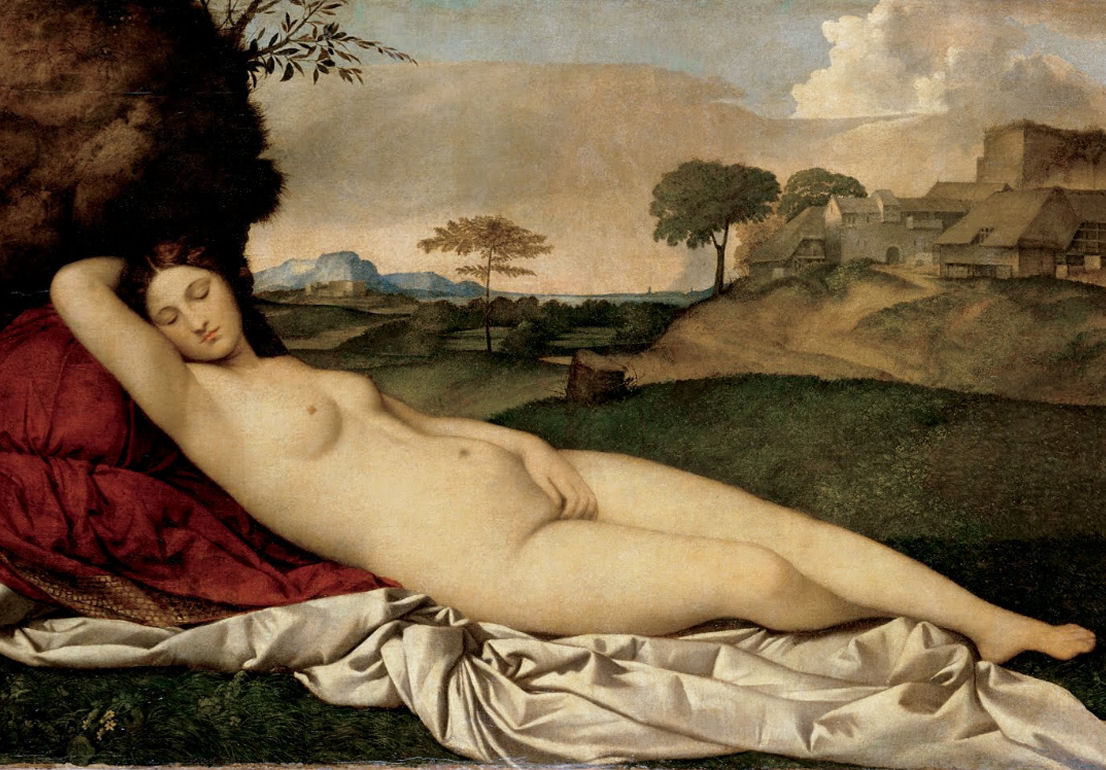
\includegraphics[width=\textwidth]{graphics/Sleeping Venus Giorgione1508-1510.jpg}
%     \caption{Georgione's Dresden Venus 1508-1510}
%     % \label{fig:cave}
%   \end{subfigure}
%   \hfill
%   \begin{subfigure}[b]{0.49\textwidth}
%     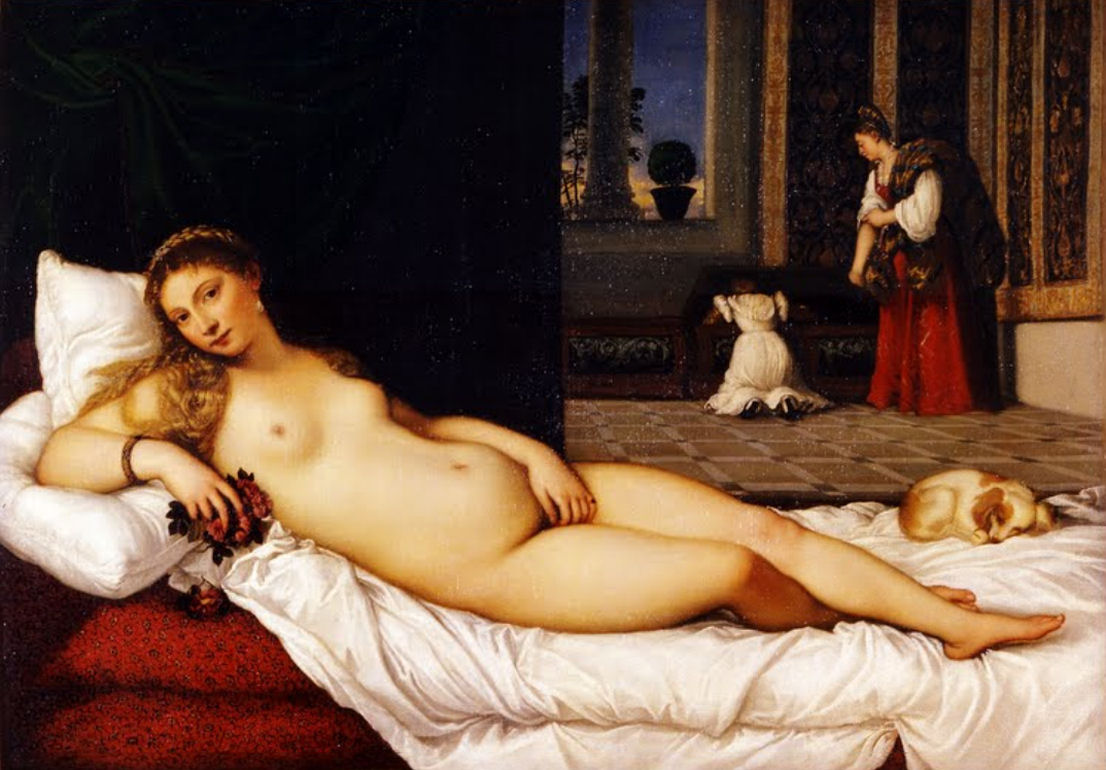
\includegraphics[width=\textwidth]{graphics/Venus of Urbino Titan 1538.jpg}
%     \caption{Titan's Venus of Urbino, 1538}
%     % \label{fig:picasso}
%   \end{subfigure}
%   \caption{Standard image retrieval methods fail to match these paintings as there is substantial difference in appearance.}
%   \label{fig:paintings}
% \end{figure}

% The Dresden Venus by Giorgione (1510)

% Venus of Urbino by Titian (1538)

% If we could build a system that could see the conceptual structure and theme of a text, we could 





% I think Information \textit{Retrieval} will be superseded with Information \textit{Generation} and procedural creativity. Having a machine with \textit{creative} capabilities does not mean they will supersede artists, as computer graphics did not supersede animators. Computers are already tools that artists use, developing computational creativity would just be another tool to use. 

% There are currently many skeptics, who deny that machine can be truly \textit{``creative''}. Inspiration was once thought to be a blessing from the divine.

% \begin{flushleft}
% ``Sing to me Muse...''
% 	\\--- Homer
% \end{flushleft}
% \begin{center}
% ``For the Lord giveth wisdom''
% 	\\--- Proverbs 2:6
% \end{center}
% \begin{flushright}
% ``that Divine accident from the gods, from the mysterious source of the inexplicable''
% 	\\--- Søren Kierkegaard
% \end{flushright}

% In human history, unexplained phenomena are usually credited to divine intervention; eventually, science catches up and gives it a qualifying explanation. Something which cannot be explained feels like magic. The moment you understand an explanation, it transforms into a mere trick. Some prefer not to kill the magic, not look behind the Wizard’s curtain, not explain a joke. But, reverse engineering a construction or a process is the first step in being able to to reproduce it yourself, simulate its external behaviour, or emulate its internal properties.

% However, long before the technological singularity arrives, we will probably get our hands on some super cool search engines.



% \section{Conceptual Semantics}
% Text was replaced with knowledge. The popularity of knowledge graphs as a data structure rose. These graph based, knowledge representations were thought to be a rough approximation of the knowledge structures within our mind. The dream was to build knowledge systems on a massive scale, these highly structured and content-rich ontologies, which we could traverse to find any piece of information, and develop algorithms which could traverse the ontologies for us. A big issue with these systems is that they're expensive to build and maintain, they're essentially infeasible in practice.

% The next ambitious goal for IR research is Conceptual Semantics. A proposed symbol system intended to resemble our thoughts better than language does. If we had an algorithm that could perform \textit{perfect} semantic disambiguation and determine the author's original intent. One could index documents as \textit{conceptual symbols}, not lexical terms. Search queries could also be converted concepts. And performing a search task would involve matching concepts directly. These kinds of systems would not require the effort to manually build or maintain. Such a system could indeed transcend language barriers.

% https://mydailyartdisplay.wordpress.com/2011/02/15/venus-of-urbino-by-titian-and-the-sleeping-dresden-venus-by-giorgione/






% Having a knowledge structure, or ontology, with clearly defined boundaries, and consistent category membership. Is only really ideal building human interfaces. Expecting a person to find a single book from a pile of millions would be infeasible in practice, but shelve those books under filing system, or index, it becomes feasible. Imposing handmade structure onto large volumes of information makes it possible for to navigate, explore, and find what we're looking for. But it appears that handmade, orderly structure is not what makes for  




% language was thought to mirror our cognition
% though it has become increasingly apparent that this is not the case
% language and cognition are related
% but our understanding is when the speaker's intent and the listener's inference agree


%%%%%%%%%%%%%%%%%%%%%%%%%%%%%%%%%%%%%%%%%%%%%%%%%%%%%%%%%%%%%%%%%%%%%%%%%%%%%%%%%%%%
% \section{}


% It should be clear that language is highly ambiguous, but surprisingly our thoughts do not seem to be. At least the thoughts of a healthy, neuro-typical mind are not ambiguous. However, the mind of someone suffering from schizophrenia can have great troubles disambiguating their own thoughts \cite{torrey1985surviving}.

% \begin{center}

% \textit{``Simple words such as `eye' can be substituted for `I' and `to' for `too' or `two'. Homonyms have significant meaning to the schizophrenic, as you can see, or should I say sea. Words like no and know can be used interchangeably. So when I answer a question `no' I may very well be simply asking the question `know?' As in `do you know?' ''}
% \\ --- Surviving Schizophrenia, 6th Edition: A Family Manual
% \end{center}


%%%%%%%%%%%%%%%%%%%%%%%%%%%%%%%%%%%%%%%%%%%%%%%%%%%%%%%%%%%%%%%%%%%%%%%%%%%%%%%%%%%%
        % \chapter{Providing Information}
% \begin{flushright}
%     \textit{``Science, done right, is one of the humanities.''}
%     \\ --- Daniel C. Dennett
% \end{flushright}

On a Starfleet space station orbiting the Vulcan star system, there is a caf{\'e}. This caf{\'e} has an airlock garbage chute, next to the garbage chute is an android, a decommissioned android by somebody who's quite good at

'cos they've switched the robot into a hibernation mode.

Near the staff access to the caf{\'e}, there is a garbage chute.

caAttending service desk is a defunct Starfleet android, on the robot there is a laser engraving, a handmade engraving by someones who's quite good at Word, `cos they flipped the sign into landscape. On the sign in bold letters, it says:

\begin{center}
\textbf{
MALFUNCTIONED: \\
ALL INFORMATION \\
PROVIDED
}
\end{center}

Soong-type android

What is \textit{THAT!?} That sign may well have just said, `FREE MONEY!' What sort of halfwit leaves an apparent Soong-type android by the trash? 

\vspace{5mm}
\begin{center}
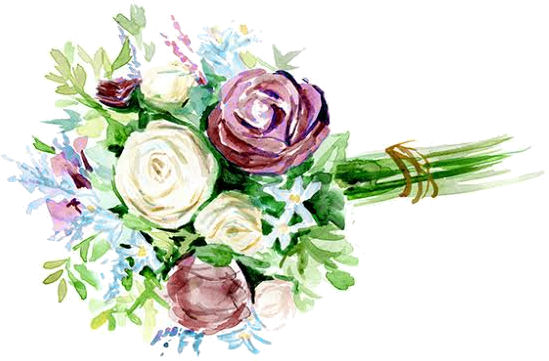
\includegraphics[width=0.45\textwidth]{graphics/flower.jpg}
\end{center}

    
    \cleardoublepage
    \bibliographystyle{plain}
    \bibliography{thesis}
    \appendix

\chapter{Google's Query Expansion Patents}
\label{appendix:googlepatent}
\begin{figure}[h]
    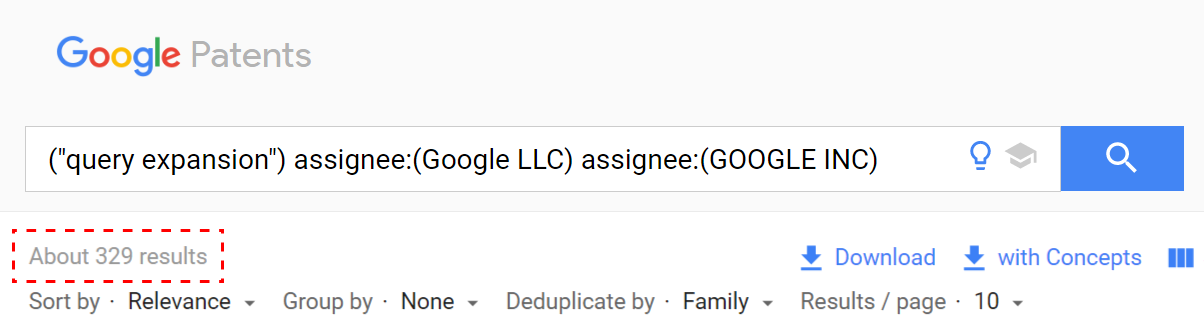
\includegraphics[width=\textwidth]{graphics/google-patents.png}
    \caption{About 329 patents referencing ``query expansion'' owned by Google Inc}
\end{figure}

\begin{table}[h]
\begin{tabular}{ll}
US-9002869-B2    & Machine translation for query expansion                                                                         \\
US-8521761-B2    & Transliteration for query expansion                                                                             \\
US-9146967-B2    & Multi-stage query processing system and method for use with...                               \\
US-9165033-B1    & Efficient query rewriting                                                                                       \\
US-9053115-B1    & Query image search                                                                                              \\
US-8135619-B2    & \textbf{Increasing a number of relevant advertisements using a...}                                            \\
US-9619565-B1    & Generating content snippets using a tokenspace repository                                                       \\
US-9323806-B2    & Clustering query refinements by inferred user intent                                                            \\
US-8600975-B1    & Query phrasification                                                                                            \\
US-8255949-B1    & \textbf{Television program targeting for advertising}                                                                    \\
CN-102349087-B   & Automatically providing content associated with captured information... \\
CN-101796480-B   & Integrating external related phrase information into a phrase-based...       \\
US-8612427-B2    & Information retrieval system for archiving multiple document versions                                           \\
US-9037573-B2    & Phase-based personalization of searches in an information retrieval...                                      \\
\end{tabular}
\end{table}
\begin{table}[]
\begin{tabular}{ll}
US-7617205-B2    & Estimating confidence for query revision models                                                                 \\
US-7870147-B2    & Query revision using known highly-ranked queries                                                                \\
US-7636714-B1    & Determining query term synonyms within query context                                                            \\
US-7565345-B2    & Integration of multiple query revision models                                                                   \\
US-7346615-B2    & Using match confidence to adjust a performance threshold                                                        \\
US-8738553-B1    & Image selection based on image quality                                                                          \\
US-9652483-B1    & Index server architecture using tiered and sharded phrase posting lists                                         \\
US-9183226-B2    & Image classification                                                                                            \\
US-9355169-B1    & Phrase extraction using subphrase scoring                                                                       \\
CN-102226901-B   & Phrase-based searching in an information retrieval system                                                       \\
CN-101133388-B   & Multiple index based information retrieval system                                                               \\
US-7426507-B1    & Automatic taxonomy generation in search results using phrases                                                   \\
US-7580929-B2    & Phrase-based personalization of searches in an information retrieval...                                     \\
US-8996527-B1    & Clustering images                                                                                               \\
US-7702614-B1    & Index updating using segment swapping                                                                           \\
CN-101313300-B   & Local search                                                                                                    \\
US-8825571-B1    & Multiple correlation measures for measuring query similarity                                                    \\
US-2005149499-A1 & Systems and methods for improving search quality                                                                \\
US-9251206-B2    & Generalized edit distance for queries                                                                           \\
US-7925655-B1    & Query scheduling using hierarchical tiers of index servers                                                      \\
US-8452763-B1    & Extracting and scoring class-instance pairs                                                                     \\
US-8832132-B1    & Personalizing search queries based on user membership in social...                             \\
US-9047622-B1    & Delivering content to users based on advertisement interaction type                                             \\
JP-2006048683-A  & Phrase identification method in information retrieval system                                                    \\
JP-2006048685-A  & Indexing method based on phrase in information retrieval system                                                 \\
JP-2006048686-A  & Generation method for document explanation based on phrase                                                      \\
CN-108139849-A   & For the action suggestion of user in selecting content                                                          \\
US-9916396-B2    & Methods and systems for content-based search                                                                    \\
US-9195741-B2    & Triggering music answer boxes relevant to user search queries                                                   \\
US-9507826-B1    & Generating real-time search results                                                                             \\
US-8086594-B1    & Bifurcated document relevance scoring                                                                           \\
KR-20160010652-A & Identifying inadequate search content                                                                           \\
US-10169751-B2   & System and method for point of sale transaction logging                                                         \\
US-2008270364-A1 & Expansion rule evaluation                                                                                       \\
US-8995716-B1    & Image search results by seasonal time period                                                                    \\
\end{tabular}
\end{table}
\begin{table}[]
\begin{tabular}{ll}
CN-107092615-A   & Query suggestion from document                                                                                  \\
US-9767169-B1    & Enhancing search results for improved readability                                                               \\
US-8463783-B1    & Advertisement selection data clustering                                                                         \\
US-8898148-B1    & Targeting to physical environment                                                                               \\
US-8515731-B1    & Synonym verification                                                                                            \\
US-2006230005-A1 & Empirical validation of suggested alternative queries                                                           \\
US-9514223-B1    & Synonym identification based on categorical contexts                                                            \\
US-2015370833-A1 & Visual refinements in image search                                                                              \\
US-8832096-B1    & Query-dependent image similarity                                                                                \\
US-2013018723-A1 & Search-aware conditional bidding on advertisement display                                                       \\
CN-105706135-A   & Supporting voting-based campaigns in search                                                                     \\
US-9218369-B2    & Ranking image search results using hover data                                                                   \\
US-9270712-B2    & Managing moderation of user-contributed edits                                                                   \\
US-8909625-B1    & Image search                                                                                                    \\
US-8538979-B1    & Generating phrase candidates from text string entries                                                           \\
US-9286405-B2    & Index-side synonym generation                                                                                   \\
US-8027938-B1    & Discriminative training in machine learning                                                                     \\
EP-2073131-A1    & Method and apparatus for processing a search query for text content...                                       \\
CN-108463816-A   & Prevent from forbidding the distribution of Web content by using...                    \\
US-9286395-B1    & Modifying query in discourse context                                                                            \\
US-2016307000-A1 & Index-side diacritical canonicalization                                                                         \\
US-10339144-B1   & Search operation adjustment and re-scoring                                                                      \\
US-10460348-B1   & Selection of content items based on internet activity data aggregated...           \\
US-8918381-B1    & Selection criteria diversification                                                                              \\
US-9311362-B1    & Personal knowledge panel interface                                                                              \\
US-2015088859-A1 & Click magnet images                                                                                             \\
US-10122983-B1   & Creating a video for an audio file                                                                              \\
US-6411950-B1    & Dynamic query expansion                                                                                         \\
US-6502091-B1    & Apparatus and method for discovering context groups and document...                \\
US-6385600-B1    & System and method for searching on a computer using an evidence...                                             \\
US-9501571-B1    & Category generalization for search queries                                                                      \\
AU-2011247862-A1 & Integration of multiple query revision models                                                                   \\
US-10691747-B2   & Association of data items and objects                                                                          
\end{tabular}
\end{table}

% \chapter {on Academic Writing}
% Conjecture: Science writing is bad. Readability is reducing over time. Technical language is increasing, with linguistic specificity and precision.

% The Wittgensteinian perspective is that nobody can use language "precisely", it's not only unreasonable, but impossible! Language use is misuse; one man's precision is another man's ambiguity, because what we employ as "language" is closer to an "idiolect" (in both speech and writing). If I offer my family camels, my dad infers a cigarette, but my niece infers the animal. Language as a tool, is a subjective mental construction, which depends on one's own unique experiences. Language is NOT an objective, static, universal tool that dictionaries claim it to be, because we learn the word "camel" through usage in context, not from a dictionary.

% You cannot eliminate the imprecision of language! even if you limit yourself to a "precise" (or technical) vocabulary, or even if you explicitly redefine your own private vocabulary, you'll not escape imprecision. Language is an unstable self supporting structure of sand, and you can't restructure the foundation of sand beneath you to make the walls of sand around you more stable.

% %Removing ambiguities from language using language: is like trying to remove salt from soup using a sieve made of salt.

% My god, even formal languages and programming languages suffer from ambiguity and vagueness (undefined behavior), don't believe that cumbersome monkey mouth flapping is any better at precision. Proving any grammar as unambiguous is an undecidable problem, you'll have better luck proving P=NP.

% It's strictly impossible to be 100\% precise. "Clarity" is often touted as a reasonable goal, but it's equally as subjective and nebulous as the notion of "precision".

% A better goal would be "obviousness", an unequivocal academic proposition should be SO obvious your readers should question why they didn't think of it first. Your readers should be able to guess the conclusions from your premises. Good science should be disappointingly obvious, it's looking behind the wizards curtain and demystifying the magic of reality into a mere trick, a reproducible trick.

% Even something as daunting as quantum mechanics can be explained in an obvious way. Try me.


% \chapter{Academia}
% In the field of Computer Science (and possibly many other fields) there is an understated and often ignored conflict of interest between our collective pursuit of science, and the individual's pursuit of success. Academics are encouraged to write essays that persuade the reader into believing in some contribution to their chosen field. And while it is true that a genuine contribution makes it easier to write a persuasive argument, a persuasive argument doesn't necessitate any inherent value of the scientific content. I have encountered several papers published in reputable journals that appear to exclude crucial information, or apparently vague on specifics, and upon contacting the original authors it becomes clear that certain details were intentionally omitted to make a more persuasive piece of writing. I’m not accusing anyone of lying, but I will bring into question whether honesty and truthfulness is defined only as the absence of lies. If politicians have taught us anything, it’s that you can say nothing but honest statements while simultaneously being intentionally deceptive. Journalists are also known to have written from a deceitful angle because they are immediately rewarded for writing provocatively. Academics are also rewarded for their writing, they're given promotions of status and financial compensation based on their academic output, and so they're encouraged to bullshit their results into a more positive light, and never to publish their failures. If it is a widely accepted truth that we learn from our failures, wouldn't it stand to reason to share these failures? If only to prevent our peers from performing the same research to rediscover the negative results. Because if it's worth knowing, it’s worth writing down.

% The obvious counter argument is that if bad-science is published in a journal, then eventually somebody will discover it when they try to reproduce the results. But this isn't a solution, it's just turning a blind eye. People assume that everything published is unequivocal fact. And people include politicians who make policy based on those facts. And people include journalists who republish those facts in news articles. And people include my mum who can find enough evidence to support her anti-vaccination stance in those news articles, who lives in a society that doesn't have policy disallowing children to go unvaccinated, then she chooses not to vaccinate any of her kids. And people include me who was unvaccinated for the first 23 years of his life. We live in the real world, with real implications.

% This is a far more prevalent issue that anyone outside academia would think, and I’m not claiming there is a mass conspiracy with clandestine meetings to hide the truth from the public. But the public perception is that an academic is a paragon of moral virtue who has the utmost stringent adherence to objective truth studying away in a gleaming tower of ivory elucidating the worlds toughest challenges with clarity. But the reality is that we're all a bunch of people trying our best just like everyone else; and despite our best efforts we're prone to making mistakes just like everyone else; and we're easily persuaded just like everyone else; with unconscious agenda influencing our every action just like every else.

% It’s just an uncomfortable, and embarrassing truth, that is much easier to ignore than to address. From where I'm standing it appears to be a fundamental flaw in how academia works and I can't be the only person to have noticed it. I don't know what an alternative system would look like, I do know it would encourage the publishing of useful failures and hopefully by virtue of that, academics would have a higher proclivity to be more honest. And then hopefully the speed at which we advance knowledge would increase. Just a thought.

% And since this thesis has become a unified collection of both finished and unfinished thoughts which attempt to reach an idea which is far beyond my skill and station to seek... so it would seem a waste to exclude this one.

% You may have noticed that this thesis is missing many formal citations, namely from credible academics, Rumsfeld, Freud, Wittgenstion, Popper, Derrida, Lacan, Grice, Quine, Satre, Kant, Hegel, Plato, God, and a variety of other comedians... this has been intentional partly because I do not care, my time is best spent elsewhere than participating in the charade that academia has deluded itself not to be. But also because none of those authors need the H-index boost. I have adequately cited them by name so any sincere reader will be adequately informed.

% \chapter{Philosophical problems as linguistic puzzles}
% \section{Ethics is a Game}
% Under the Wittgenstein perspective all ethical dilemmas are linguistic puzzles that we can \textit{attempt} to solve by playing within the rules of the language game. This game might be more familiar as a kind of linguistic deconstruction.

% \begin{center}
% So let's play!
% \end{center}

% \subsection{The Starting Position}
% A popular ethical principle proposed by a philosopher during Classical Antiquity: \textit{"Thou shalt not kill"}. Which is an ethical principle that has stood the test of time.

% % and who was clearly inspired by the work of Hammurabi is

% \subsection{Play by play}
% We can infer that this is an elliptical expression which has omitted the word "person" or "living creature", it is unclear which so let us integrate conservatively. 

% Thou shalt not kill any person or living creature. One of the requirements --- necessary and sufficient intentions --- that define "living creature" is that they are "born" from a womb. 

% Thus we can conclude it is unethical to "kill the born".

% Let us consider one of the antonyms of "born", that is everything that is not born, namely the "unborn"

% Is it possible to infer that it is not unethical to "kill the unborn"?

% This is an impossible question to answer... firstly the question is worded ambiguously.

% Specifically the "unborn" is an ambiguous word as there are multiple definitions that could be chosen. Does the word mean those which \textit{will eventually} become born, those which \textit{will never} become born, those which \textit{might} become born, those which is \textit{undecidable} whether it \textit{would} or even \textit{could} be born, or possibly a union of several definitions?

% Let us focus exclusively on the first definition\footnote{The others are left as an exercise for the reader}, the "unborn" being defined as "those which will eventually become born". From this definition we can conclude that "unborn" is synonymous with "fetus".

% Is a "fetus" a "living creature"?

% Well the conventional definition of a fetus does share many intentions with a living creature. Namely they are both material objects made from organic material. A possible hypernym for both is organism. But is all that is made from organic material a "living creature", plants are made from organic material but are not living creatures, because they are not "born" from a uterus (womb).

% when does biological matter become a "person"?

% Is an ovum (egg/gamete) a "person", certainly not, then menstruation would be tantamount to murder, and it's since the ovulation period is around 24 hours.

% The conservative definition of label "person", is assigned at the precise moment of "conception".

% Let us precisely define "conception" as an event, it definitely includes the fusing of gametes, the sperm and ovum unite into a "zygote".

% Is in virtro fertilization (IVF) conception? Can the process of "conception" happen outside the biological "uturus"?

% We can redefine the moment of "conception" arbitrarily as when the zygote is into the endometrium, the inner lining of the uterus.

% which can happen naturally, or interventionally, when the zygote consists of anywhere betwen 8 to hundreds of cells.

% But then we will still have to redefine the terms again if/when it becomes possible to grow a healthy human person outside a uterus.

% This is a never ending chain of definitions, and redefinitions, that ultimately resides in the vague ethical maxim of "thou shalt not kill"

% The rule we "actually" follow in society is "thou shalt not kill, unless you have a good reason to". Which simultaneously captures the nuance of social dynamics, whilst also being fucking useless.

% Unfortunately we cannot refer to God for moral guidance, for he has not once mentioned his stance on gestating embryo outside inside of an artificial uterus. 

% %Now let us climb back down Wittgenstein's ladder.

% Is abortion killing a person?



% Then abortion is unethical. 

% Contraception is not unethical.

% \subsection{Game Over}

% I don't think the game is over yet, can we go further and find a linguistic contradiction?

% I'm not quite certain that my linguistic abilities are without fault so far, I'm an amateur at this language game, so I might start skipping steps in the precise associations between words, but I hope the broad strokes indicate solid linguistic reasoning.

% Let's keep playing the game, and see if we can't get to some contradiction.

% We can redefine the context the fetus lives within

% The wider pragmatics of the situation could be that the pregnant woman is malnourished and will not survive the pregnancy, nor will the gestating fetus survive. 

% Is it ok to kill one "person" so as to prevent two deaths?

% In this situation the answer is yes, it is ok, in both my own opinion, the opinion of every person I've personally asked, and in the law of this country. 

% This is not the trolley problem, because in one outcome EVERYONE dies.

% There are a multitude of scenarios where it is ok to take one life to save another.

% Euthanasia is killing to prevent suffering

% Assisted suicide is ok

% Lethal force in self defence as a last resort against a murderer who has obvious intention to kill yourself, is widely regarded as being the right course of action.

% Even war has been justified by certain people by implicitly playing language games, redefining certain people to be heretics or some other class of subhuman. Historically it was the status quo for a country to be at war with another country, peacetime is the rarity.

% Aside: Willie Apiata is not a NZ hero, he's a cunt with a gun. A cunt who may have behaved bravely under-fire, nonetheless still a cunt. Who chose to join the military; an institution whose primary purpose is to shoot foreigners. This is one particular definition I have personally chosen, and I don't care to explicate my anti-war/anti-military opinion further. But in general I think that Willie Apiaita deserves no respect and I'm glad his marriage fell apart. It's a hypocritical nation that imprisons those who murder people of their nation, and decorate those who murder people of a different nation. He may be \textit{just following orders}, but the orders are malign evil. On a lighter not... Kate Sheppard is a NZ hero, this is the distinction between nationalism and patriotism. When does a thesis become a manifesto? probably when satire becomes propaganda.

% The moral principle we pretend to follow \textit{``Thou shalt not kill"} has many exceptions, and the language game has leads us to include those caveats linguistically into law.

% The actual rule we follow in reality is, \textit{``Don't kill, unless you have a good reason to''}, this is precisely how all human society acts, but it's not precise enough to be useful to any human society. If we were to account for all of the \textit{``good reasons''} we will destroy the illusion of truth. The worst law maker is the one who has deluded themselves into thinking they can write a law both perfect, practical, and without exceptions.

% \section{The Golden Rule}
% All moral principles when expressed in language are subject to the language game, this includes even the most fundamental and universally agreed upon. The golden rule --- also known as the maxim of reciprocity --- has been formulated and reformulated by countless people, across eons, across generations, across nations, across cultures, from The Buddha to my niece.

% realm of idea-space is fractal

% some structures are infinitly recursive, as they reduce into circular arguments

% this game clearly leads to infinite regress, we just have to contrive further scenarios, or develop more precise language to argue more pedantically. So the question becomes, at which point do we reach a good enough consensus?.



% %The following is the maxim of reciprocity from today to ~200BC.

% %\begin{left}
% Collective Wisdom of the 21st Century \\
% \textit{"Treat others as you would like others to treat you"}
% \\
% Islam --- 40 Hadith, 13 \\
% \textit{"love for your brother what you love for yourself"}
% \\
% Christian --- Luke 6:31 \\
% \textit{"and as ye would that men should do to you, do ye also to them likewise"}
% \\
% Judaism --- Talmud, Shabbath 12 \\
% \textit{"What is hateful to you, do not do to your neighbour"}
% \\
% Buddhism --- Udanavarga 5:18 \\
% \textit{"Hurt not others in ways that you yourself would find hurtful"}
% \\
% Hinduism --- Mahabharata 5:15:16 \\
% \textit{"Do naught unto others what you would not have them do unto you"}
% \\
% Ancient Egyptian goddess Ma'at \\
% \textit{``Now this is the command: Do to the doer to make him do."}
% %\end{left}

% Strictly adhering to the golden rule would lead to the abolition of atrocities like chattel slavery, human sacrifice, racism, sexism etc... that is assuming we use a relatively recent definition of ``others" to include every nationality, race, culture, gender class etc... Which clearly wasn't the case historically. In the above quotes Islam used the word ``brother". Christianity used the word ``men". Judaism used the word ``neighbour". All of which can lead to subjective definitions that are potentially problematic. 

% The Buddhist, Hindu and Ancient Egyptian forms of the Golden Rule appear to have relatively less amount of sublimated bigotry implicit in the language, likely because their languages lacked any linguistic sophistication to articulate those ideas.  double edged sword.

% The most fundamental way to express an abstract idea in natural languages is through the use of metaphor, if the language doesn't have the word that denotes 'blue' you would make a metaphor against something which is known to be blue, 'you eyes are the sky'. Since abstractions are more generalisable than concrete ideas religious text tended towards the flowery language of the metaphorical (possibly also for aesthetic reasons). God is too abstract a concept to explain in concrete language, which is why God has an seemingly unending list of metaphorical titles: the Alpha and Omega, the Fountain of Life, the Father, the Sheppard, the Bread, the Lamb, the Rock, the way and the truth and the life... this has leads to the rise of Igtheism which states it's impossible to believe in something which is by definition unable to be defined. This has also lead to the rise of Pantheism which proposes that God must be everything, the entirety of the material universe, and the infinity of the immaterial.

% %but why risk the possibility of misunderstandings, why not be precise in language? Unnecessarily flowery language should be relegated to the aesthetics.

% But even with the broad definition of ``others'' in the Golden Rule we can still play the language game and arrive at behaviour that is conventionally considered unethical by many, and behaviour that is definitely paradoxical, that is to say undecidably ethical.

% \begin {center}
% \textit{The masochist says to the sadist, ``beat me."
% \\To which the merciless sadist replies, ``NO!"}
% \end{center}

% ``A masochist derives pleasure from being hurt; so denying the masochist his pleasure through-pain hurts him just as much as actual physical pain hurts the non masochist. If a person wants to be hurt and enjoys suffering, then there is no reason not to indulge him in his want.'' --- Anton Szandor LaVey

% The traditional linguistic formulation of the Golden Rule has developed many caveats and exceptions since it was first composed because society has become more nuanced, as has the language we use to express it with. The most recent paradox I asked myself was whether the tolerant should tolerate the intolerant?\footnote{Karl Popper also discovered this linguistic paradox, which appears in his 1945 book ``The Open Society and Its Enemies''... two idiots, same thought.} Immanual Kant attempted to close the loopholes that existed in his time when he redefined the Golden Rule into the \textit{Categorical Imperative}:

% \begin{center}
% \textit{``Act only according to that maxim whereby you can, at the same time, will that it should become a universal law"} \\--- Immanuel Kant
% \end{center}

% and many other people have further critiqued Kant's linguistic formulation of the maxim of reciprocity (Kant's Axe), and for good reason, it's flawed by inherent subjectivity's, just like every other ethical principle expressed with language. Further, all sentences constructed with language (written or spoken) are subject to the language game.


 
 
 
% \chapter{Humour}

% \section{Philosophical Investigations into Humour}

% The opinions of prominent philosophers, including myself.

% The Ethics, Aesthetics and Psychology of Humour.

% Read more of:
% --- Cicero
% --- Bergson
% --- Kierkegaard
% --- Bakhtin
% --- Francis Hutcheson

% %Most quotes have been edited for brevity.
% %Aphorisms on the philosophy of humour.

% \section{Eastern Opinions}
% It's difficult to extract the opinions of eastern thinkers on humour, as they didn't directly state them. But rather much of their wisdom was delivered in joke form.

% \section{Laughter is the Emotion of Scorn}

% Early opinions on humour were unkind.

% Laughter is hostile, we object to hostility.

% \textit{``Laughter is malign evil ... to take delight in another's self ignorance''}\\ -- Plato, Philebus 347 BC

% When an American Idol contestant is ignorant of their inability to sing, we laugh; then we laugh harder when Simon Cowell begins a statement with \textit{``not to be rude, but...''}.
% %suggests their mother had an abortion. 
% %One of American Idol's worst contributions to society is promulgating the incorrect notion that singing is an innate talent and not a learnable skill.

% The professional comedy playwrights Aristophanes and Euripides wrote jokes about Ugliness, Stupidity, Drunkenness, Obesity, Baldness, Farts, Sexual-Innuendo and Phalli, and if their work is an accurate representation of the common humour in Ancient Greece then Plato's parochial opinion is understandable.

% Aristotle was less critical, with an early formulation of the Benign-Violation theory.

% \textit{``blunder or ugliness that does not cause pain or disaster''} - Aristotle 

% \section{The Superiority Theory}

% 1,300 years later humour opinions had evolved into Superiority Theory
% which is essentially the same opinion

% I assume common humour was much the same too

% \textit{``people with very obvious defects such as those who are lame, blind of an eye, hunched-backed, or who have received some public insult, are specially given to mockery''} \\ --- Descartes, The Passions of the Soul 1649

% \textit{``some laughter is caused by deformed thing in another''} \\ --- Hobbes, Leviathan 1668

% \textit{``laughter at the defects of others, is a sign of cowardice''} \\ --- Hobbes, Leviathan 1668

% Mockery, Teasing, Ridicule and Roasting are tools of the Bully and the Satirist.

% \textit{``Laughter expresses a sudden glory arising from some conception of some eminency in ourselves, by comparison with the infirmity of others, or with our''} --- Hobbes

% Bergson wrote a whole book on Laughter.

% His humour theories are still still based on scorn and humiliation



% \subsection{Schadenfreude}
% Pleasure in the misfortune of others.

% ``joy mingled with hatred... perceiving some small evil in a person whom we consider to be deserving of it'' --- Descartes, The Passions of the Soul 1649

% ``To feel envy is human, to feel schadenfreude is diabolic'' --- Schopenhauer, On Human Nature 1890

% ``To laugh means: to be maliciousness but with a good conscience.'' --- Nietzsche, Gay Science, 1882 

% ``To see others suffer does one good'' --- Nietzsche, Ecce Homo 1908

% ``It's always funny until someone gets hurt. Then it's just hilarious'' --- Bill Hicks

% ``Tragedy is if I cut my finger, Comedy is if you walk into an open sewer and die'' - Mel Brooks






% \section{Psychology}

% \textit{``Laughter is an emotion that overrides rational self control''} -- Plato

% Another criticism by Plato; the deliberate thinking man avoids instinctive behaviour... I wonder to want lengths he would go to avoid natural bodily functions.

% Nietzsche's laughter response delay.

% A momentary transition whilst fear resolves into it's opposite. From high-alert lethal-threat defense-mechanism of the animal towards the formality, security, tradition of the expected behaviour in the dependable man. 

% Human, All Too Human, 1878

% I understand the Koestlerian Theory of Incongruity as caused by emotive-speed being slower than logic-speed. Subversion awareness juxtaposed with delayed anxiety.




% I understand the Aristotelian Surprise Theory and it's self evidently accurate. A joke isn't funny the second time, the predictablility lacks surprise.

% I understand the Aristotleian Benign Violation Theory ``A blunder or ugliness which does not cause pain or disaster is laughable''


% I understand the Kantian humour theory as extravagantly limited. "The sudden rise of expectation into nothing" explains only quintessential anti-joke. A bore of a conversationalist.

% I understand the Gricean Cooperative Principle of Conversation, and it's an accurate explanation as to why being an uncooperative belligerent in conversation is the soul of wit. ``wit is educated insolence'' -- Aristotle


% Lord Shaftesbury, An Essay on the Freedom of Wit and Humor 1709
% I understand the Freudian Relief Theory as the stinking pile of misleading reflexive-analogy horse-shit that it is. 
% A functional model if you're a Russell Brand who can raise libidinal levels with a wink.



% Nietzsche’s oppositional transition between extremities. Treating death, suffering or purposeless as not trivial but delightful.



% Being rude in expectation of politeness takes to stabilise into 100% stable.

% Benign-violation 

% Superiority 
% Laugh at others (misfortune, ignorance, schadenfreude, self deprecation) 
% Incongruity 



% Creativity and humor are two “hardwired” characteristics of humanbeings (Darwin, 1872/1965; Maslow, 1943






% \section{Aggressive Theory of Humour}
% These are my thoughts. All are original, but only some are unique, as they are shared with other humorists alive today. 

% There are three primary modes of aggressive humour, and they're subjectively perceived as:

% Disagreeable humour.
% Neutral humour.
% Agreeable humour.

% These modes directly relate to the joke target.
% Insult humour and satire.
% Observational humour
% Neutrality of innocent wordplay.

% Explicit Target - usually a person, possibly the self. 
% Self enhancing, vs Self Deprecating.
% Enhancing and Deprecating.

% Implicit Target - a simple concept, or everyday situation.

% Direct aggressive.
% Indirect aggressive.

% Offensive aggressive.
% Defensive aggressive.

% Defensive Aggressive is the best.

\end{document}

% \bibliographystyle{otago}